\RequirePackage{setspace}
\documentclass[oneside,12pt,a4paper]{Classes/CUEDthesisPSnPDF}
\usepackage{longtable}
\usepackage{lscape}
\usepackage{amssymb}
\usepackage{amsmath}
\usepackage{amsthm}
\usepackage{geometry}
\usepackage{titlesec}
\usepackage{amsfonts}
\usepackage{graphicx}
\setcounter{MaxMatrixCols}{30}
\usepackage{tabu}
\usepackage{setspace}
\usepackage{threeparttable}
\usepackage{multirow}
\usepackage[capposition=top]{floatrow}
\usepackage{color, colortbl}
\usepackage{lscape}
\usepackage{ragged2e}
\geometry{left=4.0cm,right=2cm}
\usepackage{pdfpages}
\usepackage{chngcntr} 
\counterwithout{footnote}{chapter}
\renewcommand{\baselinestretch}{1}
\usepackage{charter}
%******************************************************
\usepackage{float}
\usepackage{footmisc}
\usepackage{array}
\usepackage{booktabs}
\usepackage{tabularx} 
\usepackage{rotating}
\usepackage{sectsty}
\usepackage{floatrow}
\usepackage{caption}
\usepackage[round]{natbib}
\usepackage{appendix}
\usepackage{chngcntr}
\usepackage{etoolbox}
\usepackage{lipsum}

\newcommand{\E}{\mathbb{E}}
\newcommand{\var}{\mbox{Var}}
\newcommand{\cov}{\mbox{Cov}}
\setlength{\arraycolsep}{0.02in}

\AtBeginEnvironment{subappendices}{
\section*{Appendix}}
%******************************************************

\title{Essays on the Economics of Heterogeneity}

\ifpdf
  \author{\href{}{NILS-HOLGER GUDAT}}
  \collegeordept{\href{}{School of Economics and Finance}}
  \university{\href{}{Queen Mary, University of London}}
  \author{NILS-HOLGER GUDAT}
  \collegeordept{School of Economics and Finance}
  \university{Queen Mary, University of London}
\fi
\degree{Doctor of Philosophy (Ph.D.) in Economics}

% turn of those nasty overfull and underfull hboxes
\hbadness=10000
\hfuzz=50pt
\doublespacing
\pretolerance=10000
\tolerance=2000
\emergencystretch=10pt

\usepackage{hyperref} 

\begin{document}
\pagenumbering{gobble} %do not put page number on front page
\begin{titlepage}
\thispagestyle{plain}
\hfill\\
\hfill\\
\vspace{1cm}

\begin{center}
\textbf{\LARGE Essays on the Economics of Heterogeneity}

\vspace{3cm}

\textbf{\normalsize A thesis submitted in partial fulfillment of the requirements \\
\medskip
of the degree of Doctor of Philosophy (Ph.D.) in Economics \\
}

\vspace{3cm}

\textbf{\large Nils-Holger Gudat}

\medskip



\vspace{40pt}

School of Economics and Finance\medskip

Queen Mary, University of London\medskip

October 2015\medskip
\vspace{40pt}


\end{center}
\end{titlepage}
\endinput


\begin{titlepage}
\thispagestyle{plain}
\hfill\\
\hfill\\
\vspace{1cm}

\begin{center}
\textbf{\LARGE Essays on the Economics of Heterogeneity}

\vspace{3cm}

\textbf{\normalsize A thesis submitted in partial fulfillment of the requirements \\
\medskip
of the degree of Doctor of Philosophy (Ph.D.) in Economics \\
}

\vspace{3cm}

\textbf{\large Nils-Holger Gudat}

\medskip



\vspace{40pt}

School of Economics and Finance\medskip

Queen Mary, University of London\medskip

October 2015\medskip
\vspace{40pt}


\end{center}
\end{titlepage}
\endinput


\pagenumbering{arabic} %must put after because of gobble to avoid numbering title page

\begin{dedication}      %this creates the heading for the acknowlegments

\thispagestyle{plain}

\textit{To Nadien, who had to lift my spirits more than once over the last four years; \\ 
				my mother, as I couldn't have made it here without her love and support; \\
				and Emil, whose laugh carried me through the final stages of this project.}

\end{dedication}

\begin{onehalfspacing}

\begin{declaration}      %this creates the heading for the acknowlegments

\thispagestyle{plain}

\textbf{I wish to declare}

I, Nils-Holger Gudat, confirm that the research included within this thesis is my own work or that where it has been carried out in collaboration with, or supported by others, that this is duly acknowledged below and my contribution indicated. Previously published material is also acknowledged below.

I attest that I have exercised reasonable care to ensure that the work is original, and does not to the best of my knowledge break any UK law, infringe any third party's copyright or other Intellectual Property Right, or contain any confidential material.

I accept that the College has the right to use plagiarism detection software to check the electronic version of the thesis.

I confirm that this thesis has not been previously submitted for the award of a degree by this or any other university.

The copyright of this thesis rests with the author and no quotation from it or information derived from it may be published without the prior written consent of the author.\\

\textbf{Details of collaboration and publications:}\\
Parts of Chapter \ref{ch:trade} were undertaken as joint work with Ryan Weldzius (University of California, Los Angeles).\\

\textbf{Signature:} Nils-Holger Gudat \\
\textbf{Date:} \today


\end{declaration}

\end{onehalfspacing}

% Thesis Acknowledgements ------------------------------------------------

\begin{onehalfspacing}
%\begin{acknowledgementslong} %uncommenting this line, gives a different acknowledgements heading
\begin{acknowledgements}      %this creates the heading for the acknowlegments

\thispagestyle{plain}

I would like to thank my supervisors, Xavier Mateos-Planas and Winfried Koenieger, for their guidance, patience and support throughout my Ph.D. studies.  \\\\
I further acknowledge the School of Economics and Finance at Queen Mary, University of London, for generous funding. 

\end{acknowledgements}
\end{onehalfspacing}

\begin{abstractslong}
\thispagestyle{plain}

The analysis of the effects of heterogeneity on aggregate economic outcomes has 
seen a resurgence in the recent macroeconomic literature. The exponential increase
 in computer power over the last decades has allowed researchers to solve ever 
more complex theoretical models with meaningful heterogeneity along various 
dimensions, while at the same time bringing ever more granular micro-level data 
to the table when testing the model predictions. \\
This thesis explores two varieties of this recent vintage of models of heterogeneity.
The first part of the thesis investigates the implications for wealth distributions
of combining the standard life-cycle incomplete markets model of household 
consumption with income processes featuring heterogeneity in individual-specific
growth rates, which households can learn about over the course of their working life.
To this extent, first the recent literature on partial insurance and models
of wealth inequality is reviewed. Then, income processes with profile heterogeneity
 are estimated from PSID and BHPS data. Finally, the estimated income processes
are used in a quantitative model of household consumption and saving, which is 
calibrated to empirical wealth distributions obtained from the SCF and the BHPS.
Comparative statics exercises are performed to identify the drivers in the models
success (or failure) to match the empirical profile of wealth holdings.
The second part of the thesis looks at heterogeneity on the production side of 
the economy and its implications for international trade. Following an existing 
approach in the literature, we develop testable implications of the Melitz and 
Ottaviano (2008) model of trade, in which firms differ in their 
productivity and have to make production and exporting decisions in the face of 
costs to trade. Our approach allows us to test the effects of NAFTA on productivity 
in 64 manufacturing sectors in North America and thereby complement and extend
 the existing literature on the effects of trade liberalisations.
\end{abstractslong}

%set the number of sectioning levels that get number and appear in the contents
\setcounter{secnumdepth}{2} %number sections and subsections
\setcounter{tocdepth}{1}

\begin{spacing}{1.3}
  \tableofcontents
\end{spacing}

\begin{spacing}{1.5}
	\listoftables
	\listoffigures
\end{spacing}

\chapter{Introduction} %preface is not numbered
\markboth{\MakeUppercase{\thechapter. INTRODUCTION}}{INTRODUCTION}
\section{Motivation}
Distributional questions are increasingly making a comeback in economics. 


\section{Outline}
This thesis is structured as follows. Chapter 2 gives an overview of the research on theoretical models of the household wealth distribution in the last two decades. It will highlight the key empirical challenges by presenting stylized facts on the cross sectional wealth distribution in a number of countries and their evolution over time. Then, an overview of existing modeling approaches is presented,  

Chapter 3 builds on the discussion in Chapter 2 by constructing a model of learning about idiosyncratic income processes and using it to simulate wealth distributions. As a first step, income processes with profile heterogeneity are estimated for different sub-periods of PSID data from 1968 to 1999 and from BHPS data in order to assess the stability of the cross-sectional variance of income growth rates across time and labor markets. The estimates are then used as inputs in a structural model of household saving first employed by \citet{Guvenen2007}, with the addition of both structural breaks in the cross-sectional variance of growth rates and habits in consumption. The models predictions for the evolution of the US consumer wealth distribution are then benchmarked against data from the Survey of Consumer Finances. 

Chapter 4 gives a brief introduction into trade models based on firm-level heterogeneity, before developing an estimable model in the spirit of \citet{Chen2009}. The model is then tested on a data set of prices, productivity, and markups for nine manufacturing industries in the Canada, Mexico and the United States over the period of 1994 to 2010. In an extension of the approach of \citet{Chen2009}, we also conduct a sub-sample analysis in which we split the same into fixed and free entry industries, based on a measure of firm turnover developed on the basis of prior research. 

Chapter 5 concludes the thesis and discusses potential avenues for future research. \ref{sec:conclusion}

\chapter{Models of the wealth distribution} %\label{chap:atsm} 
\markboth{\MakeUppercase{\thechapter. WEALTH DISTRIBUTION MODELS}}{WEALTH DISTRIBUTION MODELS} 
\section{Introduction}

The distribution of wealth and income has recently made a comeback to the
centre of economic discourse in advanced economies. The ongoing rise of
income inequality, observed since the early 1980s especially in Anglo-Saxon
countries, has received renewed attention in the public sphere since the
financial started taking its toll on living standards across the world. At
the same time, the best-selling book by \citet{Piketty2014} led to a surge
in interest in the role of capital in the economy, and, by extension, the
distribution of wealth, both in the academic literature and the popular
press. \\
While the broader public has only recently picked up on the issues arising
around income and wealth distributions, they have sat squarely in the centre
of many sub-fields of economics for a long time. The income distribution has
long been of interest to labour economists trying to understand the forces
shaping the evolution of earnings in the labour market, while at least the
accumulation of aggregate wealth plays a central role in macroeconomic
models of economic growth. This chapter, as well as chapter three, 
focuses on the intermediate step that takes us from an
income to a wealth distribution - economic models of household saving.
When attempting to build a model of the wealth distribution, the first
step of course is to get an understanding of the object we want to model.
To this end, this chapter starts by presenting stylised facts of the wealth
distributions in advanced countries and discusses some of the limitations
of the data available. It then builds a simple life-cycle model of consumption
and savings to guide the following discussion and fix notation. Using this
basic model, different savings motives and their importance in the context
of aggregate wealth accumulation are discussed. Following this, the role of
income uncertainty and market structure is examined in more detail.


\section{Stylised facts}
The most notable and consistent fact that emerges when looking at wealth
distributions across all countries and different time periods is that wealth
is highly unevenly distributed, much more so than income. This can be readily
seen when comparing Gini indices and top shares of income and wealth, as in
Table \ref{tab:gini_topshares} or looking at histograms and cdfs of wealth and
income distributions as in Figure \ref{hist_cdfs}. It is important to note
that in producing these aggregate numbers and figures, one necessarily has
to make decisions on how exactly to construct measures of income and wealth,
which will have to be kept in mind when comparing model predictions with
empirical numbers. When constructing an income measure, the obvious starting
point are labour earnings, and for many economic applications simply
observing an individual's wages will be enough. When thinking about questions
of consumption smoothing though, we are ultimately interested in accounting
for all claims on consumption goods available to an individual or household
in a given period, and while for most people the largest part of these claims
stem from labour earnings, we will also want to account for the effect of
government programs (by constructing a post-tax, post-transfer income measure),
income from accumulated assets, and potentially even informal insurance
arrangements such as inter-vivos transfers between family and friends.
In constructing wealth measures, we again have to think closely about the
question we are trying to answer when constructing them. If the goal is to
account for all productive capital in the economy that can be used in
production, a measure of total net wealth aggregating all forms of asset and
debt classes, and including some durable consumption goods such as cars. When
thinking about the role of wealth in helping the household to smooth out
income fluctuations, it might be more appropriate to exclude very illiquid
assets such as housing, and look more closely at the role of debt for households
which might be at their borrowing constraint and are thus vulnerable to
reductions in their borrowing limit, even though their net wealth (including
illiquid assets) is positive. Finally, important questions are raised by
the existence of various government and private pension schemes, which have
to be factored in when constructing measures of a household's lifetime
resources, but whose exact value might be uncertain (for the case of defined
contribution plans) and not well understood by households themselves.


\begin{table}%
\begin{tabular}{lcr}

\end{tabular}
\caption{Measures of wealth concentration in different data sets.}
\label{tab:gini_topshares}
\end{table}

\begin{figure}
\includegraphics[width=\columnwidth]{}
\caption{Histograms and cdfs of household net wealth in different data sets.}
\label{hist_cdfs}
\end{figure}

\section{A workhorse model}
The basic model underlying the discussion of savings behaviour and wealth 
accumulation in this chapter is the life-cycle model of household behaviour 
dating back to \citet{ModiglianiBrumberg1954} \footnote{A more detailed 
treatment of the general class of models can be found both in 
\citet{BrowningCrossley2001} and in \citet{AttanasioWeber2010}, although both 
papers have their focus on household consumption behaviour rather than wealth 
accumulation.}. The model can be written as a single household solving the 
problem

\begin{align}
\max_{\{c_{t+j}\}_{j=0}^{T-t}} \sum_{j=0}^{\infty} \delta^{t+j} \mathbb{E}_t \big[ u(c_{t+j}, z_{t+j}) \big] \label{maxprob}
\intertext{subject to} 
a_{t+1} = (1+r)(a_t + y_t - c_t) \label{bc}
\end{align}
where $T$ is the last period of the planning horizon, $\delta$ is the subjective
discount factor, $u()$ is the instantaneous felicity function -- usually assumed
to be of the CRRA form, $\frac{c^{1-\sigma}}{1-\sigma}$, where $\sigma$ is the 
coefficient of relative risk aversion --, $c$ is 
consumption, $a$ are financial assets, which allow the household to transfer 
resources across time, $r$ is a one-period interest rate, and $y$ is income. 
$z$ is used as a stand-in variable denoting the fact that households might, 
in general, care about other things that are not captured by the concept of 
current consumption; examples would be habits or durable consumption (which 
break the time-separability of the utility function), leisure time, particular 
classes of assets (such as housing) or bequests left to future generations.  
While in general, $T \rightarrow \infty$ is a possibility, and infinite horizon 
versions -- first advocated by \citet{Friedman1957} -- of the life-cycle model 
are widely used in macroeconomic applications, the finite horizon model will be 
more useful for the following discussion and forms the centrepiece of this 
thesis for a number of reasons which will become clear as we progress.

\section{Saving motives}
When trying to understand wealth distributions through the lens of the model
outlined above, the key question is: why do households save? The basic model,
in which consumers only care about the time path of instantaneous utility 
derived from consumption, suggests that households will save if and only if
it leads to preferential allocation of consumption over time -- they engage 
in consumption smoothing. As \citet{BrowningCrossley2001} point out, consumption
smoothing can happen at different frequencies, depending on the exact set-up 
of the model. In \citet{ModiglianiBrumberg1954} the main reason saving was the
existence of a retirement period, which necessitates consumption smoothing over
the life cycle -- wealth accumulation during working life to pay for consumption
in retirement. The implication of this simple model is that wealth accumulation
on the household level solely depends on the length of the retirement period, 
while in aggregate wealth accumulation crucially hinges on the growth rate
of the economy. The crucial assumption that allows Modigliani and Brumberg to
focus on consumption smoothing over the life cycle was that of constant income.


\section{Income uncertainty and market structure}
With the assumption of a non-constant income stream, it becomes important to 
think about the opportunities households have to insure themselves against
these fluctuations. 

\section{The role of housing}
\citet{CampbellHercovitz2005}
\citet{Yang2009}
\citet{Iacoviello2008}

\section{Closed and open economies}
On the endogeneity of interest rates

\section{Wealth Distribution Papers}
In the last years, many authors have used the increasing possibilities offered
by the increase in computing power to derive an additional implication from the
broad class of incomplete market models outlined above: a simulated wealth 
distribution. While there are many practical difficulties in creating model 
outputs that can reasonably compared to the data collected in surveys (some of
which have been alluded to in the above discussion on the definition of wealth),
in principle the simulated wealth distribution derived from life-cycle models
can be used to calibrate deep parameters of the model, provide an additional
test for how well the model is able to capture household savings behaviour, 
and shed light on which mechanisms are crucial in driving the evolution of 
aggregate savings at different parts of the distribution. \\
An early attempt to use the wealth distribution to estimate the parameters of
a life-cycle model of household savings can be found in \citet{Cagetti2003},
who uses a simple model similar to the one outlined in equations \ref{maxprob}
and \ref{bc}. Important additions in his version of the model are a bequest 
motive -- which, ceteris paribus, will increase the wealth holdings of elderly
households -- and a simplified pension system, which guarantees each household
a pension depending on their education level, and thereby lowers wealth 
accumulation during working life. The idea behind the estimation strategy is 
simple: given a stochastic process for household income, the parameters $\beta$,
$\sigma$ and $\alpha$ pin down a solution to the household's savings problem 
which allows one to simulate a theoretical wealth distribution from optimal 
household behaviour. Therefore, it is possible to use the simulated method of
moments to construct an estimator that chooses the triplet $(\delta,\sigma, 
\alpha)$ which minimises the distance between empirical moments of the wealth
distribution and its simulated counterparts. Given the high skewness of wealth
data, Cagetti opts for median wealth by 5-year age group as the moment to match.
As has become clear in the previous discussion, a crucial element driving 
household choices in the model is the income risk they face, making the choice
for the stochastic process representing this risk and its calibration a crucial
step in modelling wealth distributions. Cagetti opts for a process consisting
of a trend growth component common to all households, an age-education component
estimated for CEX data, and an MA(1) process representing the stochastic nature
of income. With his calibration, Cagetti finds low degrees of persistence, with
pronounced heterogeneity across education groups, and high degrees of risk 
aversion, implying a significant contribution of precautionary savings to 
aggregate wealth. \\
A very similar exercise is performed by \citet{HintermaierKoeniger2011}, who 
construct a minimum distance estimator based on the shape of the cross-sectional
distribution of wealth at different stages of the life cycle. That is, rather
than simply targeting the 50th percentile of wealth holdings  as 
\citet{Cagetti2003}, here all percentiles of the wealth distribution from 10 
to 90 are considered. The reason for excluding the upper ten percentiles of the
distribution are the well-known problems that a simple life-cycle model has in 
matching the extreme levels of wealth concentration observed at the upper end 
of the distribution, which might be driven by other motives than the buffer-
stock and retirement savings motives included in the model. Increasing the 
number of moments to match leads to estimates of the discount factor which are 
an order of magnitude more precise than in \citet{Cagetti2003}. The estimate for
the discount factor, at $\hat{\delta}=0.985$, is at the upper bound of the
estimates in \citet{Cagetti2003}, while the estimated risk aversion parameter
$\hat{\sigma}=1.08$ is only a third to one sixth as large as Cagetti's estimate,
depending on the subgroup under consideration.  


\citet{HintermaierKoeniger2011}
\citet{CastanedaRiosRull2003}
\citet{DPMRR2003}
\citet{Floden2008}
\citet{BenhabibBisinZhu2011}
\citet{DeNardiYang2015}

\section{Conclusion}
This chapter provides an overview of stylised facts about the wealth 
distributions in a number of advanced economies and presents various approaches 
to build economic models which can account for these stylised facts.
It became clear that while saving for retirement is the main driver of wealth
accumulation for large parts of the population, other factors need to be taken
into consideration to explain the tails of the distribution and the behaviour of
young households. Crucial aspects of an economic model of the wealth 
distribution are the risks households are facing -- both on the income and the 
expenditure side -- and the financial markets available to them to insure 
themselves against those risks and earn returns on their savings. Finally, the 
far right tail of the wealth distribution seems to be driven by factors beyond 
this and it is not clear whether variation in subjective discount factors, 
entrepreneurial activity, or other factors are best suited to model wealth 
accumulation at the top.
 

\chapter{The effects of profile heterogeneity on estimates of income risk} \markboth{\MakeUppercase{\thechapter. PROFILE HETEROGENEITY AND INCOME RISK}}{PROFILE HETEROGENEITY AND INCOME RISK}
\section{Introduction}
As has become clear from the discussion in the previous chapter, a crucial 
ingredient to any model of household savings is an estimate of the risk that
households are facing in the form of their income process. While traditionally
researchers have relied on a parsimonious AR(1) specification with a transitory
and a persistent shock component, which can be represented as a Markov chain 
and thus helps to ease the computational burden. Recent research has cast doubt 
on the ability of this specification to accurately capture the risk faced by 
households in the labour market though, and advances in computational 
capabilities have allowed to solve models with larger state spaces, so that 
there is a renewed interest in estimating richer statistical processes for 
household income. \vspace{1cm}
\\
\textbf{Insert discussion of recent papers based on social security data:
\citet{GKOS2015}, \citet{DHPRV2013}}

\section{A statistical model}
To inform the simulations in the following chapter, this thesis will rely on an
estimated heterogeneous income profiles (HIP) income process in the spirit of
\citet{Guvenen2009}. The process to be estimated is of the form

\begin{align}
y_{h,t}^i &= g(\theta_t, \pmb{X}_{h,t}^i) + \alpha^i + \beta^i h + z_{h,t}^i + \phi \varepsilon_{h,t}^i \label{incproc} \\ 
z_{h,t} &= \rho z_{h-1,t-1} + \pi_t \eta_{h,t}^i \label{persshock}
\end{align}

where $y_{h,t}^i$ are the log earnings of individual $i$, who has $h$ years of
labour market experience in period $t$. The function $g()$ is assumed to be 
a cubic polynomial in experience, while the individual specific parameters 
$\alpha^i$ and $\beta^i$ -- modelled as random variables with mean zero and 
variance $\sigma^2_{\alpha}$ and $\sigma^2_{\beta}$, respectively --
 capture the cross-sectional profile heterogeneity. 
$z_{h,t}^i$ is an AR(1) process with persistence $\rho$ and innovation variance
$\eta_{h,t}^i$, which captures persistent shocks to income, while
$\varepsilon_{h,t}^i$ is a purely transitory shock. Both $\eta^i$ and 
$\varepsilon^i$ are mean-zero i.i.d random variables with variances 
$\sigma^2_{\eta}$ and $\sigma^2_{\varepsilon}$, respectively. As discussed 
above, the variances of both permanent and transitory shocks have seen large
swings over the past decades, to capture this we are allowing for time-variation
in the innovation variance (denoted $\pi_t$ for the innovation to the persistent
shock component and $\varphi_t$ for the transitory counterpart). \\
To estimate the parameters of the model, an equally weighted minimum distance 
estimator is used to minimise the distance between the empirically observed 
variance-covariance structure of residual earnings (defined as $\tilde{y} \equiv 
y_{h,t}^i - g(\theta_t, \pmb{X}_{h,t}^i)$ and the variance-covariance 
structure implied by the model. In the present context, this strategy has first 
been employed by \citet{Baker98}, who estimates a very similar model to the one
 described above, although the approach has been used before for estimating 
other models in labour economics, e.g. \citet{AbowdCard89}. Our model implies 
theoretical variances and covariances given by:
\begin{align}
\var(\tilde{y}_{h,t}^i) = \underbrace{\sigma^2_{\alpha} + 2 \sigma_{\alpha \beta} h + \sigma^2_{\beta}}_{\text{contribution of profile heterogeneity}} + \var(z^i_{h,t}) + \phi_t^2 \sigma^2_{\varepsilon} \\
\cov(\tilde{y}_{h,t}^i, \tilde{y}_{h+n,t+n}^i) = \underbrace{\sigma^2_{\alpha} + 2 \sigma_{\alpha \beta} (h+n) + \sigma^2_{\beta}} + \var(z^i_{h,t}) + \phi_t^2 \sigma^2_{\varepsilon}
\end{align}
The empirical variance-covariance matrix underlying the estimation will be 
obtained by first calculating the covariance of residuals for each age-group
in a given year, and then averaging over all age groups present in a given year.
The theoretical counterpart is obtained by simply calculating the corresponding
variances and covariances from the formulas above, and forming weighted averages
over $h$ with weights corresponding to the relative frequency of age-groups in 
the empirical data. 

\section{Data}
The data is taken from all available waves of the PSID, that is years 1968 to
2013 inclusive\footnote{Note that the PSID income variable refers to income in 
the previous year, so when we talk about data from, e.g., year 1968, it is 
implied that we are referring to income in 1967.}. For our baseline estimation,
to ease comparisons, we stick to the sample selection criteria used in 
\citet{Guvenen2009}, namely:
\begin{itemize}
	\item Household heads between the ages of 20 and 64 inclusive
    \item Hourly labour earnings between \$2 and \$400 in 1993 prices
    \item Hours worked between 520 and 5110
\end{itemize}
For inclusion in our sample, an individual has to fulfil all of the above
conditions for at least 20, not necessarily consecutive, years. These sample
selection criteria leave us with 1685 individuals in our final sample
\footnote{To create the longitudinal data set from the PSID cross-sections, we
use the excellent \textit{PSIDtools} package \citep{Kohler2015}}. The main 
variable of interest in the analysis is labour income, for which we use the 
series of variables starting with \texttt{V74} in 1968\footnote{A complete of 
all variables used is available on  
\href{https://github.com/nilshg/psidJulia/blob/master/create_panel.do}{my GitHub
page}.}. Hourly earnings are taken from the variable starting with \texttt{V337}
in 1968, while hours worked are taken from the variable starting with 
\texttt{V47}. 
 

\section{Results}
\begin{table}%
\begin{tabular}{l|cccccc}
                    &$\rho$ & $\sigma^2_{\eta}$&$\sigma^2_{\varepsilon}$&$\sigma^2_{\alpha}$&$\sigma^2_{\beta}$&$\sigma_{\alpha \beta}$\\
\hline
\hline \\
Guvenen (2009), RIP & 0.988 &  0.015           &   0.061                &       --          &        --        &        --             \\
Guvenen Matlab, RIP & 0.935 &  0.010           &   0.023                &       --          &        --        &        --             \\
Short sample, RIP   & 0.951 &  0.011           &   0.043                &       --          &        --        &        --             \\
Full sample, RIP    & 0.920 &  0.014           &   0.067                &       --          &        --        &        --             \\
\hline
Guvenen (2009), HIP & 0.821 &  0.029           &   0.047                &   0.022           &     0.00038      &     --0.23            \\
Guvenen Matlab, HIP & 0.853 &  0.013           &   0.030                &   0.030           &     0.00031      &     --0.30            \\
Short sample, HIP   & 0.855 &  0.017           &   0.018                &   0.022           &     0.00030      &     --0.32            \\ 
Full sample, HIP    & 0.839 &  0.017           &   0.064                &   0.047           &     0.00026      &     --0.32            \\ 
\hline
\end{tabular}
\caption{Results for the PSID sample 1968-1996; Guvenen (2009) refers to published results, Guvenen Matlab to results obtained by running
the code available on the journal website, short sample to my own estimation with the 1968-1996 data, full sample to the 1968-2013 data.}
\label{hip_rip_results}
\end{table}




\chapter{The implications of learning about income processes in the face of structural breaks for the household wealth distribution} \markboth{\MakeUppercase{\thechapter. LEARNING AND THE WEALTH DISTRIBUTION}}{LEARNING AND THE WEALTH DISTRIBUTION}
\section{Introduction}
The preceding two chapters have pointed out the importance of developing quantitative
economic models of household saving and the important interconnections between
savings, insurance, and income risk. This chapter builds on the discussion of 
the previous chapter by calibrating a model of household saving featuring a
heterogeneous income process to empirical data on the wealth distribution and
assessing the models fit under different parametrisations of the income process.
The main finding is that including profile heterogeneity significantly worsens
the models ability to fit the data moments, a finding which is robust across
all income processes estimated in the previous chapter. We then conduct comparative
statics exercises to explore what drives this result. These exercises show that
it is precisely the main difference that separates HIP from RIP processes --
the lower estimated persistence and variance of transitory shocks -- which 
keeps the model from matching the shape of the empirical wealth distribution. 
While lifetime inequality in an income distribution simulated from an HIP process
with modest amounts of profile heterogeneity is just as high as that found in an
income distribution simulated from a persistent AR(1) process with high innovation
variance, the different mechanism generating this inequality crucially alters
household savings behaviour. 
\vspace{0.5cm}   \\
The model employed  in this chapter is a standard incomplete markets life-cycle 
model of household  
consumption and savings as described in chapter \ref{ch:wealthmodels}, with the
addition of a learning mechanism for household income, as first used by 
\citet{Guvenen2007}. While this model has recently been used to study household's
portfolio choices (\citealt{ChangHongKarabarbounis2015}) and the joint evolution 
of income and consumption inequality in a rich dynamic model featuring informal
insurance mechanisms (\citealt{GuvenenSmith2014}), the implications of heterogeneous
income processes and learning for the aggregate wealth distribution have so far
not been examined to the best of our knowledge.
Although a very early working paper version of \citet{Guvenen2007} briefly comments
on the wealth distribution that obtains in a model of profile heterogeneity and
learning\footnote{At the time of writing, the working paper can be accessed at
\url{http://www.usc.edu/schools/business/FBE/seminars/papers/M_5-18-04_GUVENEN-Labrisk04.pdf}.},
noting that overall wealth accumulation is significantly higher than in a model
without profile uncertainty, to the best of our knowledge no further investigations
into the ability of life-cycle models with profile heterogeneity to match the 
wealth distribution have been undertaken. Given the recent evidence discussed 
in chapter \ref{ch:income} pointing towards profile heterogeneity as an important
feature of real life income processes, it is important to understand what including
these income processes in life-cycle models -- arguably making them reflect
better the actual risk facing households in reality -- means for the wealth 
distribution predicted by the model. While chapter \ref{ch:wealthmodels} showed
that there are many promising extensions to the standard model making it conform
better to the empirical wealth distribution, virtually all papers discussed there
rely on a simple AR(1) process with persistent and transitory shocks for the 
modelling of income risk, a process that, if the HIP specification estimated 
in chapter \ref{ch:income} is correct, significantly overstates both the magnitude
and the persistence of permanent shocks to household income. Therefore, this 
chapter examines theoretical wealth distributions coming out of models relying
on the HIP process for household income, under the assumption that households 
are imperfectly informed about the parameters of their individual income 
process, but able to learn them over the course of their working life. Using the
parameter estimates from chapter \ref{ch:income}, it explores the implications
of changes over time and across household income measures for the predicted
wealth distribution. Following \citet{HintermaierKoeniger2011}, it then uses 
a minimum distance estimator to calibrate discount factor and risk aversion in
order to minimise the difference between wealth holdings at different percentiles
of the wealth distribution in the model and the data. Then, comparative statics
exercises are performed to isolate the role of the different parameters of the
HIP process in determining the shape of the income distribution. Finally, the 
sensitivity of the model to changes in agents' initial beliefs and the role
of systematic mistakes in beliefs is investigated.


\section{The Model}\label{sec:model}

Consumers maximize
\begin{align}
E_t &\left[ \sum_{i=0}^{T-t} \beta^{i} \frac{c_{t+i}^{1-\sigma}}{1-\sigma} \right] \label{eq:maxprob} \\
\intertext{s.t. } &a_{t+1} = (1+r)a_t + y_t - c_t \label{eq:bc} \\
				  &y_{t}^i = \begin{cases} (\theta^0, X_t^i) + f(\theta^i, X_t^i) + z_t^i + \epsilon_t^i \label{eq:incproc} &  \text{ for } t<R \\
                                           y^R & \text{ for } t>= R
                             \end{cases} \\
  				  &a_{t+1} \geq \underline{a} \label{eq:borrcons} 
\end{align}
where $c_t$ is consumption in period $t$, $a_t$ are asset holdings subject to 
a borrowing constraint  $\underline{a}$, and $y_t^i$ is individual 
income, which follows the heterogeneous income specification in logs discussed
in chapter \ref{ch:income}: 
\begin{equation*}
y_{t}^i = g(\theta^0, X_t^i) + f(\theta^i, X_t^i) + z_t^i + \varepsilon_t^i 
\end{equation*}
Here, $g(\theta^0, X_t^i)$ captures age effects and individual specific 
characteristics such as experience and education\footnote{In keeping with chapter three, 
$\theta^0$ will be modelled as a cubic polynomial in experience, with the parameters
obtained from a pooled regression on the data underlying the estimates in that 
chapter.}, $z_t^i$ is an autoregressive process of order one equivalent to 
the one used in chapter 3, $\varepsilon$ is a transitory shock following a standard normal 
distribution and $f(\cdot)$ is an individual specific function that plays the decisive
role in introducing heterogeneity and learning in the model. Here, $f(\cdot)$ 
is defined as:
\begin{align*}
f(\theta^i, X_t^i) &= \alpha^i + \beta^i t \\
\theta^i &\sim N \left[ \begin{pmatrix} 0 \\ 0 \end{pmatrix}, \begin{pmatrix} \sigma_{\alpha}^2 & \sigma_{\alpha \beta} \\ \sigma_{\alpha \beta} & \sigma_{\beta}^2 \end{pmatrix} \right]
\end{align*}
The parameters $\alpha$ and $\beta$ are randomly distributed over the population 
and govern the evolution of lifetime income over time. Furthermore, they are 
unknown to individuals upon entering the labour market, meaning that in order to
 calculate an expected lifetime income to base consumption choices on, consumers 
in the model have to form beliefs over the values of their individual parameters. 
Here again we follow Guvenen in assuming that these beliefs are formed optimally
in a Bayesian fashion, which means solving a Kalman filtering problem. 
Denoting by $S^i_{t+1}$ the vector of parameters $\alpha^i$, $\beta^i$ and 
$z^i_{t+1}$ and by $F$ the coefficient vector in the state space representation,
the evolution is governed by the law of motion:
\begin{align}
\hat{S}^i_{t|t} &= \hat{S}^i_{t|t-1} + P_{t|t-1} H_t [H_t' P_{t|t-1} H_t + R]^{-1}(y_t^i - H_t' \hat{S}^i_{t|t-1}) \label{eq:KFS} \\
\hat{S}^i_{t+1|t} &= F \hat{S}^i_{t|t} \label{eq:TES}
\end{align}
where we denote by $\hat{S}^i_{t|t}$ the optimal estimate of the individual specific
parameters of the income process in period $t$ after having observed the realisation
of $y_t^i$, and by $\hat{S}^i_{t+1|t}$ the optimal forecast based on those beliefs,
assuming that the transition matrix $F$ is known to the household. $P_{t|t}$ is 
the variance-covariance matrix of $\hat{S}^i_{t|t}$ and $R$  is the variance of 
the transitory shock. A similar expression can be derived for the evolution of 
$P_{t+1|t}$:
\begin{align}
P_{t|t} &= P_{t|t-1} - P_{t|t-1} H_t [ H_t' P_{t|t-1} H_t + R]^{-1} H_t' P_{t|t-1} \label{eq:KFP} \\
P_{t+1|t} &= F P_{t|t} F' + Q \label{eq:TEP}
\end{align}
With $Q$ denoting the covariance matrix of the innovation in the state space 
representation of $\hat{S}_{t+1|t}^i$ (which is basically the innovation in the 
AR(1) component of earnings). 
Given this formulation for the evolution of beliefs, we can write the recursive 
version of our maximization problem as:
\begin{equation} \label{eq:bellman}
V_t(x_t,\hat{S}^i_{t|t}) = \max_{\{c_t^i\}} \left\{ u(c_t) + \mathbb{E}_t \left[ V_{t+1}(x_{t+1},\hat{S}^i_{t+1|t+1}|\hat{S}^i_{t|t}) \right] \right\}
\end{equation}
which again has to be solved subject to the constraints, \ref{eq:bc}, \ref{eq:borrcons} 
and \ref{eq:KFS}-\ref{eq:TEP}. Note that given this formulation of the problem, 
all state variables appearing in the continuation value function on the right-
hand side of the Bellman equation are functions of the realisation of income 
next period, so that the expectation in \ref{eq:bellman} has to be taken only 
with respect to $\hat{y}^i_{t+1}$. The distribution of next period's expectation
of income is known exactly, conditional on current beliefs:
$$ 
\hat{y}^i_{t+1} \sim \mathcal{N}(\hat{\alpha}_{t|t} + (t+1)\hat{\beta}^i_{t|t} + \rho \hat{z}_{t|t}, \sigma^2_{\alpha} + t^2 \sigma^2_{\beta} + 2t\sigma_{\alpha \beta} + \sigma^2_{\eta} + \sigma^2_{\varepsilon}
$$
An important issue when trying to match empirical wealth distributions is the 
specification of the pension system. The household problem during retirement is 
straightforward to solve in the absence of uncertainty; it is given by
\begin{align}\label{eq:retirement}
V^R_t(a_t,\bar{y}) &= \max_{c_t, a_{t+1}} u(c_t) + \delta V^R_{t+1}(a_{t+1},y^R)
\intertext{s.t.}   &a_{t+1} = (1+r)a_t + \bar{y} - c_t \\
				   &y^R =  M(\bar{y}, \bar{Y})\\
  				   &a_{t+1} \geq \underline{a}
\end{align}
where $M$ is a benefit function that emulates the US Social Security system and 
is specified following much of the literature on life-cycle models (cp. 
\citet{STY2004}, \citet{HintermaierKoeniger2011}, \citet{GuvenenSmith2014}, 
amongst others) as a function depending on average lifetime income  of an 
individual, $\bar{y}$, relative to the economy-wide average income $\bar{Y}$:
$$
y^P = \begin{cases} 0.9\bar{y} & \text{if} \bar{y} < 0.3\bar{Y}  \\
    0.27 + 0.32(\bar{y} - 0.3) & \text{if} \bar{y} \leq 2.0\bar{Y} \\
    0.814 + 0.15(\bar{y}- 2.0) & \text{if} \bar{y} \leq 4.1\bar{Y} \\
           1.129 \bar{Y}       & \text{if} \bar{y} > 4.1 \bar{Y}
      \end{cases}
$$
Note that this system attenuates the inequality in lifetime income created by 
the stochastic process for income by providing higher replacement rates for 
poor households than for rich households. To avoid adding another state variable
to the model, we replace the true value of $\bar{y}$ by an estimate derived
from running the cross-sectional regression 
$$
\bar{y}_i = k_0 + k_1 y_T^i
$$
where $i$ denotes one agent in our simulation. The coefficients $(k_0, k_1)$ are
then used to predict an agent's average lifetime income for the purposes of 
determining his pension entitlement based on realised income in the final period
of working life. With an R-squared of 0.9, this regression gives a reasonable 
estimate of the true lifetime income of an agent.    

\subsection{Computational Algorithm}
To solve the model, we adopt a strategy similar to that in \citet{GuvenenSmith2014}.
After drawing an income distribution and simulating agent's learning given a set
of initial beliefs, we construct a three-point grid for $\hat{\alpha}$, a 
fifteen-point grid for $\hat{\beta}$ and a seven-point grid for $\hat{z}$, all
linearly spaced ranging from the lowest to the highest belief coming out of the
simulation of agent's learning process. For wealth, we choose 40 grid points, 
exponentially spaced with a higher concentration of points at low levels of wealth.
The choice of grid size is motivated by an iterative procedure, in which the model
is repeatedly solved using finer grids in each step until an additional grid point
in a given dimension makes an insignificant contribution to the resulting wealth
distribution coming out of the simulation. 
The income processes underlying the simulations are taken directly from the estimations
in \ref{ch:income}, with the $g()$ function chosen such that the average life-cycle
profile for income tracks that in the PSID or BHPS data. 
The household's pension problem can be solved analytically -- as there is no 
uncertainty and the utility function allows for an analytical expression of the 
Euler equation, a closed-form solution for consumption as a function of the 
pension level and retirement wealth can be obtained --, while the household's 
working life problem is solved recursively on all grid points in the four-
dimensional state space. To evaluate the continuation value function on the right-
hand side of the Bellman equation, we employ quadrilinear interpolation combined
with Gauss-Hermite quadrature on ten nodes for the numerical integration
\footnote{In particular, the linear interpolation was performed using the 
\texttt{ApproXD.jl} package \citep{Oswald2014}, while the Gauss-Hermite nodes
were derived using the \texttt{FastGaussQuadrature.jl} package \citep{Townsend2015}.}. In the
simulation step, we initialise household wealth holdings by drawing from the empirical 
wealth distribution for 23 to 25 year old households from the Survey of Consumer
Finances, data that is available in \cite{HintermaierKoeniger2011}. We check 
the sensitivity of model results to this choice by comparing them to the 
alternative of zero wealth holdings at age 20 for all households and confirm both
that there is no qualitative difference in model results, and that the quantitative
differences are negligible. All codes used in this chapter can be found in my 
GitHub repository \href{https://github.com/nilshg/LearningModels}{LearningModels}.


\section{Quantitative Results}\label{sec:qr}
To take the model to the data, we follow the strategy in \citet{HintermaierKoeniger2011}
and calibrate the model using a minimum 
distance estimator that minimizes the difference between wealth holdings at percentiles 
10 to 90 of the net wealth distribution for different ages. The values for the 
SCF can be readily obtained from the code of \citet{HintermaierKoeniger2011}, 
while we use the UK Wealth and Asset survey to derive similar statistics for the 
UK for fitting the model when the income process is derived from BHPS data.
The target moments in the data are the wealth holdings at percentiles 10 to 90
for prime age households (ages 26 to 55), as well as for young (ages 26 to 35), 
middle aged (ages 36 to 45) and old (46 to 55) households\footnote{When using 
WAS data, the age categories are all shifted back by one year (that is, young 
households are aged 25 to 34), as this is the categorisation used in the survey.},
which gives us a total of 324 moments to match. Stacking all of these moments
into a vector $\mu$, and denoting the vector of percentile wealth holdings
for households simulated from the model by $\theta$, the minimum distance estimator is 
$$
\min_{\delta, \sigma} \theta' I \theta
$$
\citet{HintermaierKoeniger2011} derive a normality result for the estimates obtained
from this estimator, which allows us to compute standard errors as the main 
diagonal of the inverse of the squared Jacobian, $trace((J'J)^(-1)$, where
$$
J = \left[ \frac{\partial \theta}{\partial \delta} \frac{\partial \theta}{\partial \sigma} \right]
$$
As our baseline estimate, we fit the HIP process estimated from the full sample 
of PSID households from 1968 to 2013 in chapter \ref{ch:income}. From the minimum 
distance estimation, we obtain a discount factor of $\delta=0.973$ and a risk 
aversion parameter $\sigma=1.90$ as the best fit, although the value of the objective
function at the minimum is still very high. The reason for this can be seen
graphically in figure \ref{fig:baseline} and figure \ref{fig:baseline_agedetail}:
the model entirely misses the shape of the empirical wealth distribution, predicting
too little wealth at the low end of the distribution, too high 
wealth accumulation for households between the 20th and 70th percentile, and
too small wealth holdings again for households at the highest percentiles
\footnote{Note that in all plots, we only display wealth holdings in model and 
data between the first and 90th percentile.}. Breaking the result down by age 
groups, we see that young households are much poorer in the model than they are
in the data, while older cohorts display much higher savings. 

\begin{figure}
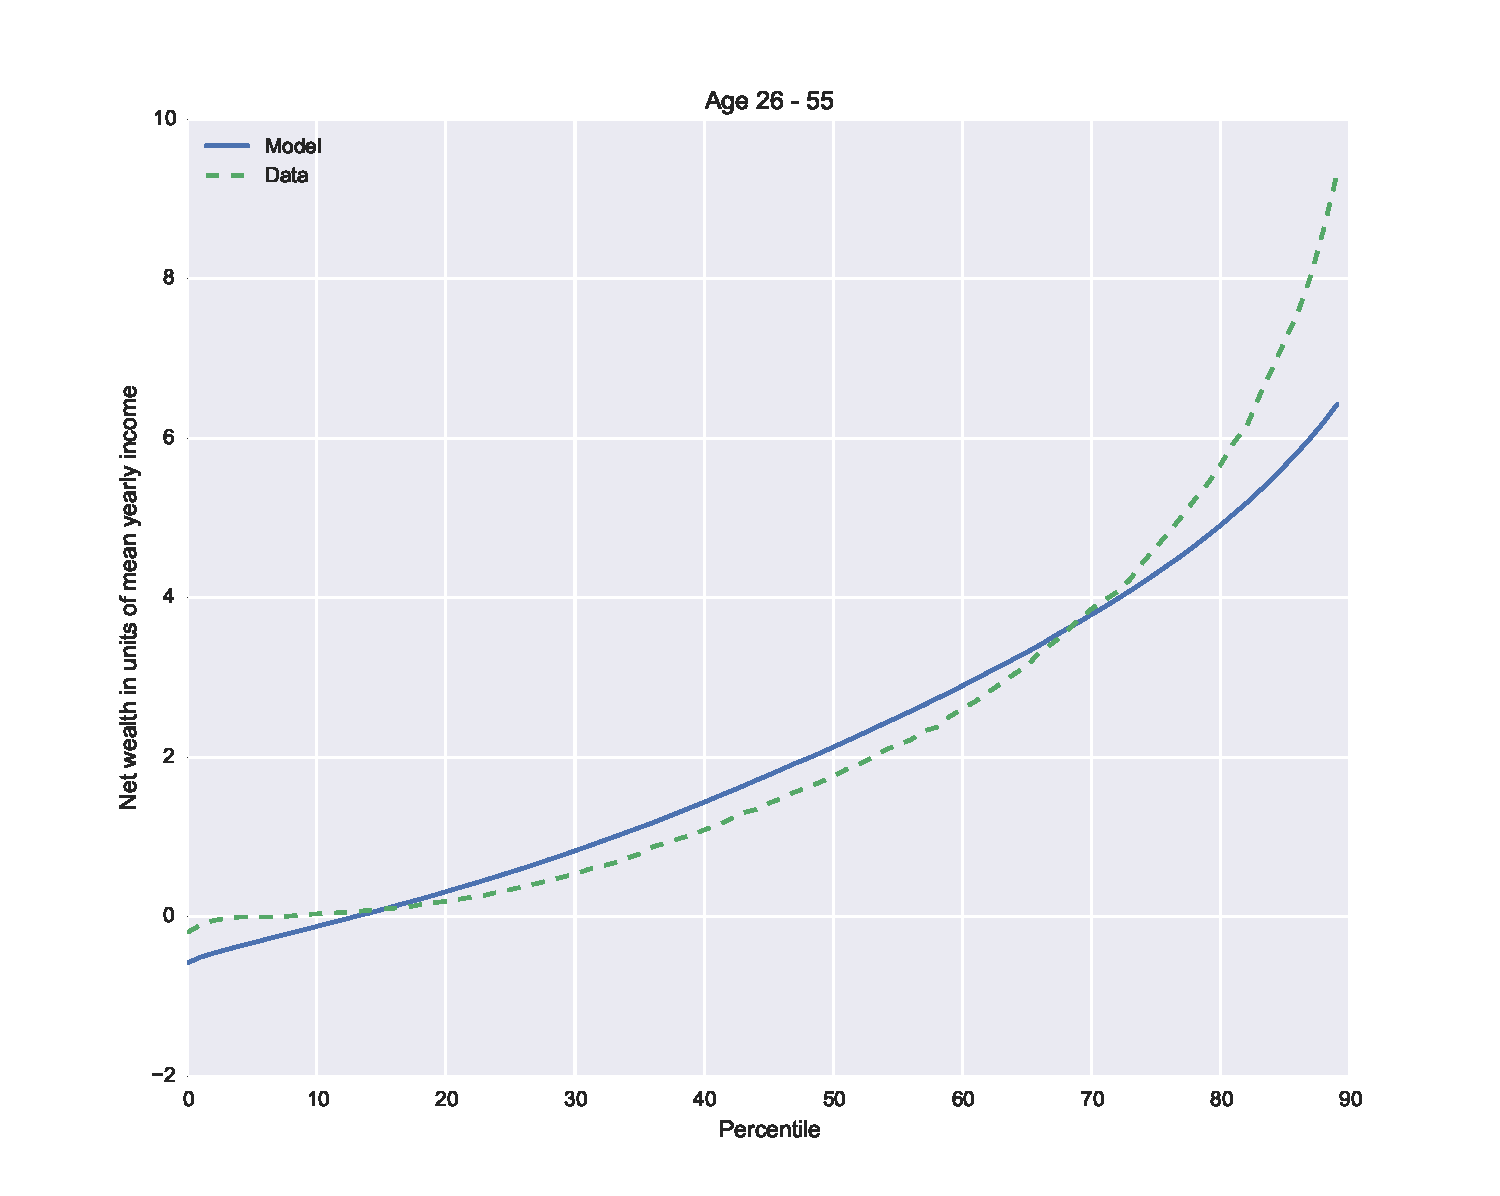
\includegraphics[width=\columnwidth]{baseline}
\caption{Baseline model (PSID HIP income process), calibrated fit}
\label{fig:baseline}
\end{figure}

\begin{figure}
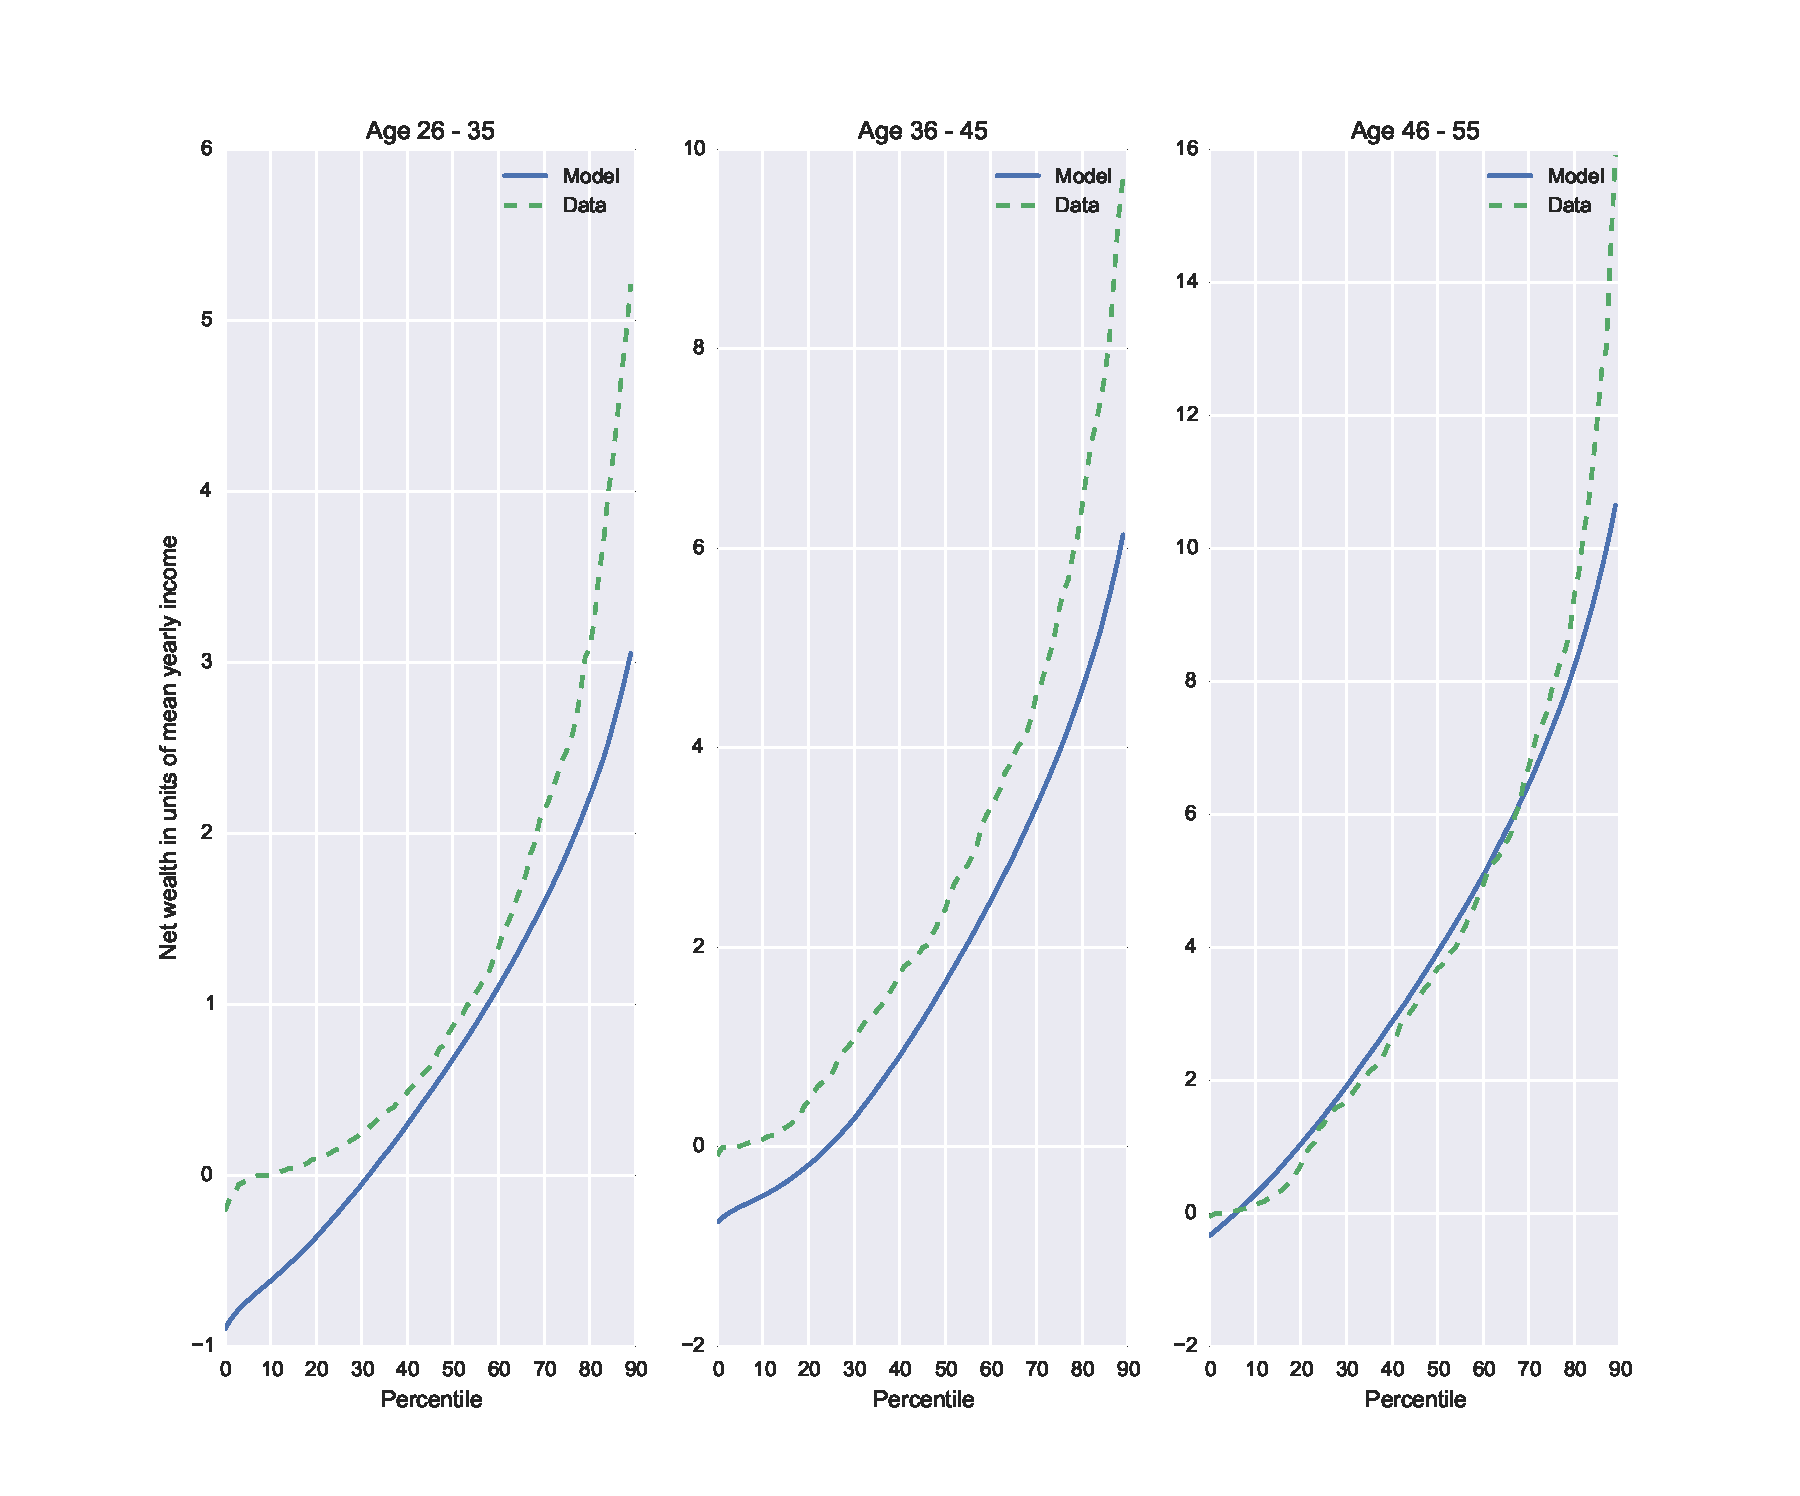
\includegraphics[width=\columnwidth]{baseline_agedetail}
\caption{Baseline model (PSID HIP income process), calibrated fit by age group}
\label{fig:baseline_agedetail}
\end{figure}


From these results
it is obvious that the shape of the wealth distribution predicted by the model
is so fundamentally wrong that none of the processes estimated in chapter 
\ref{ch:income} will stand a chance of matching the empirical wealth distribution.
In the interest of brevity, we therefore skip a graphical presentation of the model
fit for the processes estimated from BHPS data to the empirical wealth distribution
in the WAS, and only report the results of the minimum distance estimation in 
table \ref{tab:calibration_results}. It can be seen that all estimates of the 
discount factor are significantly lower than those obtained by \citet{HintermaierKoeniger2011},
an artefact of the fact that overall wealth accumulation in the life-cycle model
featuring an HIP income process is much higher than in a comparable model 
relying on a simple AR(1) income specification, as reported in the earlier 
working paper version of \citet{Guvenen2007}. In the first row, we also report 
the results for fitting a model using the HIP parameters estimated from the PSID
data, but excluding the deterministic life cycle profile of earnings, 
$g_t(\theta_0, X_t^i)$, which is the exact income process used in \citet{Guvenen2007}.
The results show that the estimated discount factor is almost exactly that 
used in Guvenen's paper, at 0.961, and importantly significantly lower than 
all other discount factors, estimated including the respective life-cycle profiles
of earnings extracted from the different data sets. Intuitively, this result
stems from the fact that without the deterministic income profile, the mean 
of households' expected earnings distributions is much closer to zero, creating
a larger precautionary savings motive. The minimum distance estimator then tries
to counterbalance this by choosing a lower discount factor, increasing aggregate
savings by making households more patient. This suggests that the increase in 
aggregate savings coming from an HIP based model as reported in the earliest 
working paper version of \citet{Guvenen2007} is somewhat overstated when 
the life-cycle profile of earnings is disregarded\footnote{Although it has to 
be noted here that, at least for our measures of gross labour incomes, the processes
we estimate might understate the true "disaster risk" in income, given that the 
sample selection process excluded households with zero earnings. \citet{GKOS2015}
make some effort to alleviating this problem by introducing a mixture of AR(1)
components into an HIP process, with one of the AR(1) processes capturing the 
very low likelihood of extremely large shocks to household income.}. 

\begin{table}
\begin{tabular}{l|c|c}

       Income Process            & $\delta$ & $\sigma$ \\
\hline                          
PSID 1968-2013 (no lifecycle)    &  0.961 & 1.41    \\
                  & \footnotesize{(0.0008)} & \footnotesize{(0.006)} \\ 
PSID 1968-2013 (with lifecycle)  &  0.973 & 1.90    \\
                  & \footnotesize{(0.0008)} & \footnotesize{(0.006)} \\
BHPS gross labour income         &  0.967 & 0.621    \\
                  & \footnotesize{(0.00027)} & \footnotesize{(0.041)} \\
BHPS net labour income           &  0.965 & 0.5    \\
                  & \footnotesize{(0.00046)} & \footnotesize{(0.036)} \\
BHPS net household income        &  0.975 & 1.28     \\
                  & \footnotesize{(0.0069)} & \footnotesize{(0.166)} \\

\end{tabular}
\caption{Calibrating the model for different income risk profiles}
\label{tab:calibration_results}
\end{table} 


\section{Comparative Statics}\label{sec:comp_stats}
Given the largely disappointing results of the calibration and simulation exercises,
we now turn to some comparative statics exercises to elicit what features of the 
model are crucial to get closer to the shape of the observed wealth distribution.
To do so, we pick a reasonable baseline calibration from the set of available 
parameters estimated for different income processes in chapter \ref{ch:income}, 
and then vary each of the 8 parameters governing the model solution by solving 
the model in turn for its highest and lowest realization. The parameter values
used are summarized in table \ref{tab:comp_stat_parameters}. It is noted that these
simulations are meant to be illustrative only, and explore the sensitivity of the
model results with respect to a given parameter. They can not be directly mapped
to any real world counterpart, as fixing one of the parameters of the income 
process at a given value would require re-estimation of the remaining parameters
as described in \ref{ch:income} to ensure that the new process represents as 
closely as possible the true underlying income risk households are facing.

\begin{table}
\begin{tabular}{l|cccccccc}
                  & $\delta$ & $\sigma$ & $\rho$ & $\sigma^2_{\eta}$ & $\sigma^2_{\varepsilon}$ & $\sigma^2_{\alpha}$ & $\sigma^2_{\beta}$ & $cov(\alpha,\beta)$ \\
                \hline
Lowest realization  &  0.94  &  1.05  & 0.72   &    0.01           &    0.02                  &     0.01            &      0.00068       &    -1.     \\
Baseline            &  0.96  &  2.0   & 0.85   &    0.03           &    0.05                  &     0.05            &      0.00038       &    -0.3    \\
Highest realizatoin &  0.98  &  3.0   & 0.92   &    0.05           &    0.13                  &     0.10            &      0.00001       &     0.     \\
\end{tabular}
\caption{Parameters for comparative statics}
\label{tab:comp_stat_parameters}
\end{table}

Changing the variance of the cross-sectional distribution of intercepts does not
influence the results in any meaningful ways, as could have been anticipated 
from the fact that $\alpha$ in effect parallel shifts the entire life-cycle
profile of households up or down, which, given that almost all households are 
far enough away from the borrowing constraint at all times, and in the absence
of any different savings behaviour of rich households in the model (as e.g. found
in the data by \citealt{DSK2004}), means that savings behaviour is not affected
by this change. Similarly, changing the variance of the transitory shock does 
not alter the results significantly, save for an overall increase in wealth holdings
for the highest value of $\sigma^2_{\varepsilon}$\footnote{Graphical results can be found
in the Appendix}.
The two parameters that have a markedly larger influence on the \textit{shape}
of the predicted percentile distribution, and hence help the model get closer
to the data moments, are the persistence of the AR(1) component and the variance
of its innovations. Figures \ref{fig:comp_stat_rho} and \ref{fig:comp_stat_rho_agedetail} 
show the effects of varying the persistence of the AR(1) component of the income 
process for prime age households and households by age group, respectively. When
increasing $\rho$ to 0.92, the predicted wealth distribution becomes notably more
curved, while the effect of lowering $\rho$ from 0.85 to 0.72 is significantly 
smaller. This is not very surprising, as the implications of lowering $\rho$
for the half-life of a persistent shock become less severe the lower the starting
value of $\rho$ -- as figure \ref{fig:effect_rho} demonstrates, the half life
of a persistent shock under the baseline $\rho=0.85$ is about four years, while 
for $\rho=0.72$ it is two years and for $\rho=0.92$ it is eight years. The model
with a high value of the persistent shock performs especially well in capturing
the higher wealth accumulation at the higher end of the distribution for the oldest
groups of households, which is exactly when we would expect the effect of a 
series of persistent shocks accumulating over the life-cycle to play the biggest
role. 
Figures \ref{fig:comp_stat_eta} and \ref{fig:comp_stat_eta_agedetail} display
the results for changes in the variance of persistence shocks. Just as in the 
case of an increase in persistence $\rho$, increasing the variance of the persistent
shocks helps to increase the curvature of the predicted wealth distribution, by
lowering savings at the lower and and increasing wealth holdings at the upper end
at the same time. Indeed, both changes in $\rho$ and in $\sigma^2_{\eta}$ bring
the model parametrisation closer in line with that of \citet{HintermaierKoeniger2011},
who are using $\rho=0.95$ and $\sigma^2_{\eta}=0.47$ in their baseline calibration.
Importantly, $\rho$ and $\sigma^2_{\eta}$ have similar effects on the income 
distribution that differ from the effects of increases in $\sigma^2_{\alpha}$ and
$\sigma^2_{\varepsilon}$, as evidenced in table \ref{tab:lifetime_dispersion}.
It appears that a crucial ingredient if the model if it is to match the empirical
wealth distribution is the inequality in lifetime income, and, importantly, the
source of this inequality. As can be seen in figures \ref{fig:comp_stat_beta} and
\ref{fig:comp_stat_beta_agedetail}, changing the dispersion of individual-
specific growth rates of income does not have the same effects on the 
aggregate wealth distribution as changes in $\rho$ or $\sigma^2_{\eta}$. The 
reason for this is that rich households in a world in which lifetime income 
inequality is high mostly because of the size and persistence of permanent shocks
need to save in periods of high income, as the effect of the good shock will wear
off and might be overlaid by the effects of a large negative shock in the future,
while households that are rich in a world where income inequality is high because
of inequality in deterministic growth rates will have high income growth across
their life-cycle for certain, and hence don't need to save less to achieve 
consumption smoothing\footnote{In fact, to the extent that households know about
their high income growth rate early in life, they will save \textit{less} than 
poor households, who are potentially facing negative income growth rates.}.
We then have to conclude that the very essence of the difference between HIP and
RIP models of the income process -- a lower persistence and variance of the AR(1)
component of income, offset by variation in individual-specific, deterministic
income growth rates -- is what keeps it from matching the empirical profile of
wealth holdings. Indeed, our model nests the model in \citet{HintermaierKoeniger2011}
as a special case with $\sigma^2_{\alpha}$ and $\sigma^2_{\beta}$ equal to zero,
and as figures \ref{fig:winfriedcompare} and \ref{fig:winfriedcompare_agedetail} in 
the appendix show, the model fits the data well with this version of the RIP 
process. To illustrate the vast improvement in model fit, it is instructive
to consider the value of the objective function, which gives the sum of the 
squared difference between model and data moments for all 324 targeted moments:
while the best fit of the HIP models implies a value of the objective function
of between 350 and 900, the RIP process specified with the parametrisation of
\citet{HintermaierKoeniger2011} reaches a minimum at 78\footnote{Our results are
not exactly the same as those derived in \citet{HintermaierKoeniger2011}, as we 
employ a different solution technique, which implies a less accurate solution to 
the model, and our model lacks some features present in their paper, notably a
rigorous treatment of the US tax system and uncertain lifespans after retirement.}.\\
The finding that it is mainly the variability of lifetime income that drives
wealth accumulation in the model echoes the work of \citet{Floden2008}, who 
shows that the \citet{Aiyagari1994} result of an increase in aggregate wealth 
holdings in incomplete markets economies with idiosyncratic income variations
obtains even when all uncertainty about future income is removed, so that 
saving is purely driven by the consumption smoothing motive. 

\begin{table}
\begin{tabular}{l|cccccc}
                    & $\rho$ & $\sigma^2_{\eta}$ & $\sigma^2_{\varepsilon}$ & $\sigma^2_{\alpha}$ & $\sigma^2_{\beta}$ & $cov(\alpha,\beta)$ \\
                    \hline 
Lowest realisation  & -0.09   &   -0.06           &   -0.04                  &     0.02            &     -0.29          &    -0.22   \\
Highest realisation &  0.31   &    0.35           &    0.09                  &     0.11            &      0.41          &     0.05   \\
\end{tabular}
\caption{Standard deviation of lifetime income (multiples of baseline)}
\label{tab:lifetime_dispersion}
\end{table}


\begin{figure}
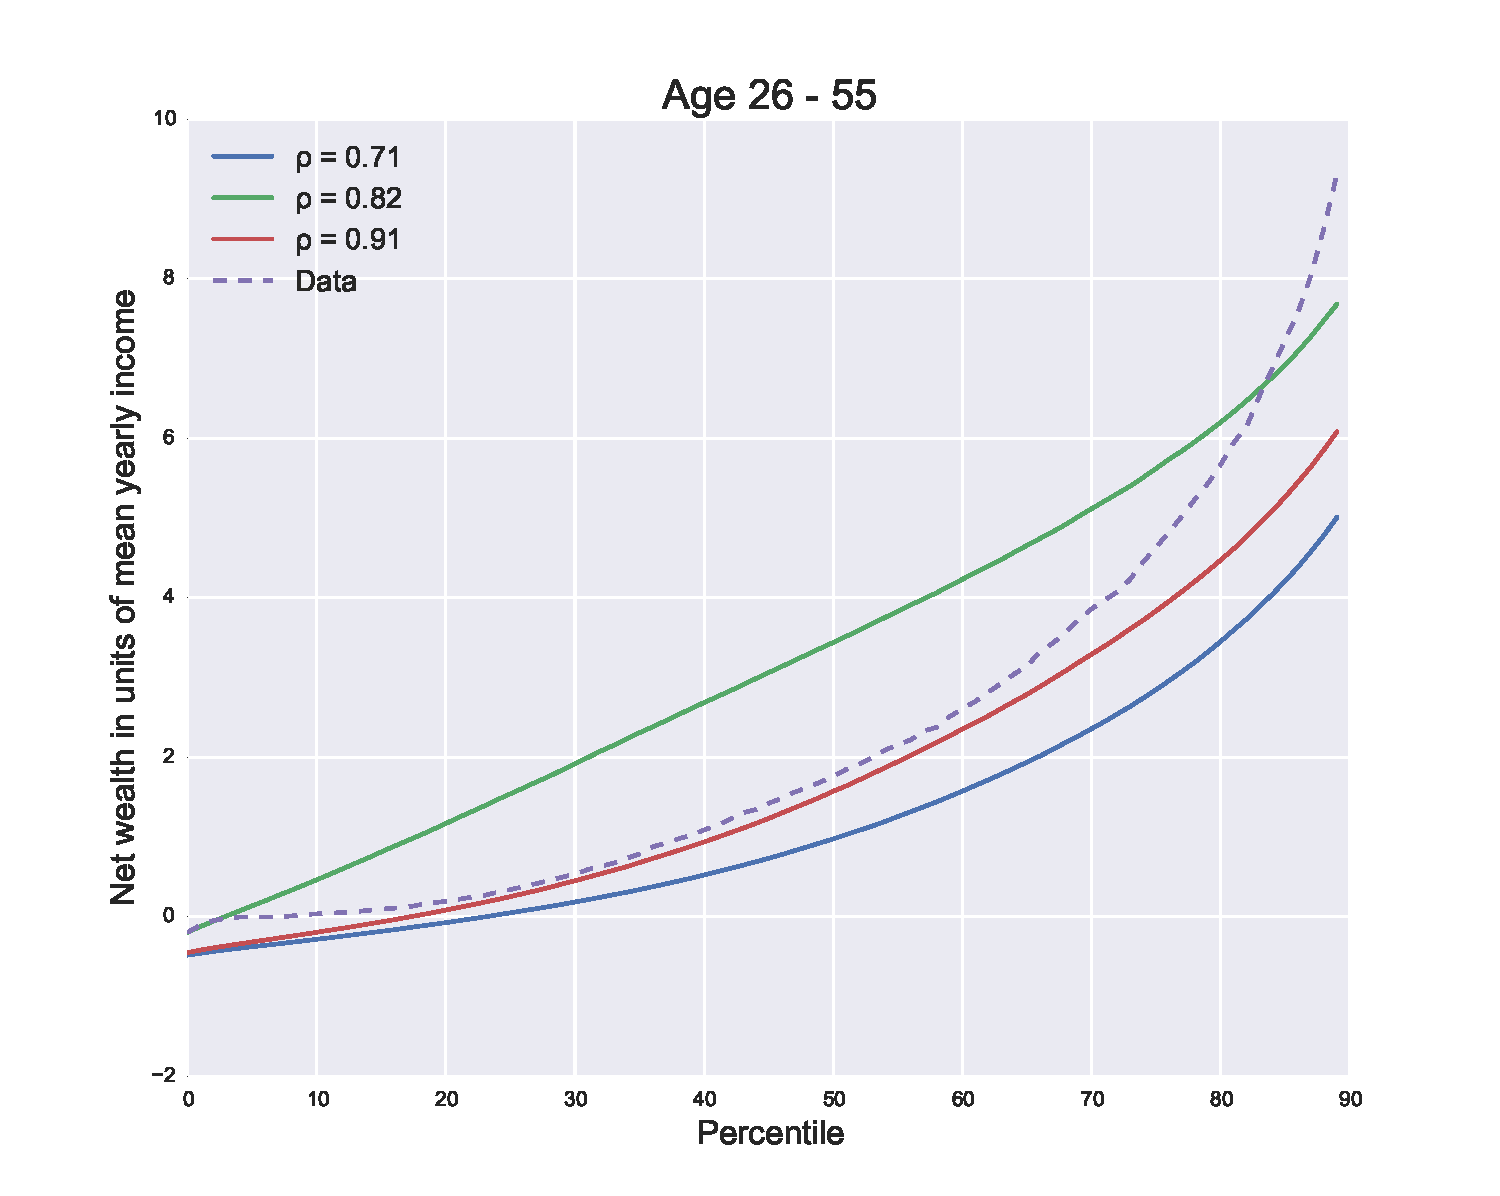
\includegraphics[width=\columnwidth]{comp_stat_rho}
\caption{Comparative statics for persistence of AR(1) component, prime age}
\label{fig:comp_stat_rho}
\end{figure}

\begin{figure}
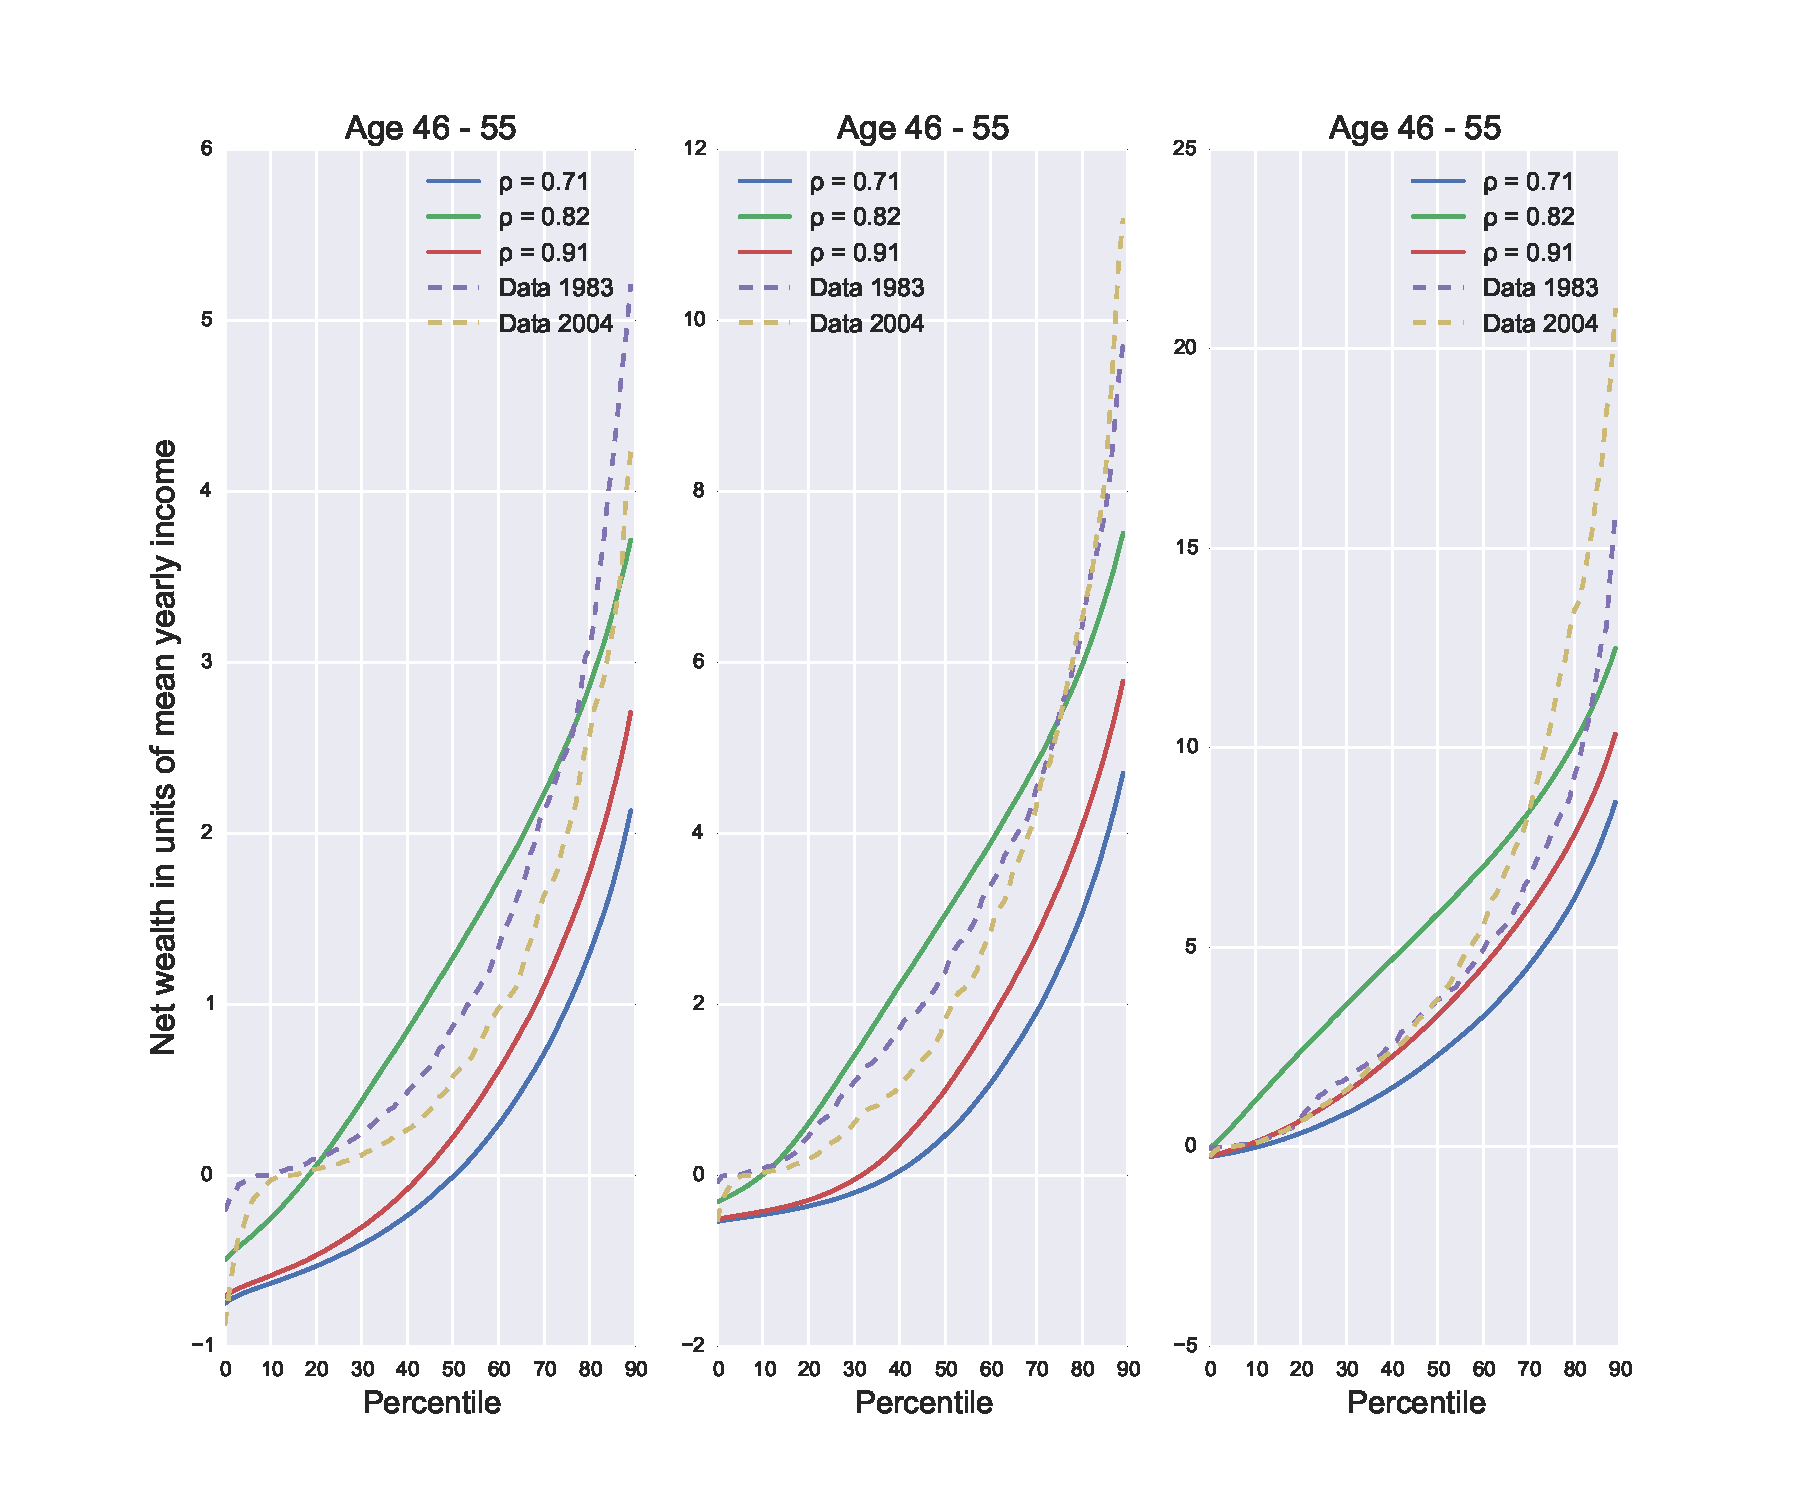
\includegraphics[width=\columnwidth]{comp_stat_rho_agedetail}
\caption{Comparative statics for persistence of AR(1) component, by age groups}
\label{fig:comp_stat_rho_agedetail}
\end{figure}

\begin{figure}
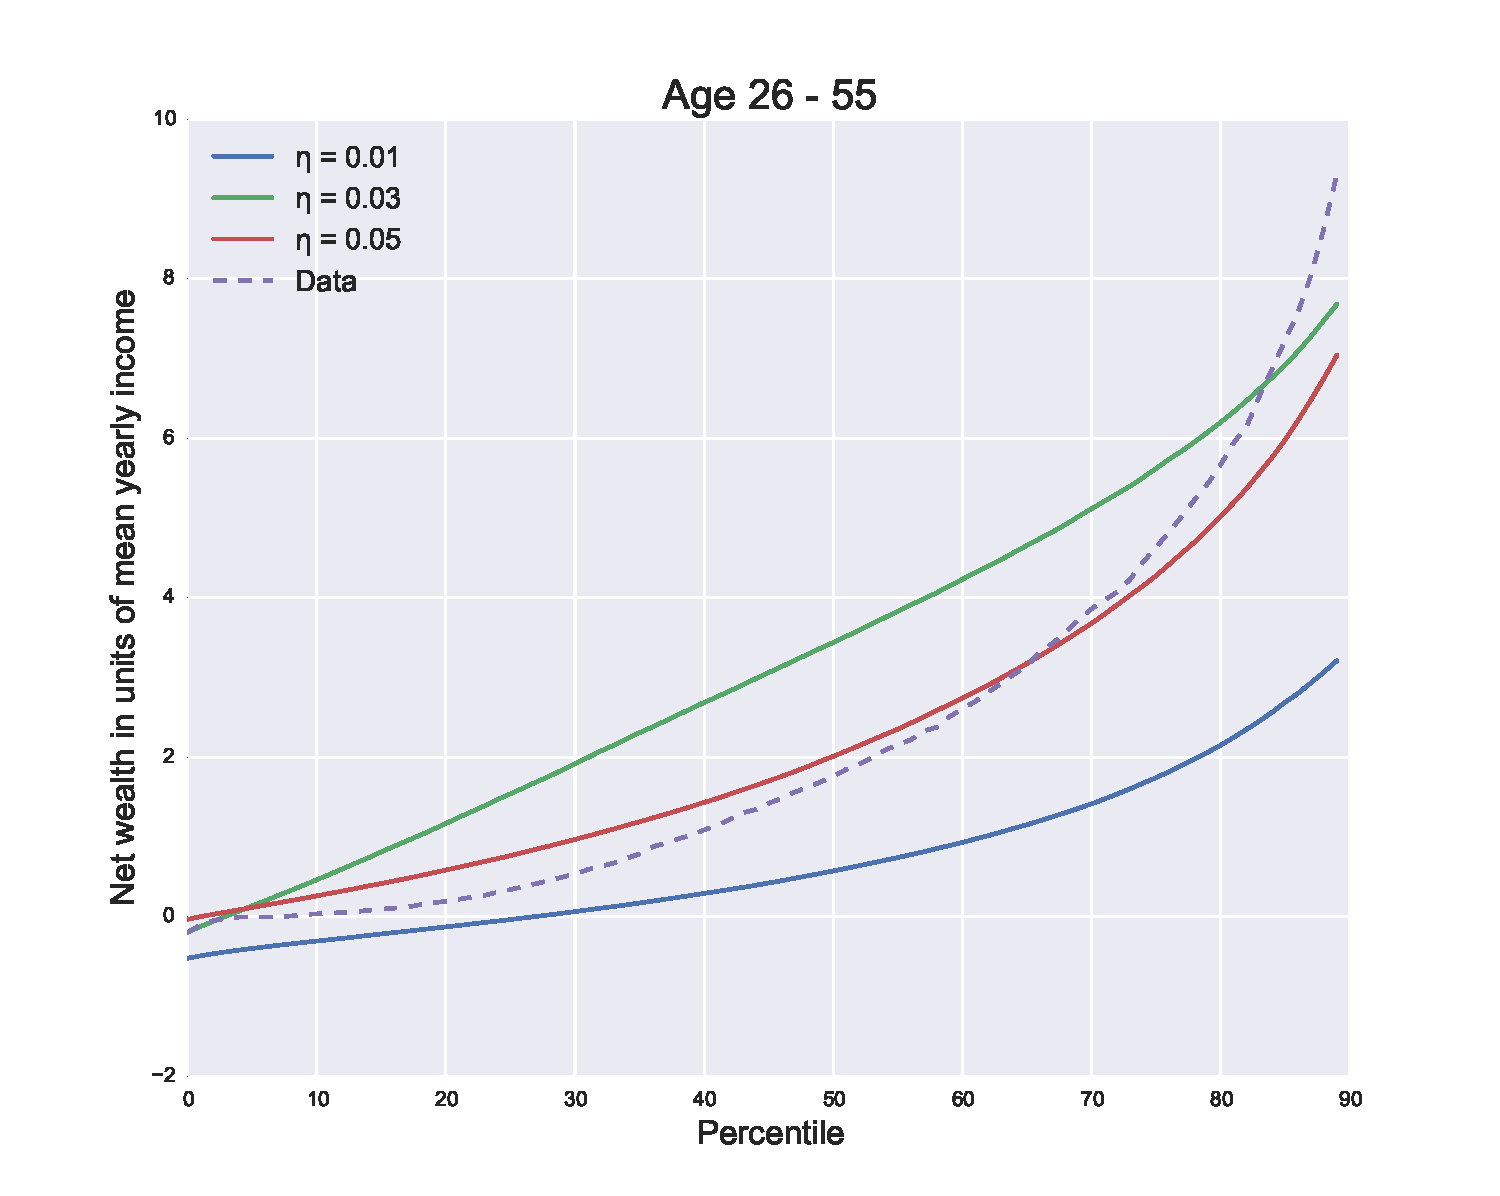
\includegraphics[width=\columnwidth]{comp_stat_eta}
\caption{Comparative statics for innovation variance of persistent shock, prime age}
\label{fig:comp_stat_eta}
\end{figure}

\begin{figure}
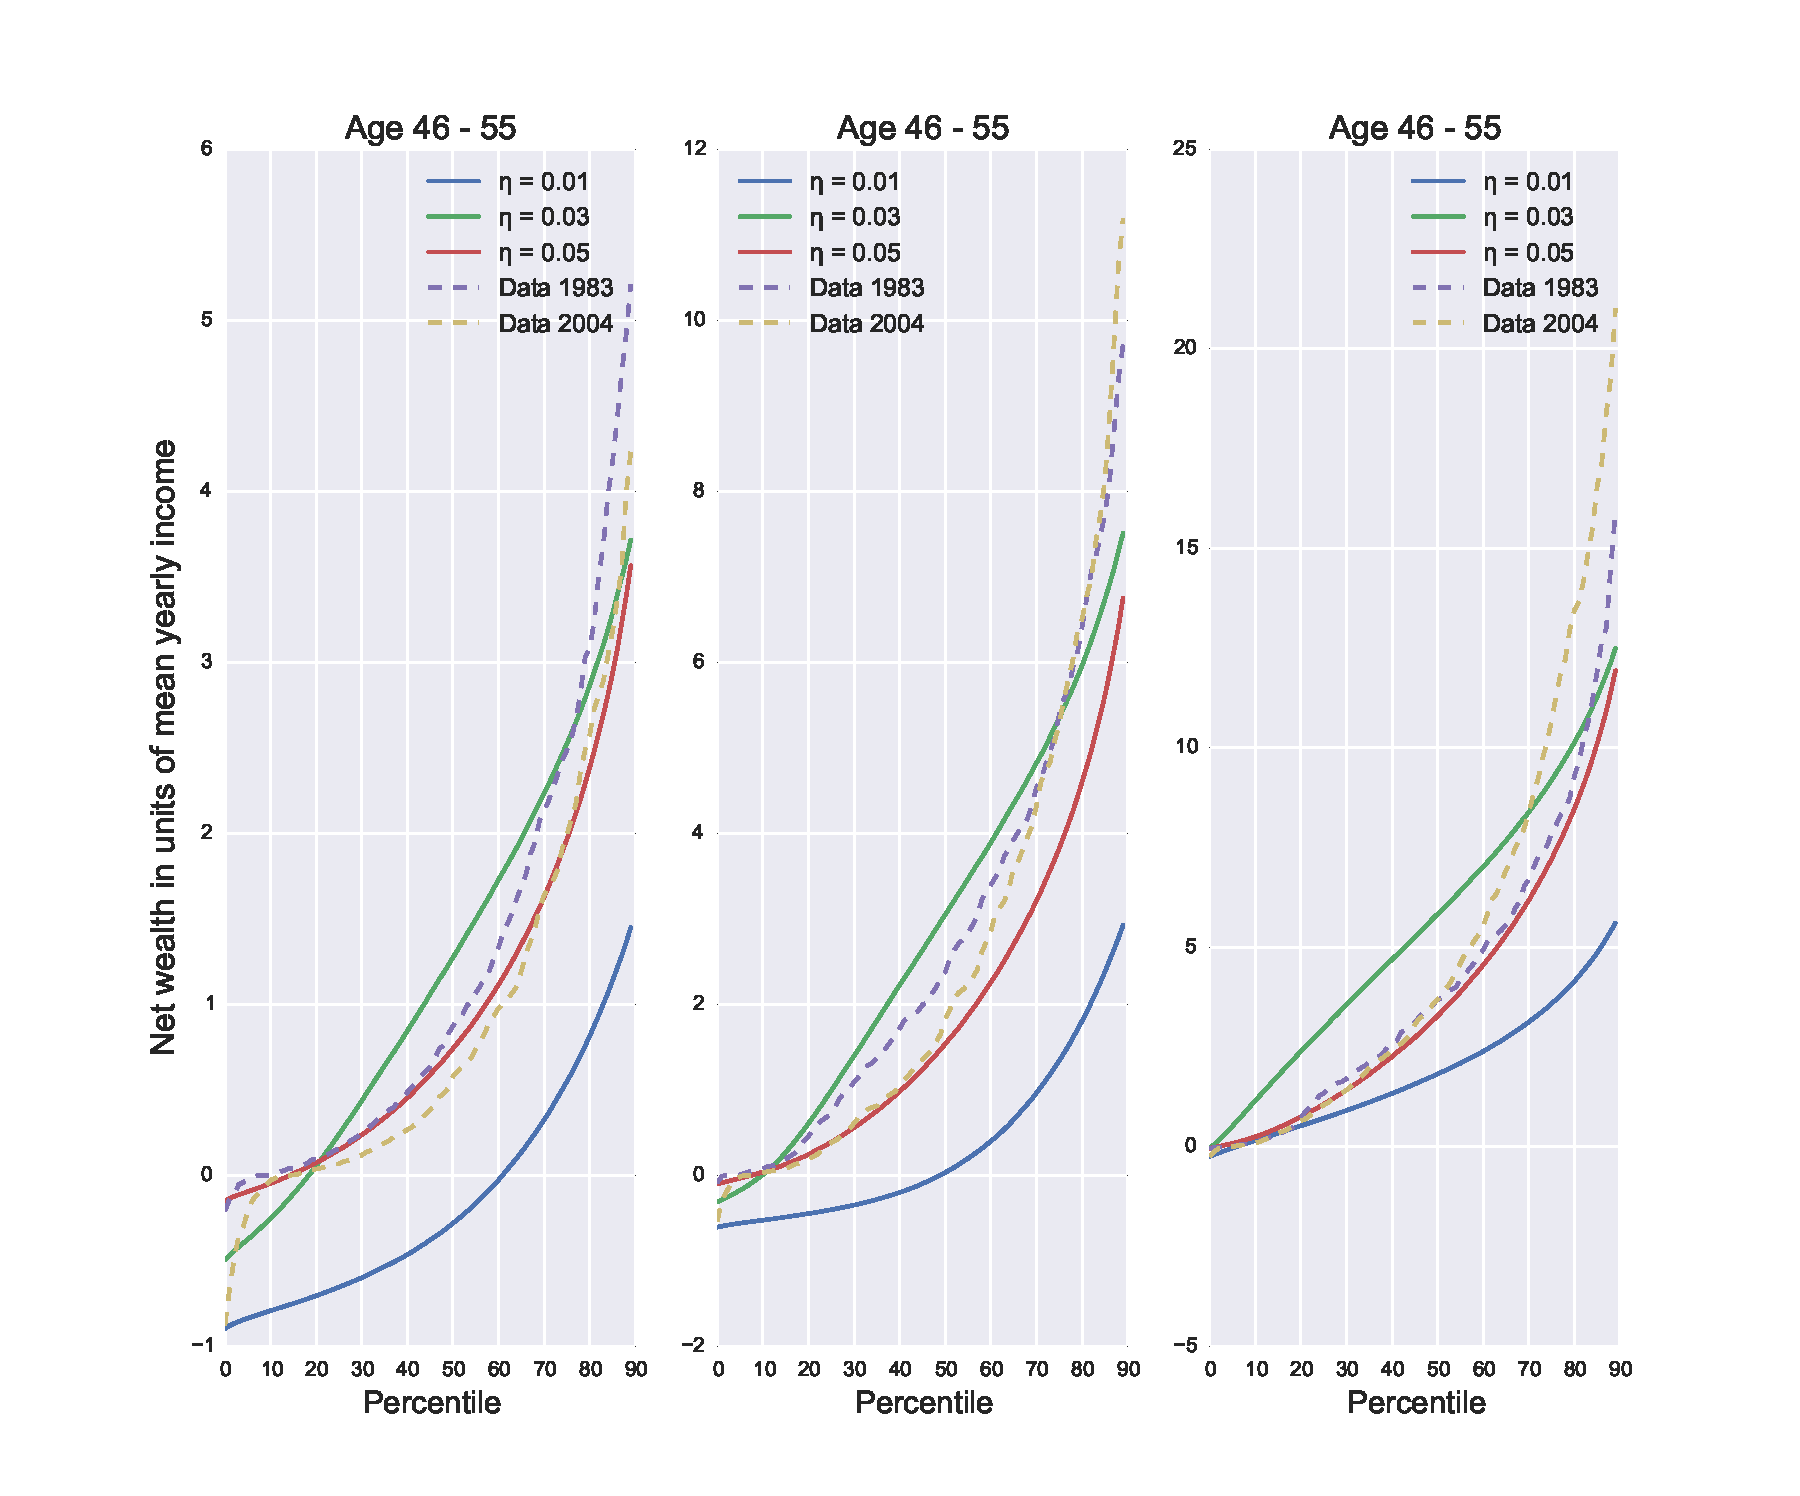
\includegraphics[width=\columnwidth]{comp_stat_eta_agedetail}
\caption{Comparative statics for innovation variance of persistent shock, by age groups}
\label{fig:comp_stat_eta_agedetail}
\end{figure}

\begin{figure}
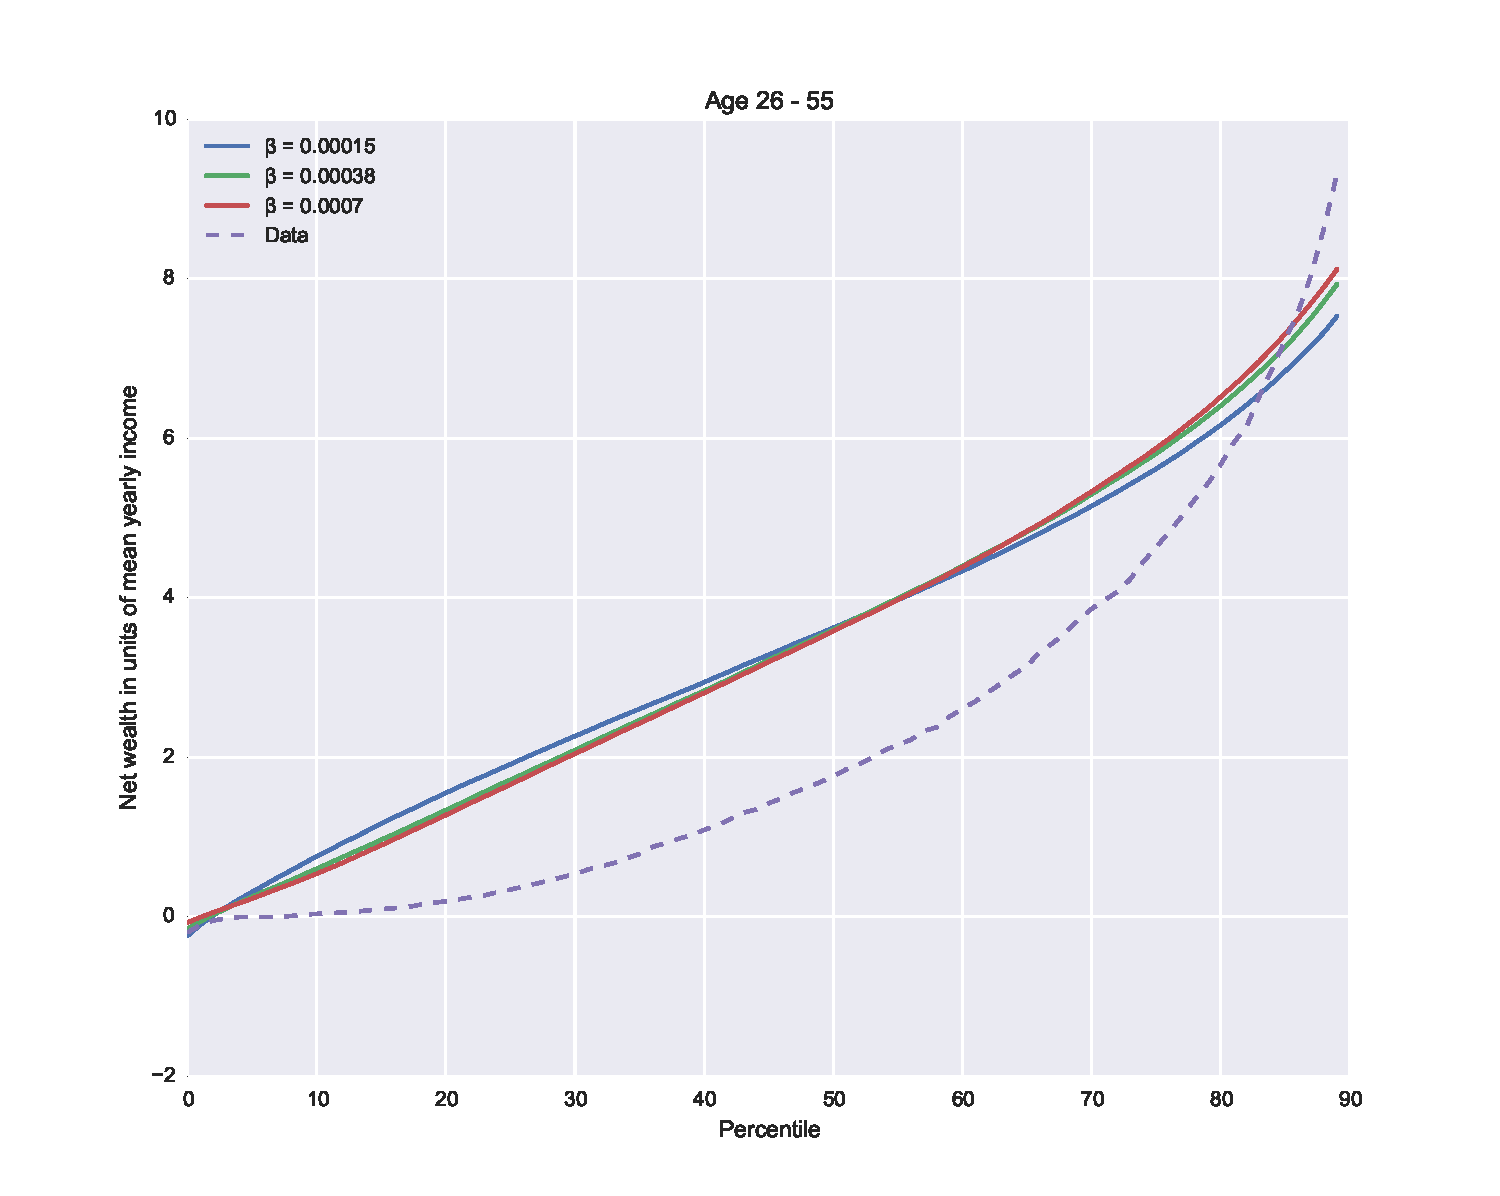
\includegraphics[width=\columnwidth]{comp_stat_beta}
\caption{Comparative statics for variance of individual-specific growth rates, prime age}
\label{fig:comp_stat_beta}
\end{figure}

\begin{figure}
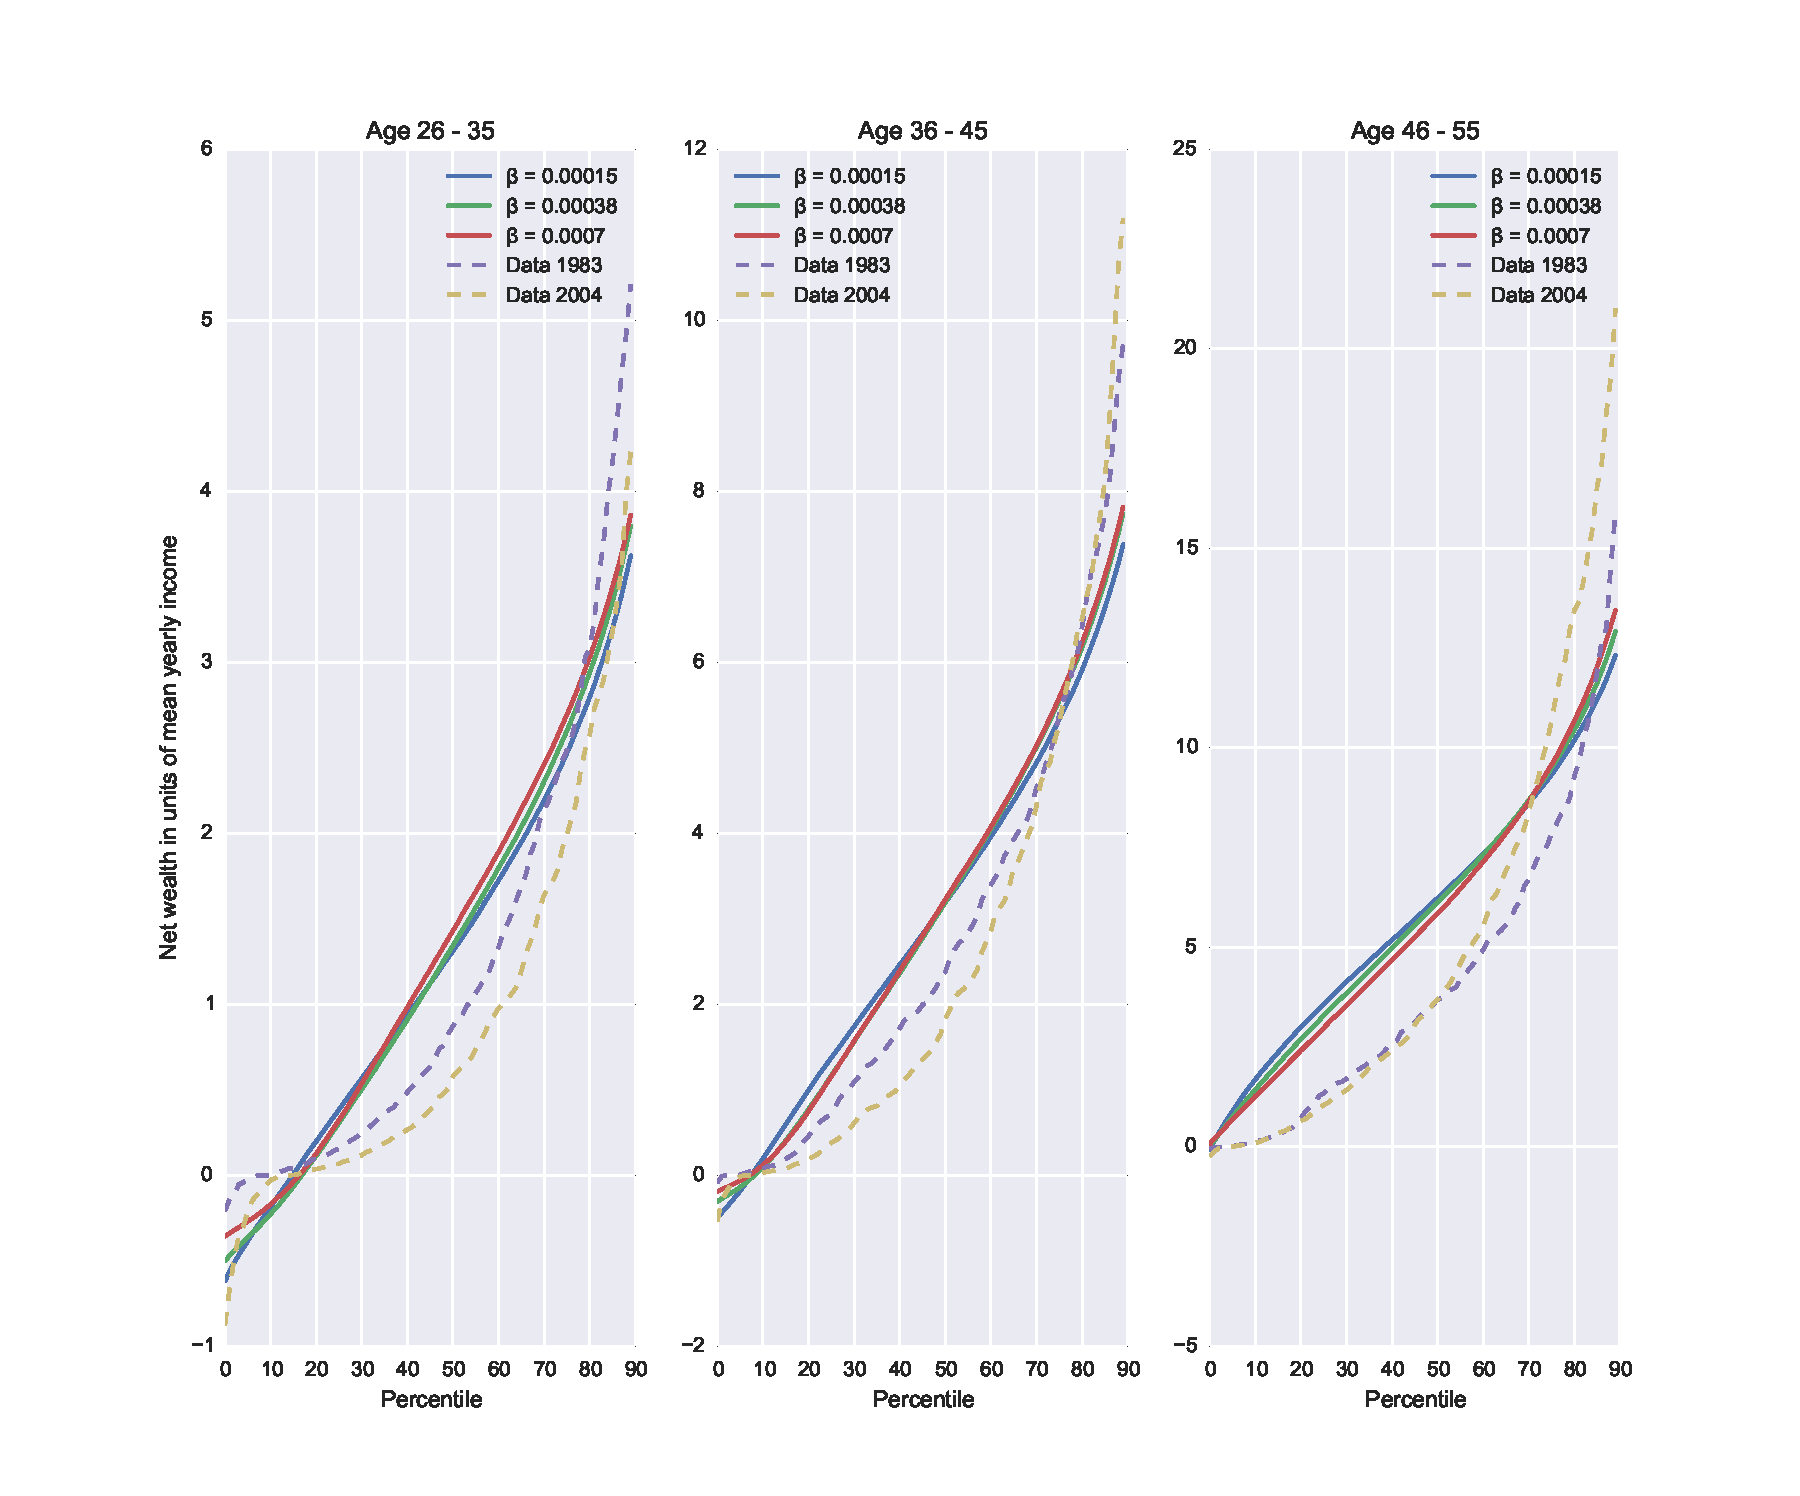
\includegraphics[width=\columnwidth]{comp_stat_beta_agedetail}
\caption{Comparative statics for variance of individual-specific growth rates, by age groups}
\label{fig:comp_stat_beta_agedetail}
\end{figure}


\section{The role of initial beliefs}
One question when working with beliefs is obviously how initial beliefs are 
derived. While the model so far had agents starting with random beliefs centred
around their individual-specific true parameter, and we have discussed the role
of uncertainty induced by learning, we will now briefly consider situations in 
which the initial beliefs are systematically incorrect. Of course, with an 
appropriately chosen set of initial beliefs, the model can be made to produce 
almost any desired result, so that we will only consider two situations which 
are at least supported by anecdotal evidence. The first very simple experiment
is done under the assumption that agents suffer from overconfidence regarding
their own economic fortune. There are a host of studies that offer support for 
the view that people are too optimistic about their future earnings potential,
e.g. a Gallup poll by \citet{Moore2003} in which half of all respondents aged
18 to 29 state that they regard it very or at least somewhat likely to be rich
in the future, with the median figure for expected yearly income and wealth cited at
\$120,000 and \$1 million, respectively. Of course it is questionable whether 
actual economic choices would be based on a vague belief about the indefinite 
future\footnote{Another constraint on this is that these beliefs would require
large amounts of borrowing in the present, for which optimistic people would have
to find lenders who share their beliefs.}, we can use our model to assess what 
would happen if people would indeed act on them. Figure \ref{fig:optimisticbeta}
shows the wealth distribution that obtains if all agents start with a belief 
that is one percentage point above their original initial belief. The results
are not as striking as one might have expected, with the entire wealth distribution
apart from the lowest percentile, which is constrained in any case, being shifted
down, albeit not by much.

The second scenario under consideration is related to the shifts in the US 
income distribution happening throughout the 80s and 90s. As has been well documented,
wage inequality experienced a secular rise during this period, with top incomes
surging, while incomes at the bottom of the distribution saw their growth rates
fall. To the extent that these changes were unobserved by agents contemporaneously,
and happened through changes in the idiosyncratic growth rates, they might have
biased beliefs of agents entering the labour market, if they form their beliefs
based on past observations of income growth for people in similar places in the 
wealth distribution. To capture a stylised version of this process in the model
we will solve the model assuming that those agents in the upper quintile of the 
true distribution of $\beta$
start life with a belief one percentage point below their original initial belief,
those in percentiles 60 to 80 half a percentage point lower, those in percentiles
20 to 40 half a percentage point higher, and those in the bottom quintile one 
percentage point higher. The results in figure \ref{fig:experiment} show 
a tilting of the wealth distribution, with agents at the upper end accumulating
more wealth, since they ascribe a larger part of their good fortune to permanent
shocks given that they systematically underestimate their deterministic growth
rate. At the same time, more agents at the lower end of the distribution are 
constrained, as they expect higher future income growth than will actually 
materialise. These changes in the wealth distribution are consistent with the
observed increase in wealth inequality that followed the increase in income 
inequality in the 1980s and 90s (as discussed in \citet{Iacoviello2008}) and 
could form the basis of a demand-driven expansion of household debt at the lower
end of the income distribution. Indeed, rising income inequality is often cited as 
a prime reason for the increase in household indebtedness (see e.g. \citet{Rajan2011},
\citet{SaezZucman2014}, or, for a more heterodox treatment, \citet{BarbaPivetti2009}),
although from the standpoint of a standard life-cycle model of consumption and 
savings this link should be absent, given that recent work based on Social 
Security records shows virtually the entire increase in income inequality to
be due to permanent, rather than transitory shocks, which should result in 
changes in consumption, rather than wealth inequality. One possibility for 
permanent changes in the income distribution not to immediately filter through
to the consumption distribution could then, according to our model, be hysteresis
in belief formation of agents entering the labour market at different points
of the income distribution.

\begin{figure}
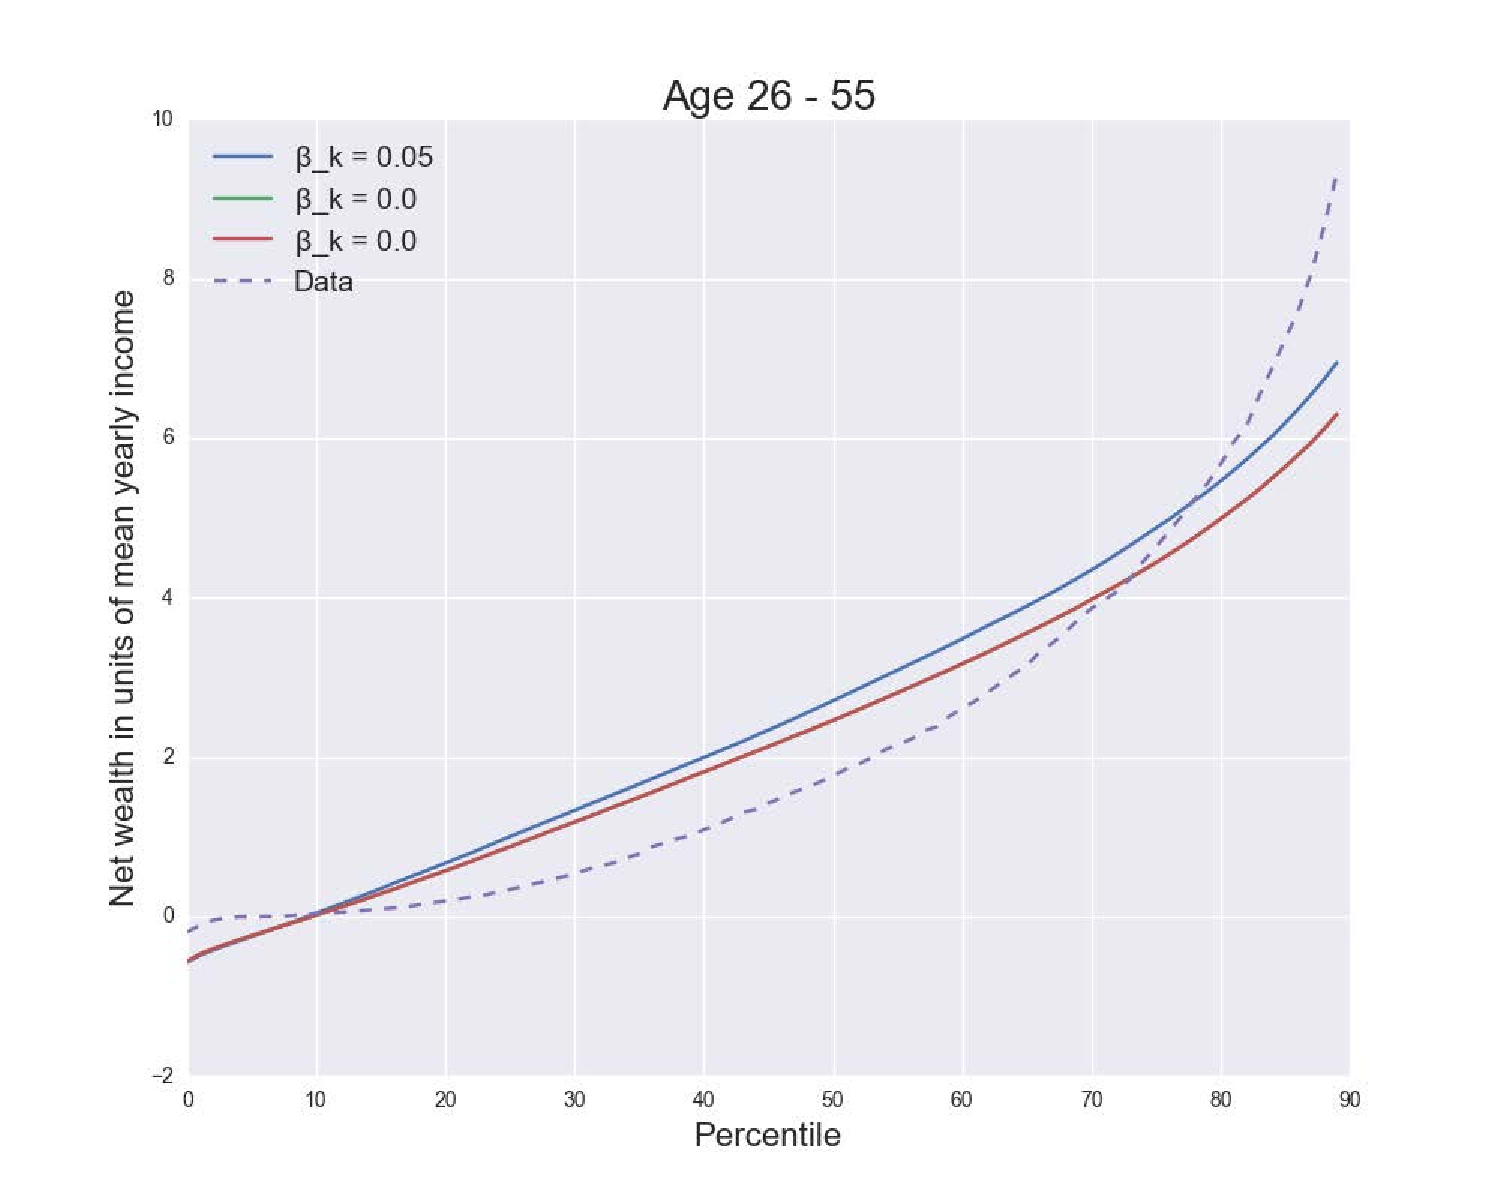
\includegraphics[width=\columnwidth]{optimisticbeta}
\caption{Effects of optimistic initial beliefs}
\label{fig:optimisticbeta}
\end{figure}

\begin{figure}
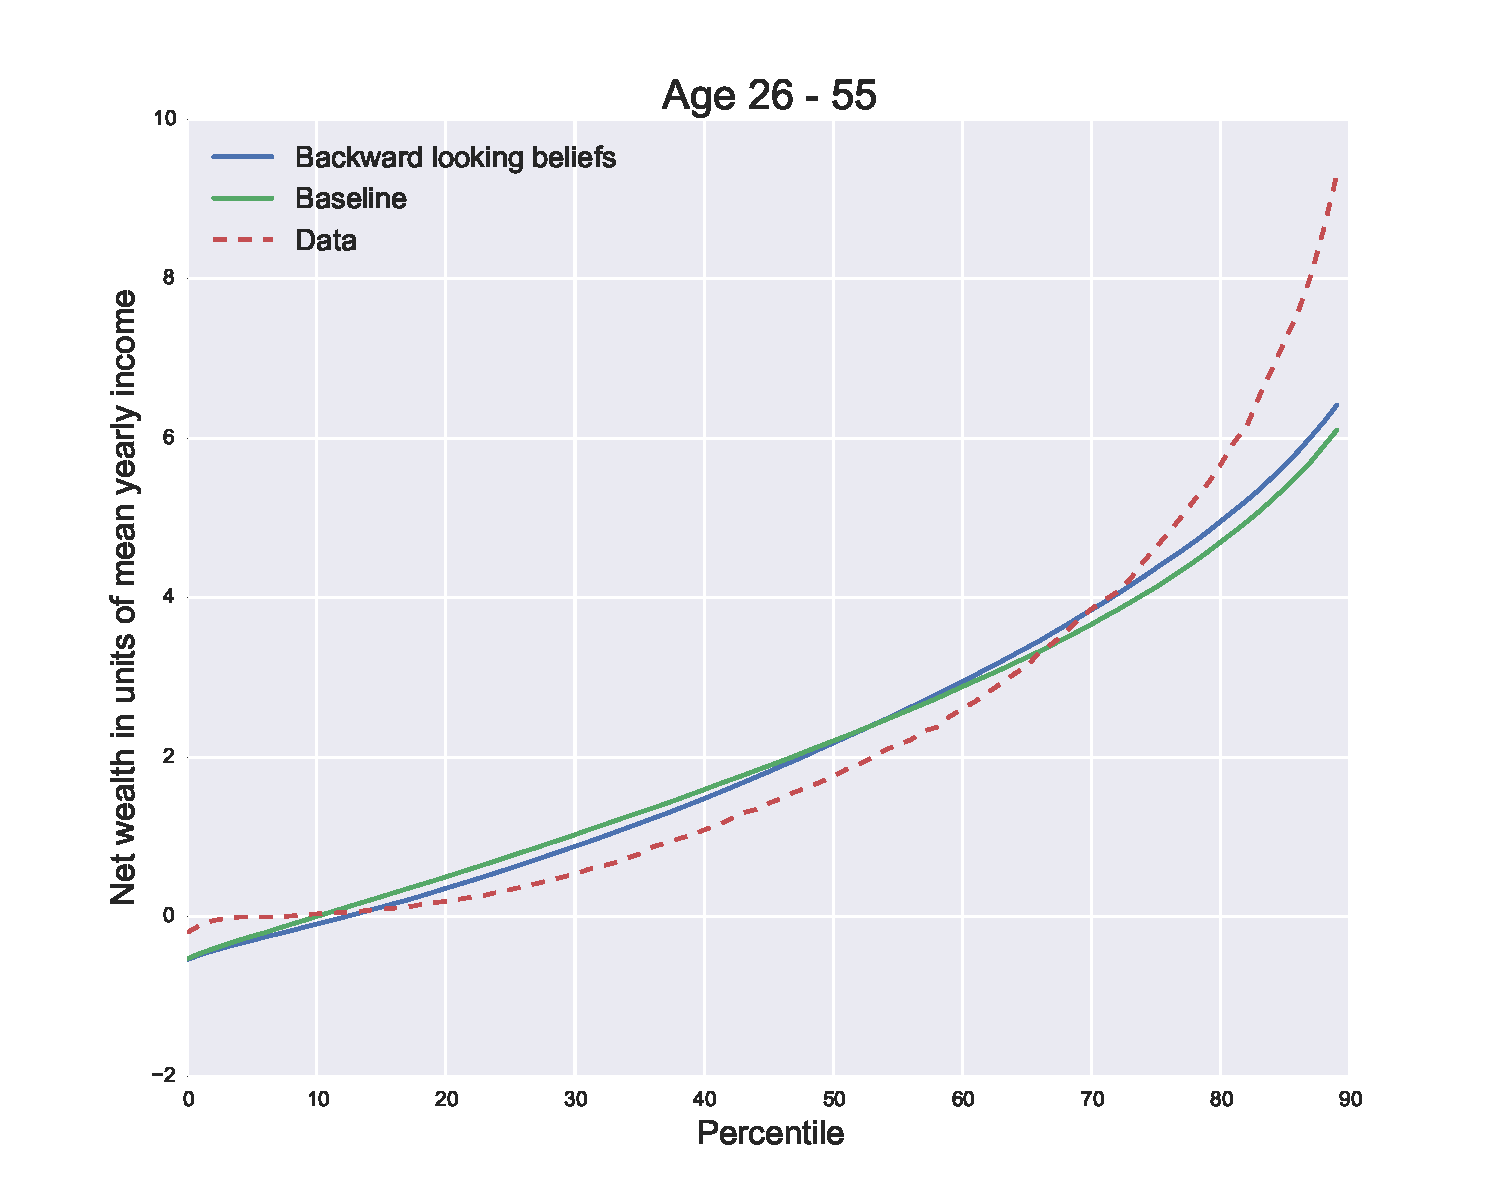
\includegraphics[width=\columnwidth]{experiment}
\caption{Effects of beliefs based on previous income growth rates}
\label{fig:experiment}
\end{figure}

\section{Incorporating disaster risk}
Figure \ref{fig:disaster} shows the effect of including the subjective possibility 
of a zero income realisation on savings profiles. It is noted that the actual 
underlying income process is not altered, so that while agents expect a zero 
income realisation with probability $\xi$ in each period, it actually never 
materialises, so that the income histories in this model economy are exactly 
the same as in our previous examples. 
\begin{figure}
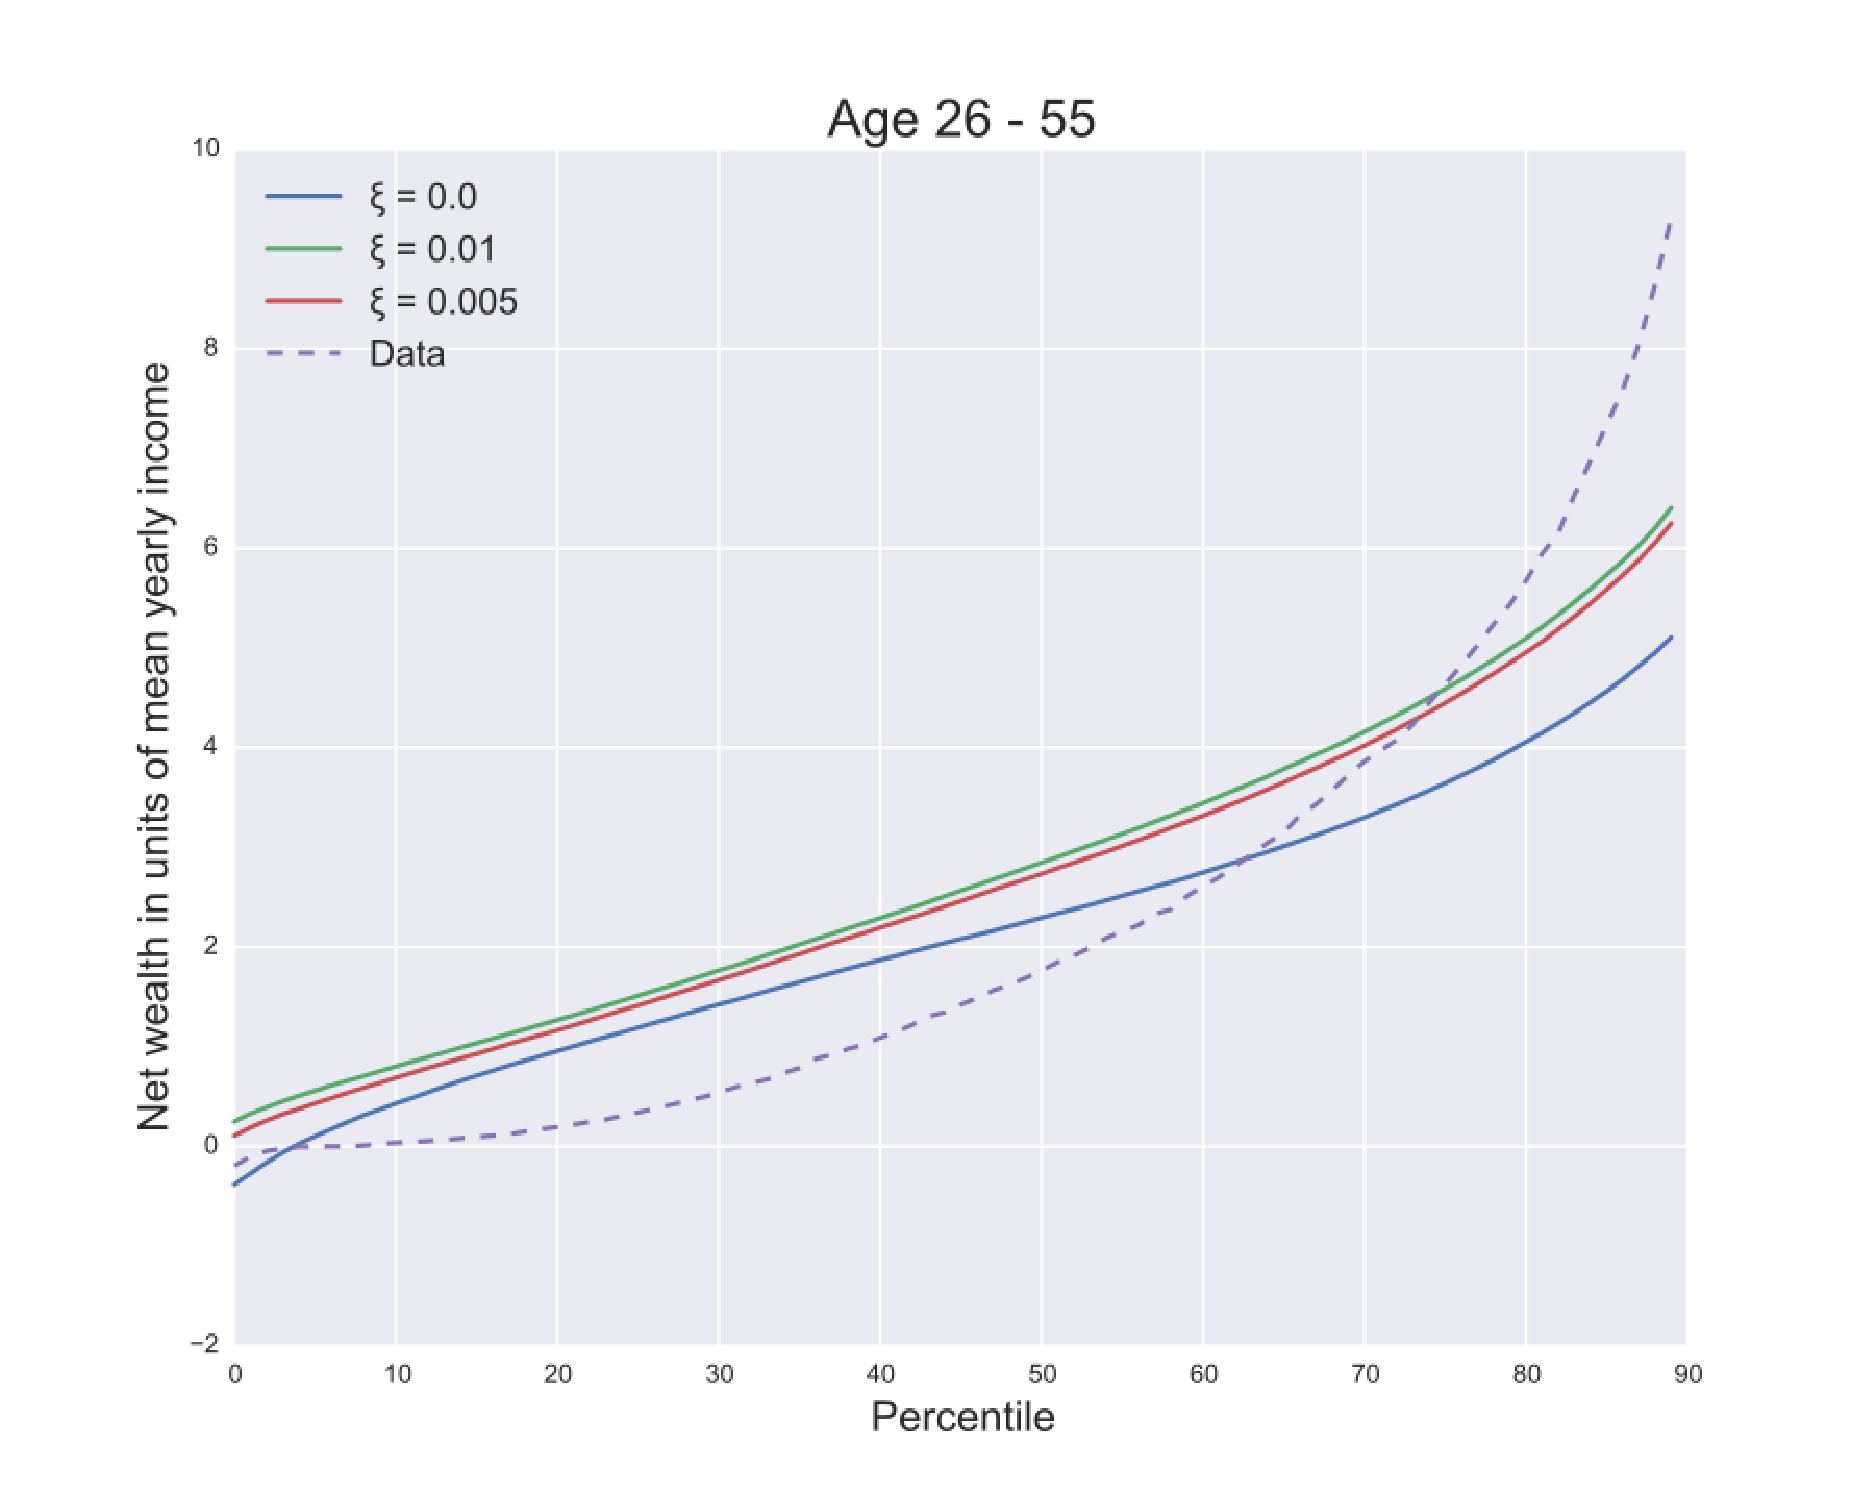
\includegraphics[width=\columnwidth]{disaster}
\caption{Effects of subjective belief about probability of zero income 
           realisation}
\label{fig:disaster}
\end{figure}

\section{Bequest motives}
Figure \ref{fig:bequests} shows the effect of including a bequest motive, modelled
as in e.g. \citet{KopczukLupton2007}. In this model economy, the working life 
problem is equivalent to that outlined in equation \ref{eq:bellman}, while the
retirement problem is adapted to include a positive probability of dying in 
each period (taking from U.S. mortality statistics) and utility from dying with
positive asset holdings. The household problem is:
\begin{align}\label{eq:retirement_bequest}
\max_{\{c_t\}_{t=1}^{T}} \sum_{t = 1}^{T} \delta^t (1-\zeta)u(c_t) + \zeta \kappa a_t 
\end{align}
subject to the same constraints as in equation \ref{eq:retirement}. 
Here, $\zeta$ is the age-varying probability of dying before next period, while
$\kappa$ is a constant scaling parameter measuring the importance of bequests 
relative to personal consumption. This specification implies that bequests are a 
luxury good, as the marginal utility of leaving a bequest increases in the level 
of wealth holdings. This assumption is standard in the literature on bequests.
Figure \ref{fig:bequests} shows that incorporating a bequest motive dramatically
improves the fit of the model, as it allows for a significant increase in wealth
accumulation at the top of the wealth distribution. Due to numerical instabilities
it has unfortunately not been possible to jointly estimate the $(\beta,\sigma,
\kappa)$ combination  

\begin{figure}
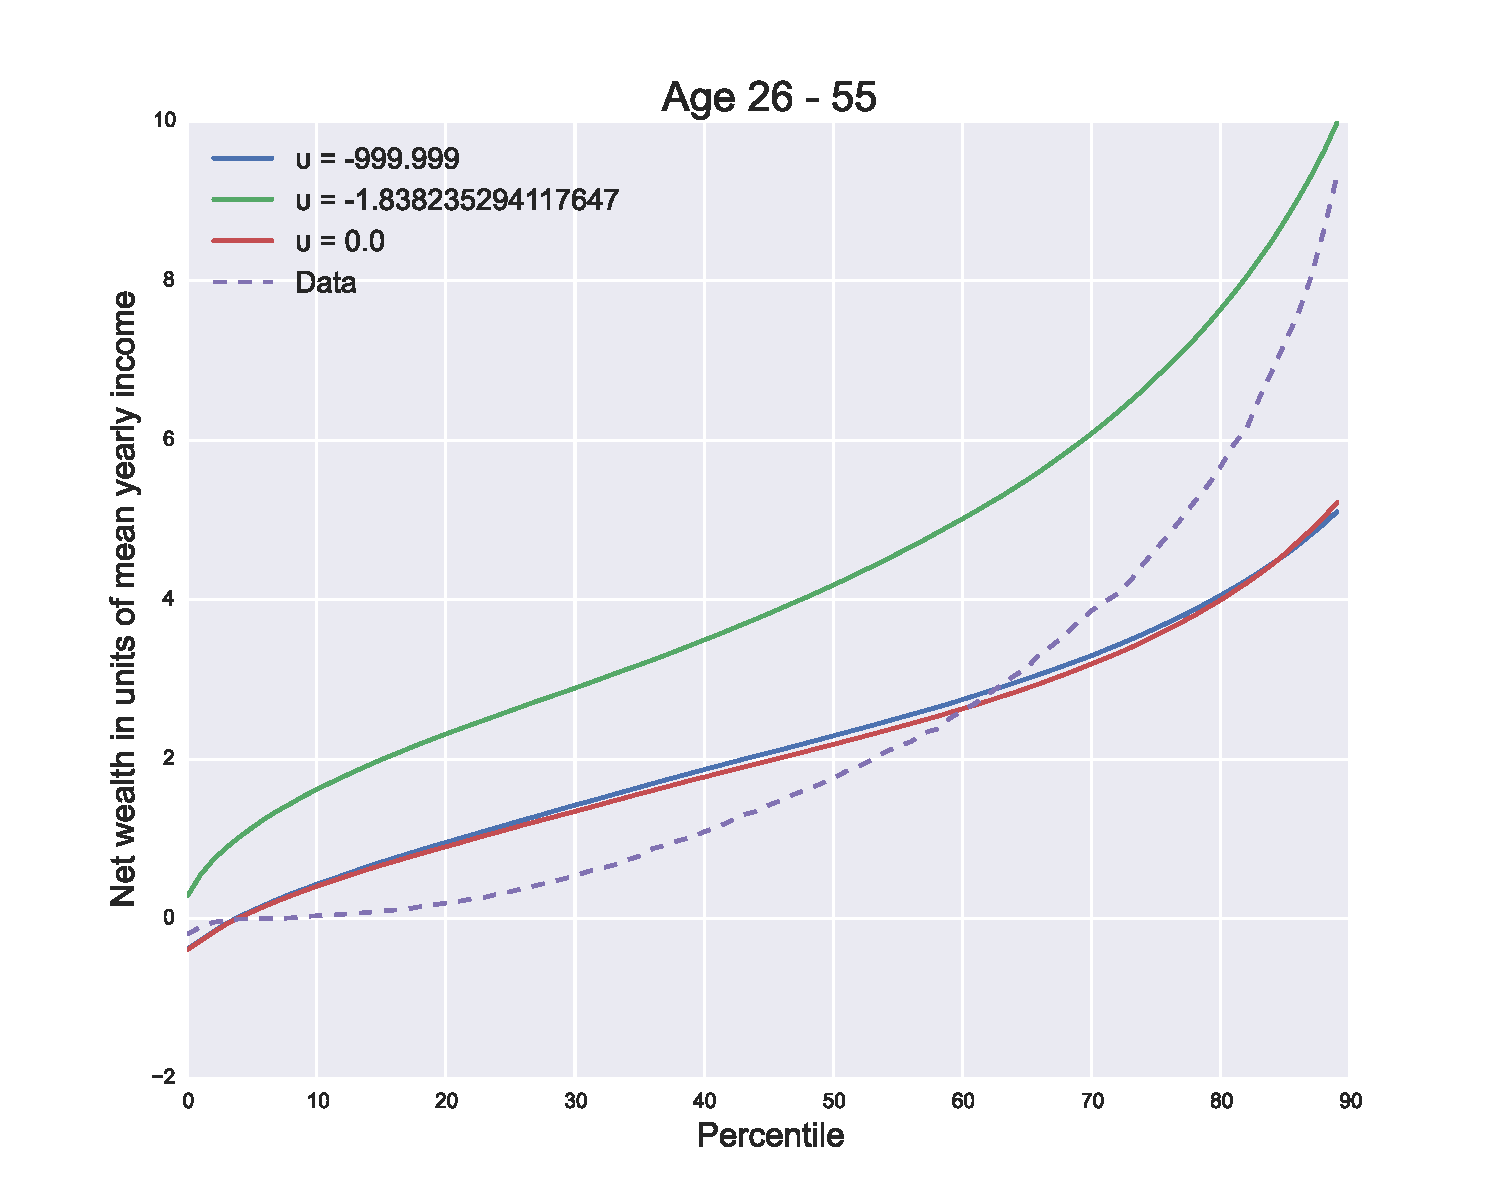
\includegraphics[width=\columnwidth]{bequest_motive}
\caption{Effects of bequest motive}
\label{fig:bequests}
\end{figure}


\section{Discussion}\label{sec:discussion}
As this chapter has shown, the learning model of heterogeneous income processes
fails in capturing the dynamics of the wealth distribution under all calibrations
derived from empirical data on income processes. Comparing the model output of 
different counterfactual parametrisations, it became clear that the main reason
behind this is not the learning mechanism itself, but the different income 
distribution and risk implied by the heterogeneous income process. To salvage 
the model, ad-hoc changes to the belief structure of agents can be made, although
at this point it becomes a bit of a free-for-all and the model can be made to
predict any pattern in the data with a suitable choice of initial beliefs.
Building on the work in this chapter, future research should consider the implications
of other more realistic income processes on the wealth distribution, to the 
extent that they can be formulated parsimoniously enough not to increase the 
computational burden beyond reason. An example would be the work by 
\citet{MeghirPistaferri2004}, who model the conditional variance of income
shocks using an ARCH model and show analytically that the addition of individual-
specific heterogeneity in the innovation variance leads to both a larger dispersion
of savings rates and higher aggregate saving. A further case of interest would be
the specification derived by \citet{GKOS2015}, which adapts the income process
used in this chapter by adding two more AR(1) components with different innovation
variances, so that households are subject to potential shocks of different 
magnitude. As the evidence points to this process being the best description 
of the income risk households are facing in reality, the implications of this
process for the wealth distribution should be investigated further. 

\section{Appendix A: Comparative statics results}

\begin{figure}
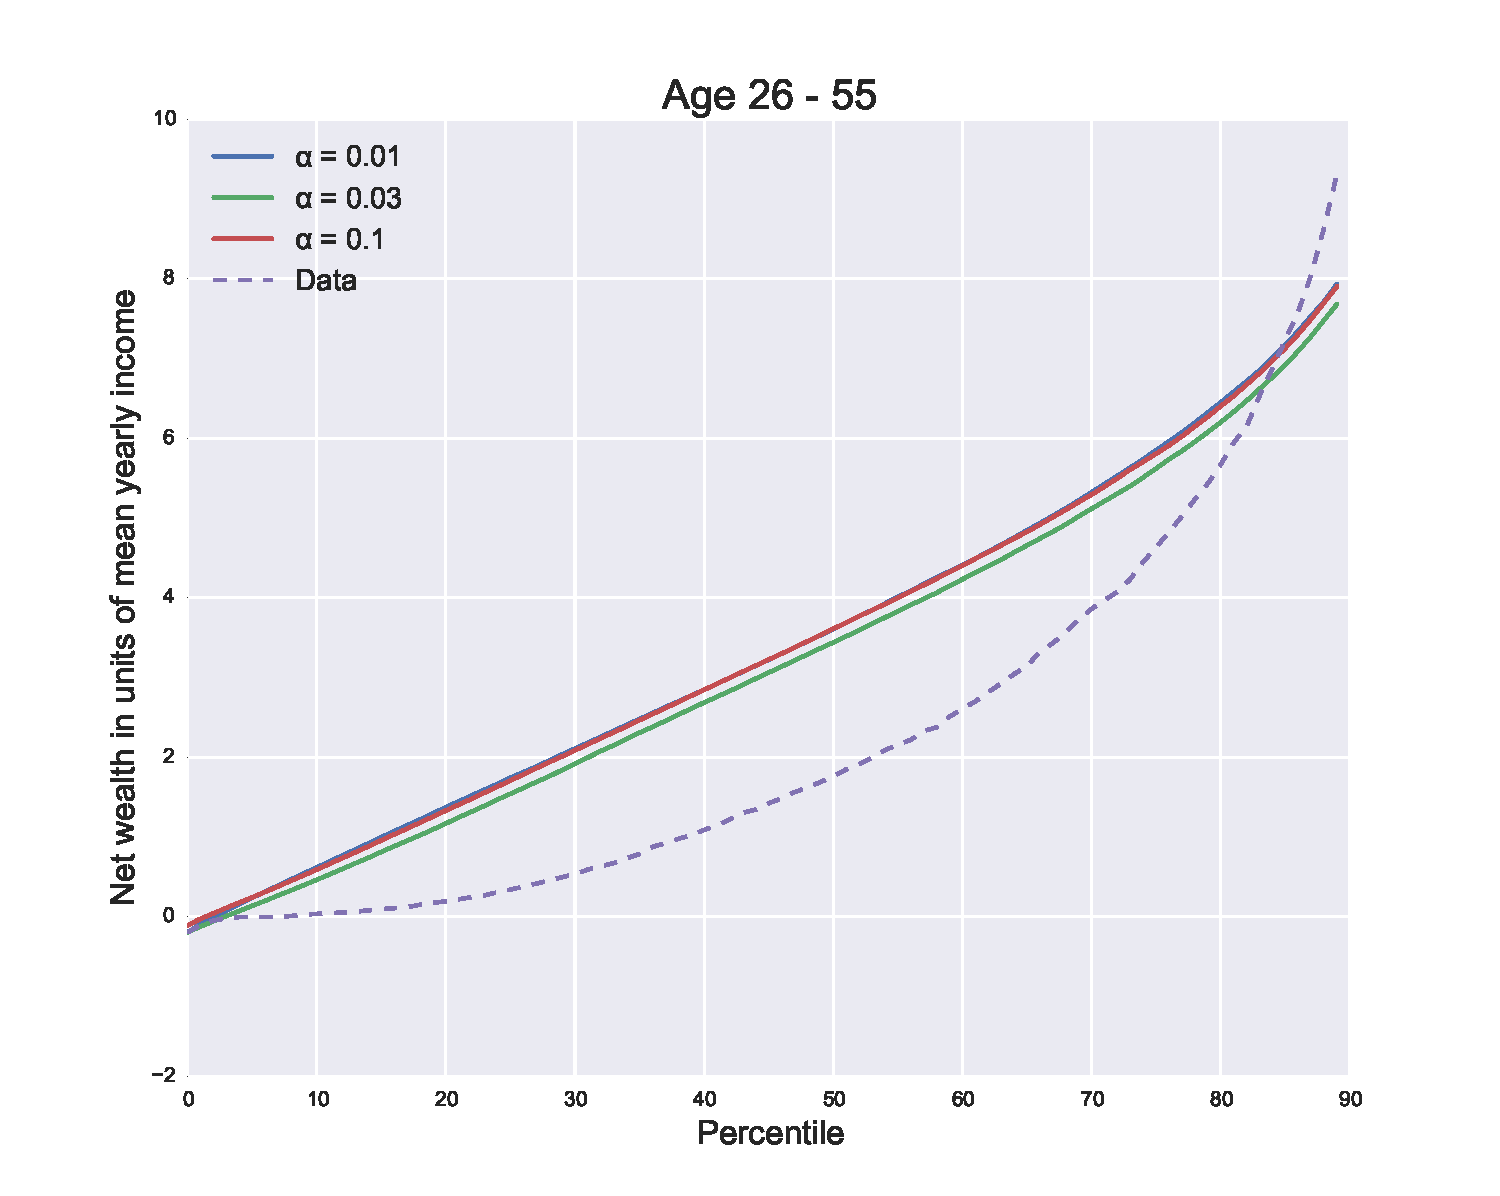
\includegraphics[width=\columnwidth]{comp_stat_alpha}
\caption{Comparative statics for variance of individual-specific intercepts, prime age}
\label{fig:comp_stat_alpha}
\end{figure}

\begin{figure}
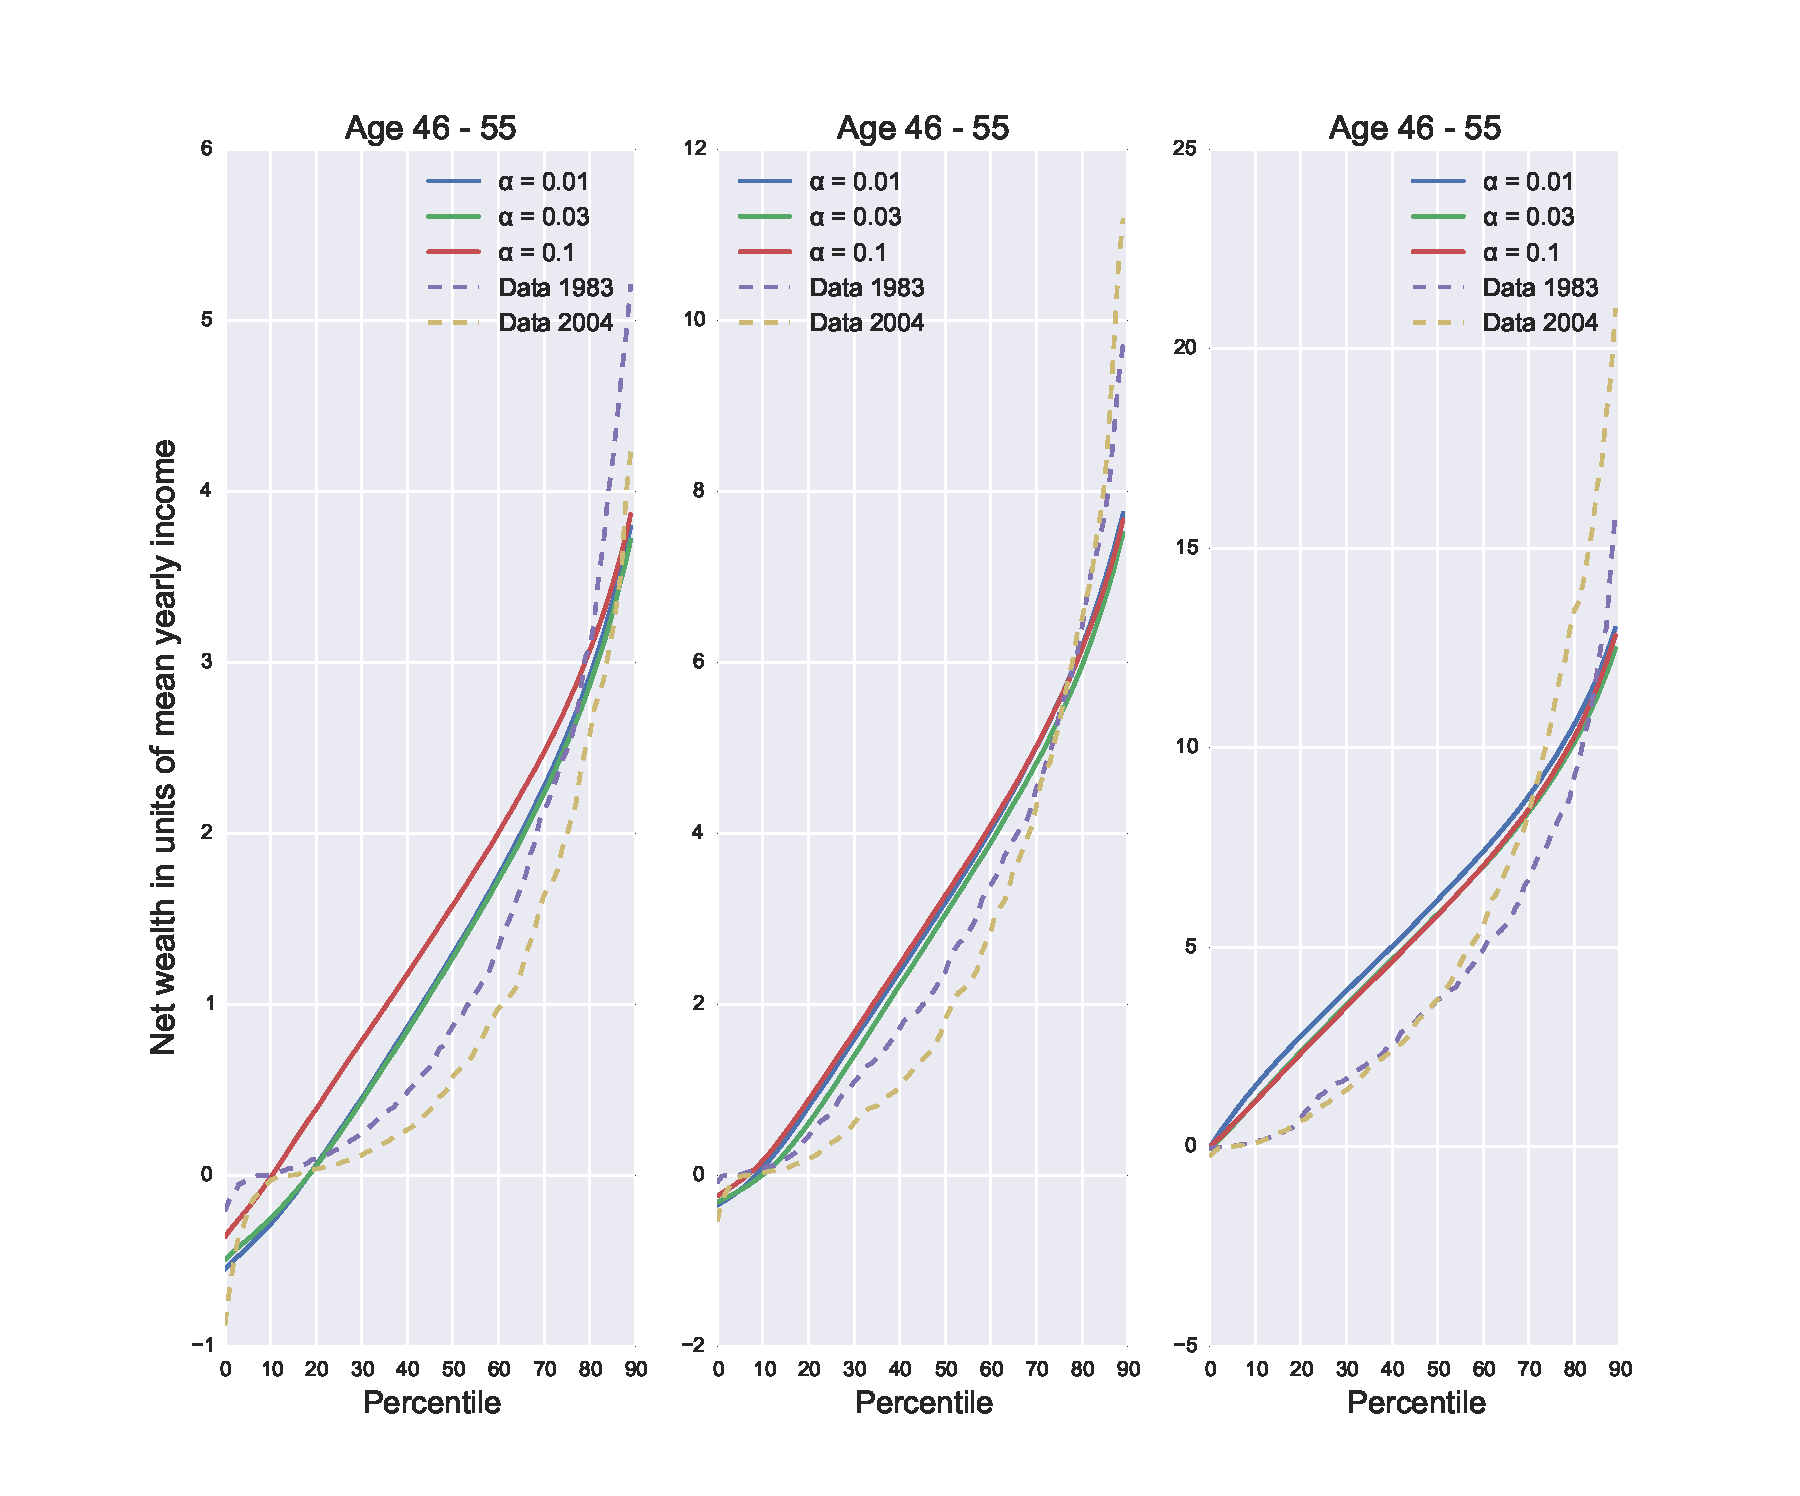
\includegraphics[width=\columnwidth]{comp_stat_alpha_agedetail}
\caption{Comparative statics for variance of individual-specific intercepts, by age group}
\label{fig:comp_stat_alpha_agedetail}
\end{figure}

\begin{figure}
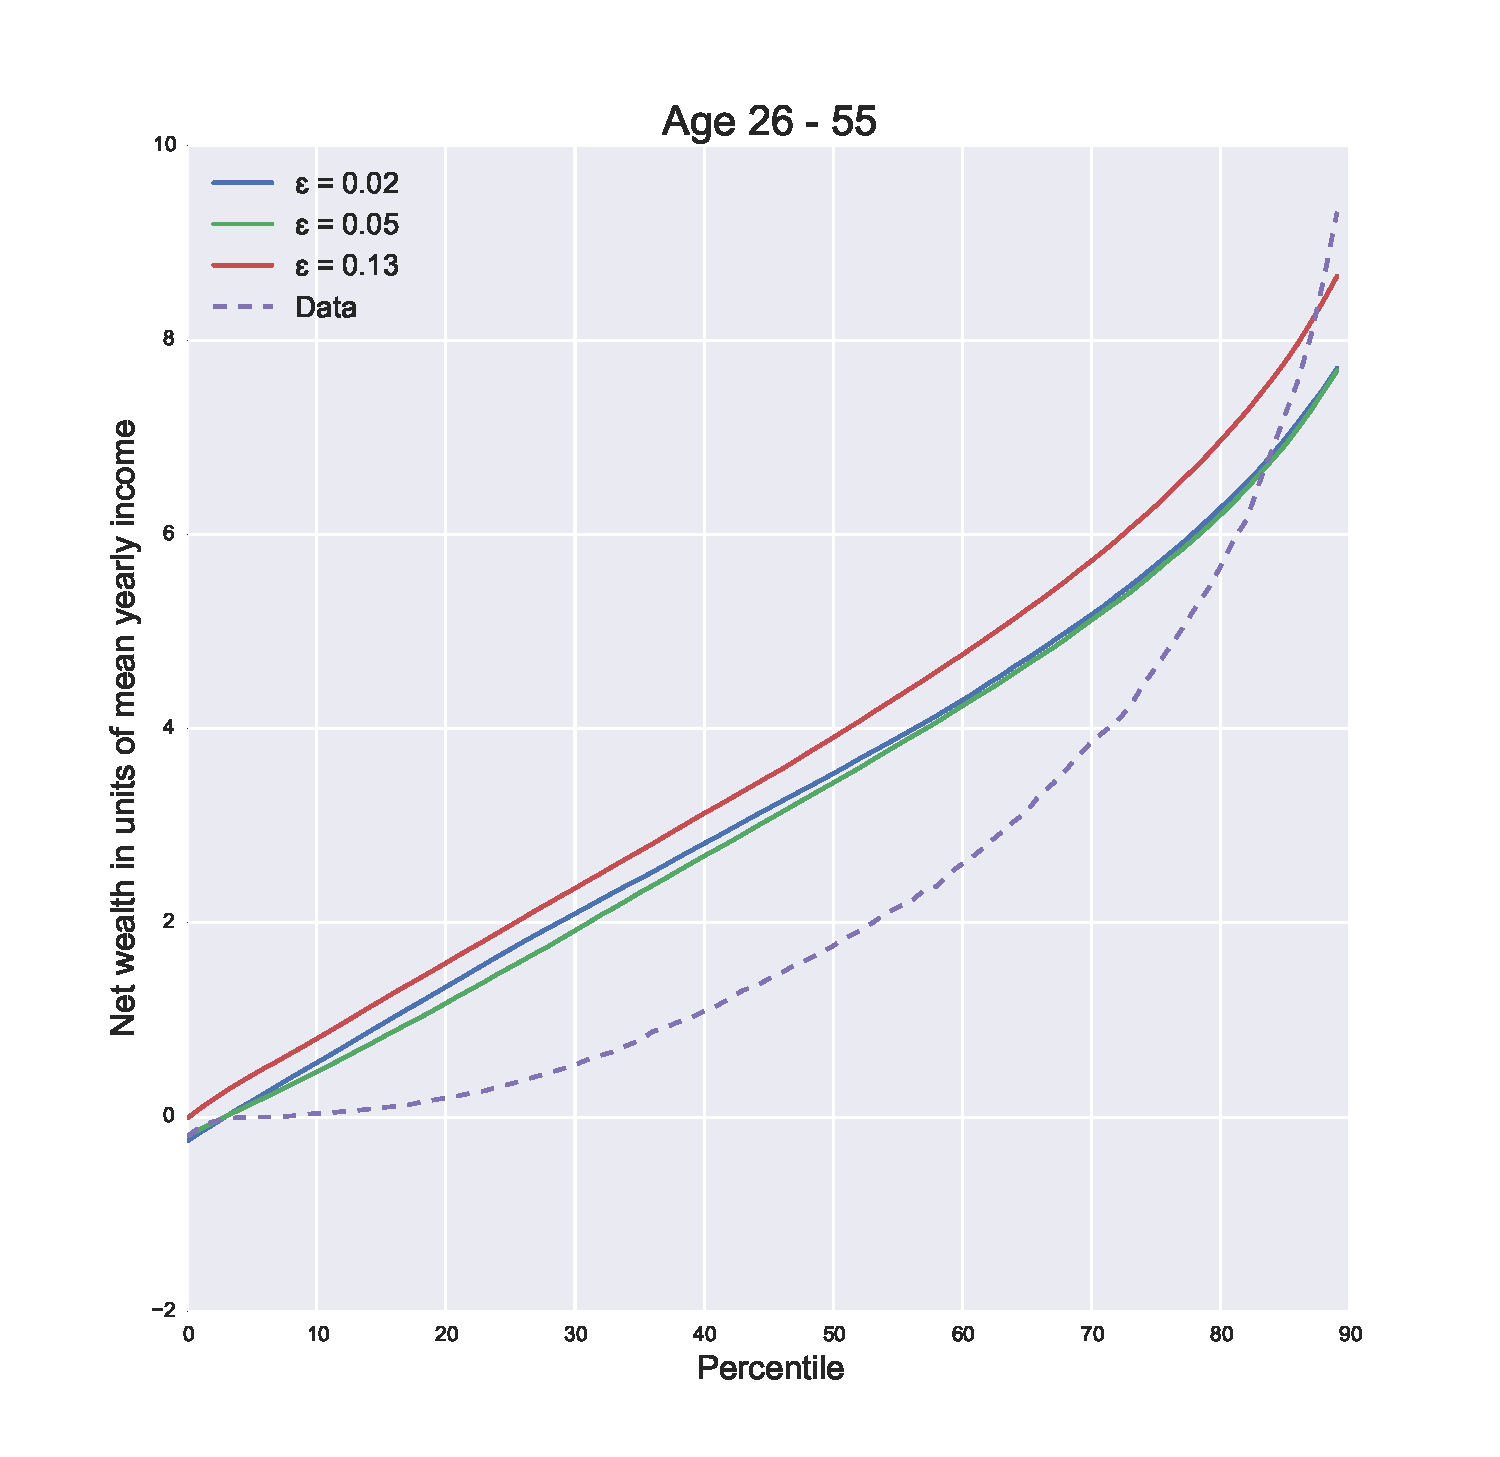
\includegraphics[width=\columnwidth]{comp_stat_eps}
\caption{Comparative statics for variance of transitory shocks, prime age}
\label{fig:comp_stat_eps}
\end{figure}

\begin{figure}
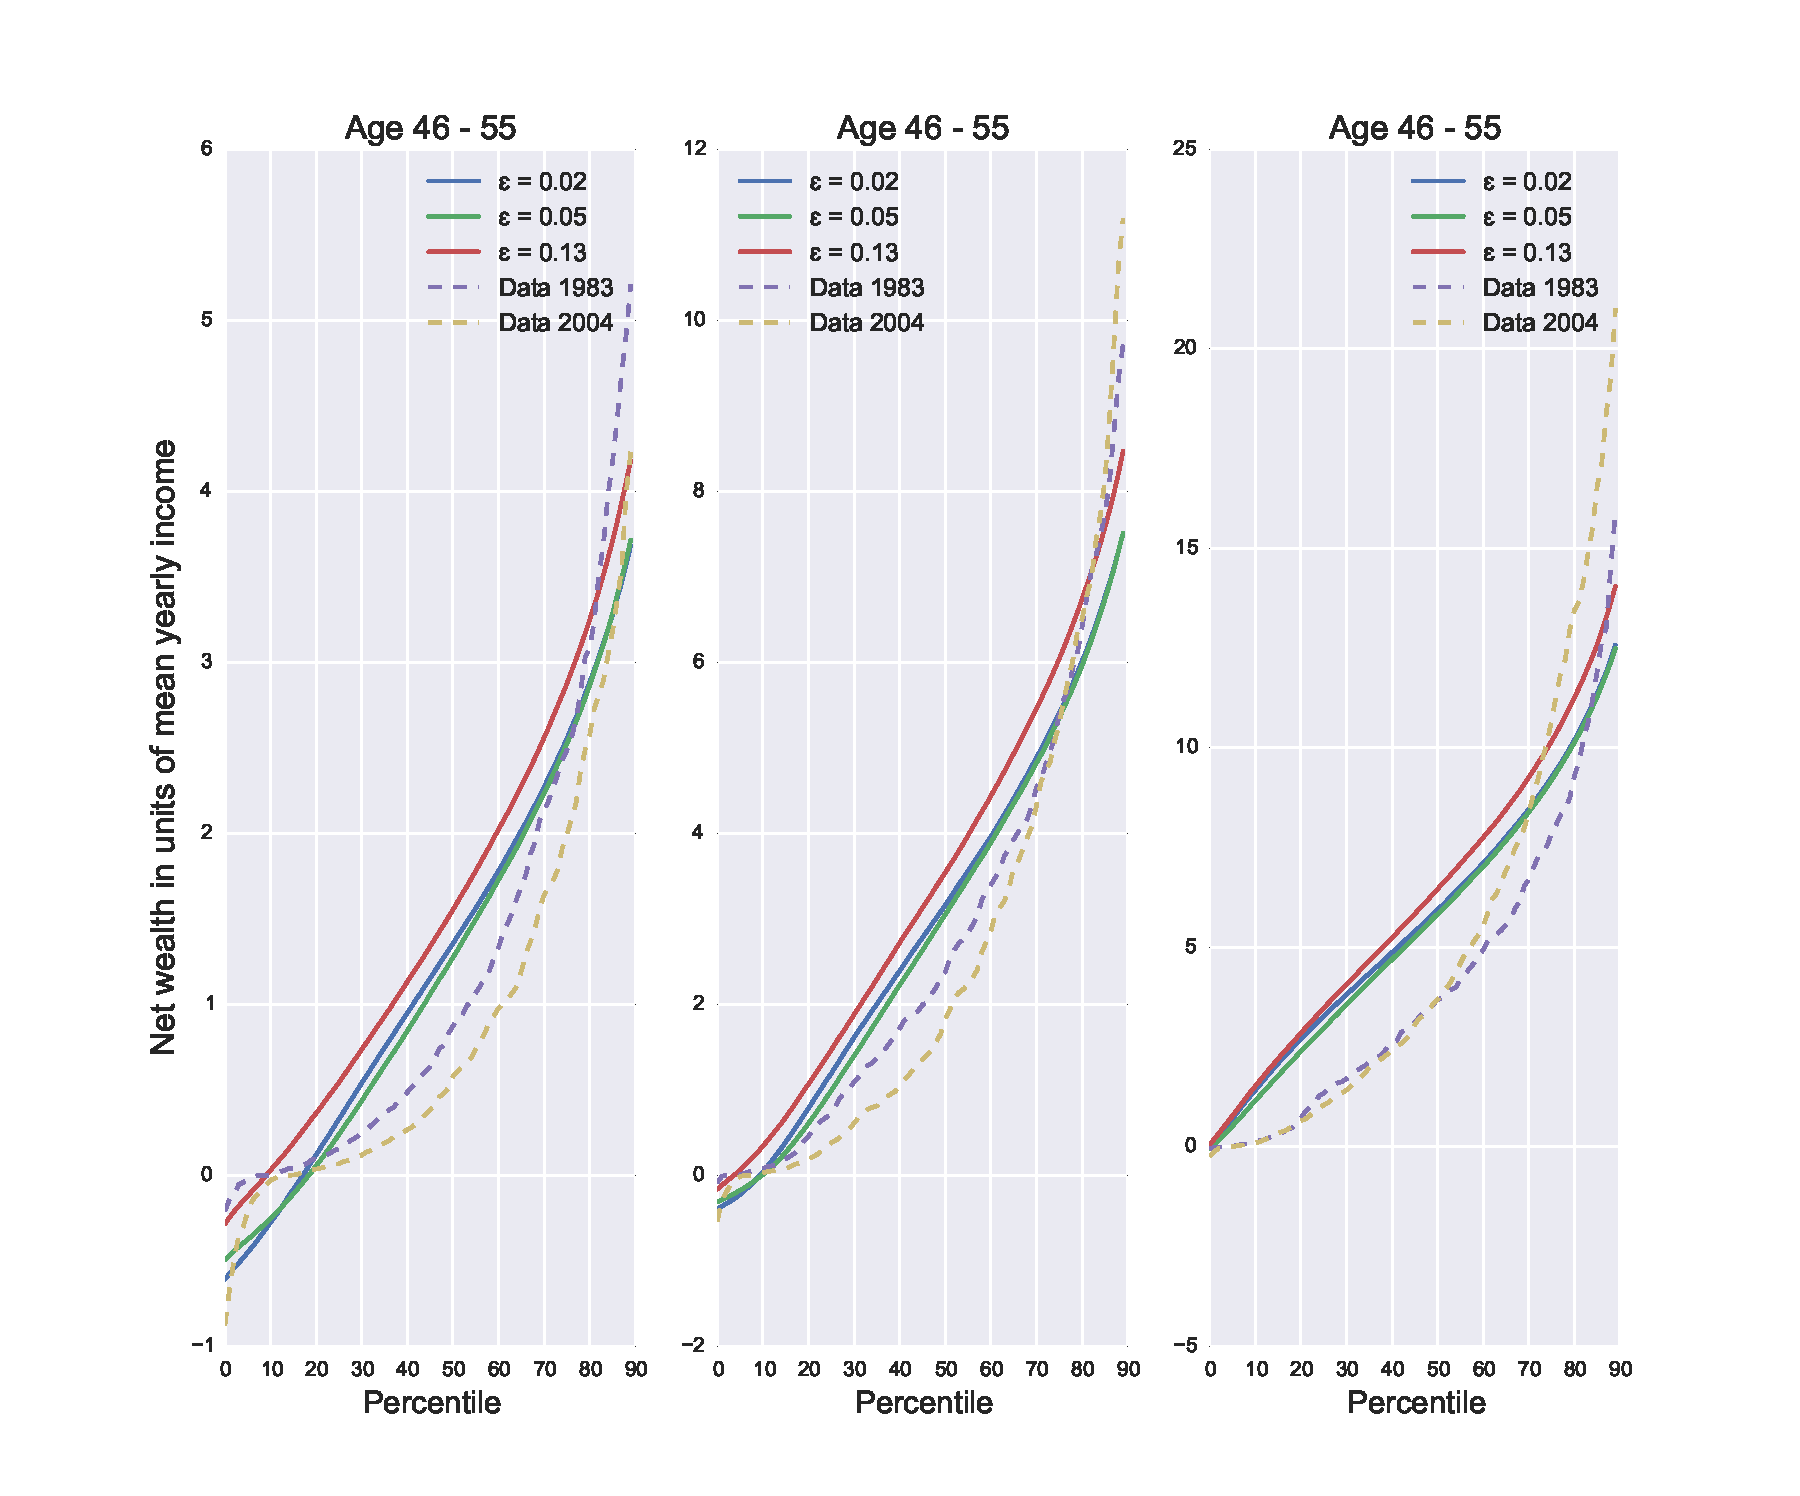
\includegraphics[width=\columnwidth]{comp_stat_eps_agedetail}
\caption{Comparative statics for variance of transitory shocks, by age group}
\label{fig:comp_stat_eps_agedetail}
\end{figure}

\begin{figure}
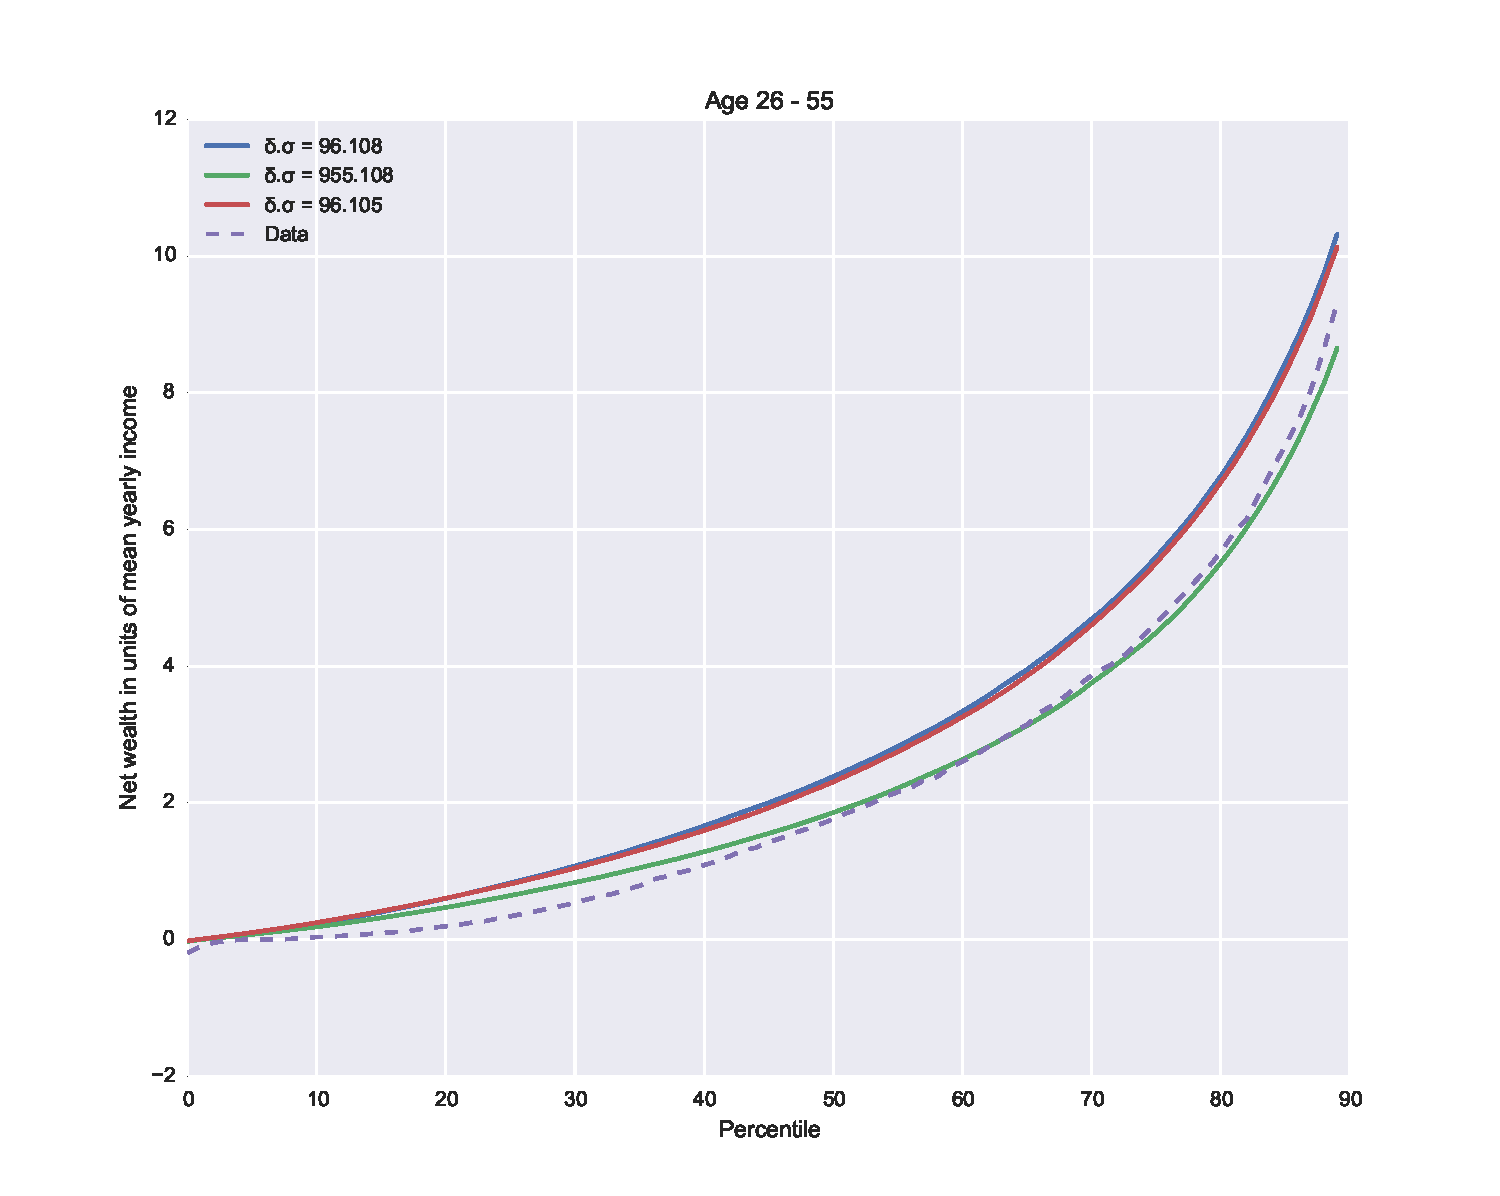
\includegraphics[width=\columnwidth]{winfriedcompare}
\caption{Model fit when income is an RIP process with $\rho=0.95$ and $\sigma^2_{\eta}=0.5$}
\label{fig:winfriedcompare}
\end{figure}

\begin{figure}
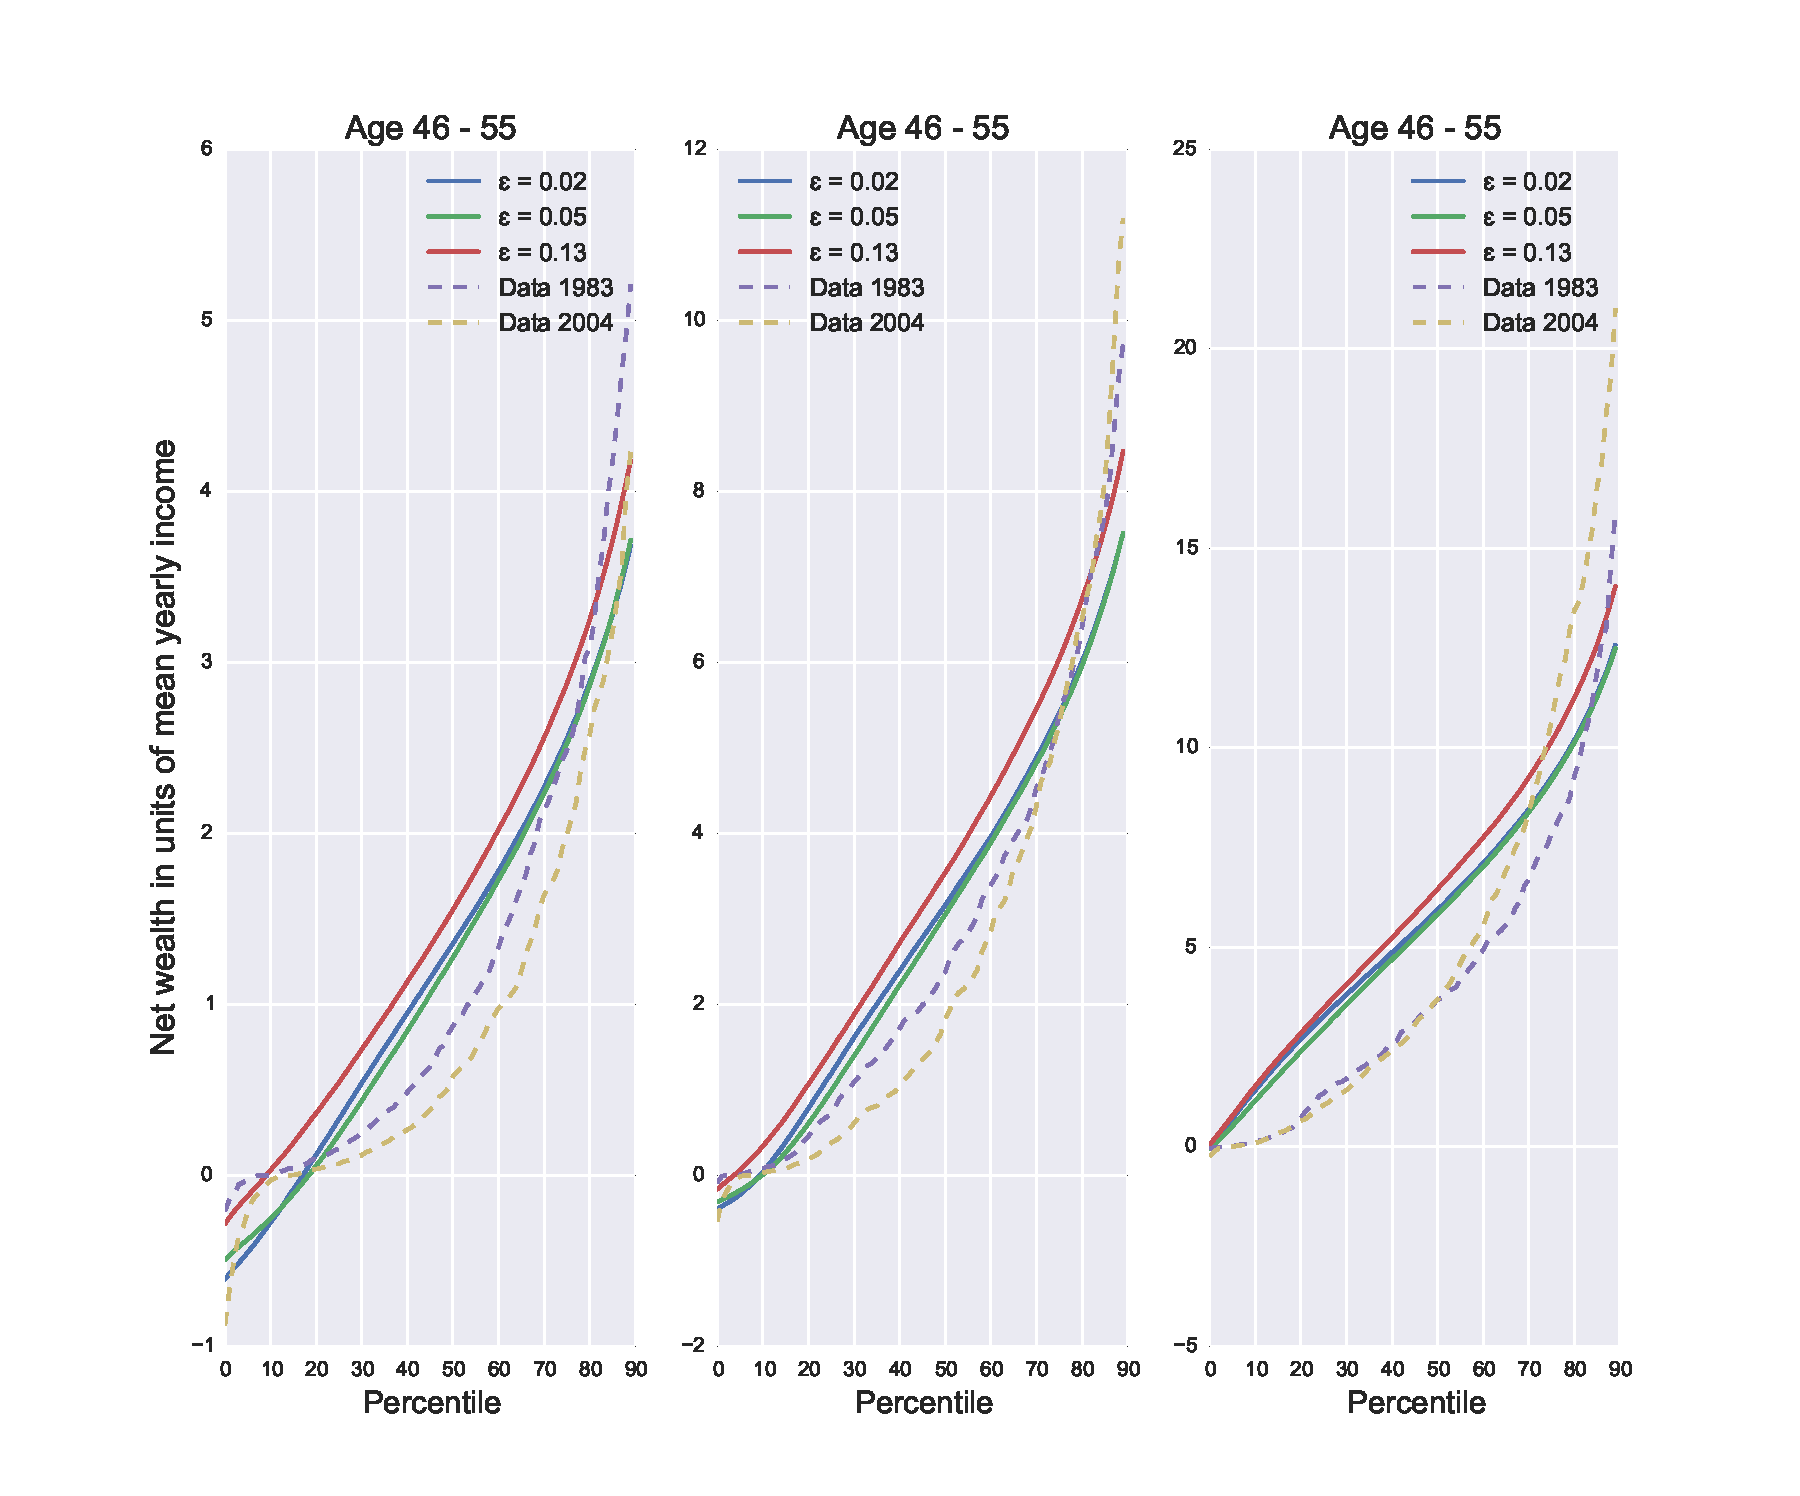
\includegraphics[width=\columnwidth]{comp_stat_eps_agedetail}
\caption{Model fit when income is an RIP process with $\rho=0.95$ and $\sigma^2_{\eta}=0.5$, by age groups}
\label{fig:winfriedcompare_agedetail}
\end{figure}

\begin{figure}
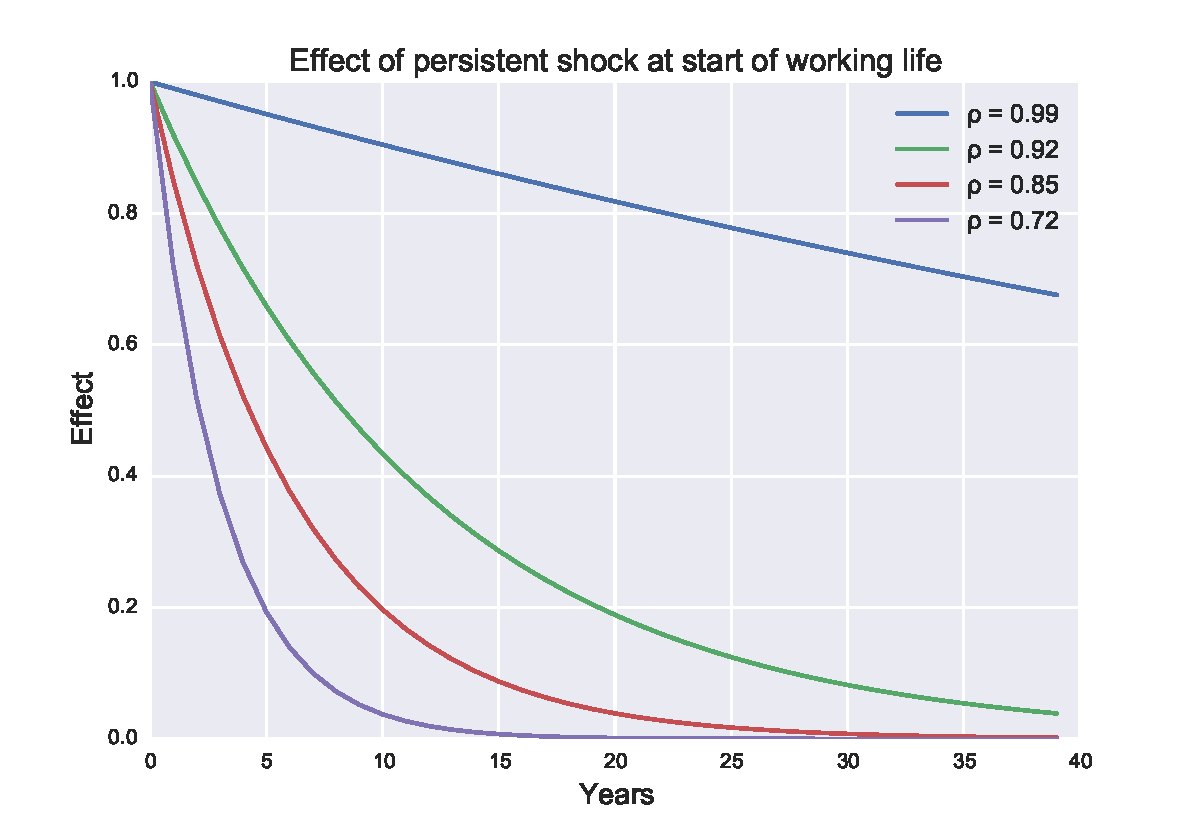
\includegraphics[width=\columnwidth]{effect_rho}
\caption{Effects of lowering $\rho$ on half life of persistent shocks}
\label{fig:effect_rho}
\end{figure}

\chapter{The competitive effects of trade liberalisation in North America: An empirical application of the Melitz and Ottaviano Model} \markboth{\MakeUppercase{\thechapter. TRADE AND PRODUCTIVITY}}{TRADE AND PRODUCTIVITY} 
\section{Introduction}
The economic benefits of free trade are arguably one of the most uncontroversial results of economic research, both theoretically and empirically. However, to this date, free trade is by no means uncontroversial in the public sphere, as is evidenced by the fierce opposition that the proposed transatlantic free trade agreement between the US and Europe is facing. Hence, international trade has remained an active field in economic research, a field which has seen major advancements in the past two decades in incorporating firm-level heterogeneity coupled with consumer love of variety into trade models that can account for the firm-level responses to increasing trade openness and the large share of intra-industry trade in the international flow of goods and services \footnote{A comprehensive survey of trade models with love of variety preferences and firm-level heterogeneity can be found in \citet*{MelitzTrefler2012}.}. This new vintage of trade models predicts additional welfare gains from trade stemming from reallocations of production to more productive firms (as in \citealp{Melitz2003}) or increases in firms' efforts to innovate (as in \citealp{GrossmanHelpman1990}). To some extent, these new models of trade also help reconcile the unambiguously positive stance of economic researchers on trade liberalization with the public opposition to it -- models taking into account explicitly the heterogeneity across agents of firms within a country show that while on aggregate there are significant efficiency gains from free trade, there are also firms and workers who will lose out individually, and can only benefit from a trade liberalization if either the aggregate gains are redistributed in some way to ensure a Pareto improving allocation, or if they can benefit from the reallocation of production to more productive firms by switching to those firms. \citet{DixCarneiro2014} builds a structural model of the Brazilian labor market to estimate the labor market effects of trade liberalization and finds that, depending on the assumptions about capital mobility, the reallocation of workers across sectors can take up to 30 years. \\
While these new models of international trade are well grounded in empirical evidence coming from micro data, there are surprisingly few tests of the model predictions for aggregate variables which are decisive for the predicted welfare gains from trade. Recently, \citet{Arkolakisetal2012a,Arkolakisetal2012b} call into question the importance of firm-level heterogeneity by showing that in a lass class of trade models, the additional welfare gains are fairly small and actually even smaller if consumers don't have CES utility. The response of \citet{MelitzRedding2013} shows that there is still considerable disagreement over how to theoretically evaluate the additional welfare gains from firm selection, and \citet{CostinotRodriguez2014} review the effects of trade liberalizations in a wider class of new trade models to highlight the importance of the market structure under consideration -- depending on whether a one- or multi-sector model is used and the degree of competition assumed, gains from trade are estimated to range from 4\% to 40\% of non-free-trade welfare. These facts m motivate us to test the Melitz-Ottaviano model directly in aggregate data on prices, markups and productivity. To do so, we estimate the effects of trade liberalization on the competitive environment in manufacturing markets of the member countries of the North American Free Trade Agreement (NAFTA). We employ an estimation procedure based on the \citet{MelitzOttaviano2008} model introduced by \citet{Chen2009}, which to our knowledge is the only empirical application of a model with firm-level heterogeneity on aggregate data. \citet{Chen2009} derive estimable regression equations from the model's equilibrium conditions that allow us to test the effects of trade openness on relative price levels, markups and labor productivities of two trading partners. It is further possible to differentiate between the effects of trade in the short run, which, in the model, refers to an economy without relocation decisions for firms, and in the long run, when firms are free to choose their home market for production. However, as the underlying model is static, no direct results on the time path of the impact of trade liberalization can be obtained. We try to address this issue by dividing our sample in ways that make it more amenable to a model-based estimation. Contrary to \citet{Chen2009}, we directly observe tariff rates between the three countries in our sample and hence use those as a direct measure of trade openness. Additionally, we test for the effects of third-country trade openness on the relative performance of two countries that are linked through trade, predictions for which can be derived from the multi-country version of the Melitz and Ottaviano model. Our dataset comprises of nine manufacturing sectors in Canada, Mexico and the US, covering the time period from the introduction of NAFTA in 1994 up to 2006, which gives us reason to believe that we are able to capture the long run effects of policy changes even in industries with low firm churning rates. \\
Our findings support the main model predictions, with tariff barriers stifling domestic competition, leading to higher producer prices and markups as well as lower productivity. In the immediate years after the free-trade agreement when tariff barriers are reduced, relative prices and markups decrease as relative productivity increases, thus giving rise to competitive effects. The results in the long-run, however, are not as clear cut, with some effects reversing as predicted by the model while some effects persist. This is also confirmed by directly looking at the reaction of industries with different entry barriers to changes in trade openness. \\
\vspace{0.5cm} \\
The paper is organized as follows: Section \ref{sec:lit} gives a survey of the previous literature assessing the effects of trade liberalizations in general and of NAFTA specifically. Section \ref{sec:mo} briefly summarizes the Melitz and Ottaviano (2008) model, derives the most important equilibrium conditions and explains the estimation strategy used in \citet{Chen2009}. Section \ref{sec:app} then presents our application of the model by giving an overview of the data used and our estimation procedure. The results of our regressions and possible shortcomings as well as extensions of our approach are discussed in Section \ref{sec:disc4}; Section \ref{sec:conc} concludes.

\newpage

%%%%%%%%%%%%%%%%%%%%%%%%%%%%%%%%%%%%%%%%%%%%%%%%%%%%%%%%%

\section{Related Literature}\label{sec:lit}

As free trade has been an active topic in economic research since the times of Ricardo, the literature on the welfare gains from trade is immense. Of particular interest to us of course are papers that investigate the economic effects of NAFTA directly, as well as papers that form the theoretical foundation for our estimation strategy.

The effects of free trade in North America have been scrutinized in a large number of papers over the past two decades, starting with work on the predecessor to NAFTA, the 1987 Canada and US free trade agreement (CUSFTA). \citet{Head1999} document rationalization effects in Canadian plants as a reaction to decreases in Canadian import duties. \citet{Trefler2004}, focusing on the CUSFTA, uses a reduced form econometric approach to find large improvements in labour productivity and decreases in employment after the implementation of CUSFTA, coupled with slightly lower import prices and larger volumes of trade. \citet*{Fukao2003} derive regression equations from a partial equilibrium model with imperfect competition to estimate the extent to which NAFTA was trade diverting rather than creating and find responses that vary by industry. \citet{Romalis2007} examines both CUSFTA and NAFTA with a strategy based on estimating demand and supply elasticities and finds a large effect of NAFTA on trade volumes, with only minor price changes and, subsequently, only small changes in welfare. \citet{Calderon-Madrid2007} use plant-level panel data from Mexico to show that while productivity increases followed the tariff reductions, the responses of plant-level productivity are very unevenly distributed, with larger plants benefiting disproportionately from productivity increases. The \citet{Melitz2003} model that is at the heart of our analysis is also put to a test with US manufacturing data by \citet*{Bernard2006a}, who use plant-level data to estimate the effects of changes in the costs of trade, as measured by tariff rates and transportation cost, on productivity growth and firm entry and exit. Their findings confirm the micro-level implications derived from the assumptions on the productivity distribution in \citet{Melitz2003}, which we will highlight in the following section. Other papers have used the structure provided by the \citet{MelitzOttaviano2008} model to assess the effects of trade liberalization in other parts of the world: \citet{Bellone2008} use price-cost margins of French manufacturing firms to test the models predictions on the effects of market size, import penetration and exporting status on markups and productivity and confirm that all predictions hold. \citet{Corcos2011} estimate structural parameters in order to simulate counterfactual scenarios by changing the costs of trade between countries. Their exercise shows that the firm selection mechanism is crucial for the magnitude of the welfare gains from trade and the potential gains for a country depend on country size as well as remoteness. The paper that is closest to our own work is \citet{Chen2009}, who use the equilibrium expressions for prices, markups and productivity from the Melitz-Ottaviano model to estimate the effects of trade liberalization using a dataset that includes data on 10 manufacturing sectors in seven European countries for the period 1989-1999 with country-pair regressions. There results suggest that trade openness leads to an increase in competitiveness in the short-run with diminishing and at times reversed effects in the long-run, as predicted by the model. 

%%%%%%%%%%%%%%%%%%%%%%%%%%%%%%%%%%%%%%%%%%%%%%%%%%%%%%%%%

\section{Model and Estimation Equations}\label{sec:mo}

The \citet{MelitzOttaviano2008} model is a synthesis of the contributions of \citet{Melitz2003}, who introduces firm heterogeneity through random draws of a cost parameter for firms entering the market, and \citet{Ottaviano2002}, who develop a model with endogenous markups arising from a linear consumer demand system with horizontal product differentiation. The model yields equilibrium conditions that determine a cost cut-off level, i.e. a level of productivity below which firms are not able to compete in the marketplace. This cut-off level uniquely determines all relevant aggregate variables in the model, namely the distribution of prices, markups and productivity. Importantly, the equilibrium conditions of the model economy are different depending on whether firm entry is allowed or not. Without firm entry, the model captures a short-run equilibrium, with the cost cutoffs in two markets given by:
\begin{align}
N = \bar{N} \left( \frac{c_D}{c_M} \right)^k + \bar{N}^* \frac{1}{\tau^k}\left( \frac{c_D}{c_M^*} \right)^k \label{eq:m-o-supply-n} \\
N^* = \bar{N}^* \left( \frac{c_D^*}{c_M^*} \right)^k + \bar{N} \frac{1}{\left( \tau^* \right)^k}\left( \frac{c_D^*}{c_M} \right)^k \label{eq:m-o-supply-n*}
\end{align}
Here, a star denotes the foreign market, $\bar{N}$ is the fixed number of incumbents in a market and $N$ is the number of firms that are producing. $c_M$ is the upper bound of the distribution of cost draws, $c_D$ is the cut-off level, i.e. the highest cost draw that allows a firm to earn non-negative profits. $\tau>1$ is the iceberg cost of trade faced by foreign companies exporting to the domestic market and can be interpreted as a measure of trade costs, tariffs and other impediments to trade. \\
The long-run equilibrium of the economy allows for firm entry into a market, so that the number of firms in a market is now endogenously determined by a zero profit condition for entrants that balances a fixed cost of entry with the expected profits when drawing a cost level from the (known) cost distribution of a country. The equilibrium conditions pinning down the cost cut-off are
\begin{align}
c_D = \left[ \frac{\phi c_M^k}{L} \frac{1-(\tau^*)^{-k}}{1-(\tau\tau^{*})^{-k}} \right]^{\frac{1}{k+2}} \\
c_D^* = \left[ \frac{\phi c_M^k}{L^*} \frac{1-\tau^{-k}}{1-(\tau\tau^{*})^{-k}} \right]^{\frac{1}{k+2}},
\end{align}
where $L$ is the size of the domestic market. Since all aggregate variables in the Melitz and Ottaviano model are linear functions of the cost cut-off, equations describing the relative price, markup and productivity levels in two countries connected by trade can easily be found by simply dividing the expressions for $c_D$ by those for $c_D^*$. This gives, for the price level in the short run:
\begin{align}
\left( \frac{\bar{p}}{\bar{p}^*} \right)^k = \left( \frac{c_D}{c_D^*} \right)^k = \left(\frac{c_M}{c_M^*} \right)^k \frac{\bar{N}^*}{\bar{N}} \frac{N}{N^*} \frac{1 + \frac{\bar{N}}{\bar{N}^*} \frac{1}{(\tau^*)^k} \left( \frac{c_M^*}{c_M} \right)^k}{1 + \frac{\bar{N}^*}{\bar{N}} \frac{1}{\tau^k} \left( \frac{c_M}{c_M^*} \right)^k} \label{eq:mo-relprice-sr}
\end{align}
and in the long run: 
\begin{align}
\left( \frac{\bar{p}}{\bar{p}^*} \right)^{(k+2)} = \left( \frac{c_D}{c_D^*} \right)^{(k+2)} = \left( \frac{c_M}{c_M^*} \right)^k \frac{L^*}{L} \frac{1-\frac{1}{\tau^k}}{1 - \frac{1}{(\tau^*)^k}} \label{eq:mo-relprice-lr}
\end{align}
These two equations capture one of the central predictions of the Melitz and Ottaviano model: asymmetrical trade liberalizations will have opposing effects on competitiveness in the short and the long run. By equation (\ref{eq:mo-relprice-sr}), lowering trade barriers induces a fall in the cost cutoff, and hence decreases in prices and markups and increases in productivity. In the long run, however, the effects are reversed, as an increase in trade costs induces firms to choose the relatively more protected market for production, thereby increasing competition in markets that are shielded from foreign firms. \\
\citet{Chen2009} show that it is possible to substitute out the trade cost term with an openness term that is derived from a measure of foreign firms market share in the domestic market. However, since we are interested in the effect of tariff rates on competitiveness, we use tariff data directly as a proxy for $\tau$. This strategy should pick up the effects of tariff rates in our estimation if other determinants of trade openness (e.g. oil prices \citep{Kilian2009}, credit conditions \citep{Chor2012}, shared culture and language between countries) do not vary systematically across industries. However, as a first step, we will replicate their analysis exactly in our data set (albeit with different instruments for openness), which requires us to make the same substitution, which is:
\begin{equation}
\frac{1}{\tau^k} \left( \frac{c_M}{c_M^*} \right)^k = \frac{\theta}{1-\theta} 
\end{equation}

Similarly, an expression for the average markup can be derived. The determination of the average markup is equivalent to the one for average prices so expressions for the short-- and long--run impacts of openness on markups can readily be derived. Somewhat more problematic is the index for productivity, as the model requires knowledge of a firm's unit costs $c$, which are not observable. Chen et al. work around this issue by assuming away differences in capital costs, so that average industry productivity can be approximated by the ratio of nominal wages to labour productivity: $\bar{c} = \frac{w}{z}$. If it is additionally assumed that unit labour costs only depend on nominal wages, the ratio of domestic to foreign labour productivity can be written as:
\begin{equation}\label{eq:chen-lab-prod}
\frac{z}{z^*} = \frac{w}{w^*} \frac{\bar{c}^*}{\bar{c}}
\end{equation}
If the least competitive firm in an industry with a productivity draw at the upper bound of the distribution $c_M$ has labour productivity $z_M$ and labour is perfectly mobile between firms, equation (\ref{eq:chen-lab-prod}) implies $\frac{z}{z^*} = \frac{w}{w^*} \frac{c_M^*}{c_M}$. This relationship can then be used in an analogous fashion as before to construct an expression relating openness to productivity. In the short run, equation (\ref{eq:chen-lab-prod}) can be amended to yield:
\begin{equation}\label{eq:chen-prod-sr}
\left( \frac{z}{z^*} \right)^k = \left( \frac{z_M}{z_M^*} \right)^k \frac{(\bar{N}/N)}{(\bar{N}^*/N^*)} \frac{1+ \frac{\bar{N}*}{\bar{N}} \frac{\theta}{1-\theta}}{1+ \frac{\bar{N}}{\bar{N}^*} \frac{\theta^*}{1-\theta^*}} 
\end{equation}
Higher values of $\theta$ thus lead to higher productivity (conditional on $\bar{N}/N$), as they force lower productivity firms to shut down production. For the long run, equation (\ref{eq:mo-relprice-sr}) combined with the expression for labour productivity gives:
\begin{equation}\label{eq:chen-prod-lr}
\left( \frac{z}{z*} \right)^{k+2} = \left( \frac{w}{w^*} \right)^2 \frac{L}{L^*} \left( \frac{z_M}{z_M^*} \right)^k \frac{1-\frac{\theta}{1-\theta}}{1-\frac{\theta^*}{1-\theta^*}}
\end{equation} 
Larger markets exhibit higher labour productivity, while the effects of $\theta$ and $\theta^*$ are the opposite of those in the short--run.

%%%%%%%%%%%%%%%%%%%%%%%%%%%%%%%%%%%%%%%%%%%%%%%%%%%%%%%%%

\subsection{The Role of Market Entry}
Following the arguments in \citet{Trefler2004}, we want to exploit the nature of NAFTA being close to a natural experiment and hence try to identify the effect of the policy measures (i.e. the changes in tariff rates) separately from the effects of trade openness in general. There is evidence that trade openness -- measured by the import penetration of a certain country or industry, as in \citet{Chen2009} -- is affected by a number of external forces, including oil prices \citep{Kilian2009}, credit conditions \citep{Chor2012}, shared culture and language between countries and many more. Therefore, we deconstruct the iceberg costs of trade into two parts: $\tau^{lh}=\frac{Tr^{lh}}{\theta^{lh}}$, where $Tr^{lh}>1$ is the tariff rate for trade between countries $l$ and $h$ and $\theta^{lh}>1$ captures the additional costs of trade imposed by the aforementioned factors. Then, the import penetration can be viewed as a measure of $\theta^{lh}$, as in Chen et al. (2009), while a carefully constructed tariff measure can directly account for the effect of NAFTA-mandated changes in the trade environment. Obviously, the import penetration in a sector depends on the tariff measure as well, so an instrumental variable approach has to be taken in order to identify this effect. We defer the discussion of the construction of the tariff measure and the choice of instruments to the following chapter. Prior work of \citet{Bernard2006} suggests that tariff rates throughout the 1980s, at an average level between four and five percent, accounted for about the same fraction of trade costs as costs directly attached to shipping the good, i.e. freight and insurance, so we expect them to have a sizeable impact on trade flows between countries and hence the competitive environment. \vspace{0.5cm} \\

As we have seen in the exposition of the Melitz and Ottaviano model above, there is one crucial caveat in taking the model to the data: due to the static nature of the model, the comparative static results just compare one steady state with another, while being silent about the transitional dynamics. The estimation strategy of \citet{Chen2009} tries to account for this by estimating an error correction model to identify the long-run separately from the short-run, but their results -- just as ours -- are mixed for the long run and it cannot be ruled out that this is due to the estimation procedure. Therefore, we try to address this issue in a more direct way: as short- and long-run in the model differ only in the possibility of firm entry, we separate industries into those with a fixed number of firms and those with low entry barriers. This distinction then gives us industries that represent the short- and long-run and we can directly investigate whether the coefficients on the relevant variables differ significantly\footnote{We were inspired to do so by \citet{Head1999} who use the classification to test competing theories of trade that rely on different market structures.}. This approach, however, leads to two issues that need to be addressed before implementation. First, it is not \textit{a priori} obvious how to measure the entry conditions in an industry; while the theoretical model uses the number of firms, this could in practice either refer to firms or to establishments (i.e. different production sites run by the same parent company), or even to employees, as firms in the model use unit labour input. Second, there is no reason to believe that different measures of entry and exit dynamics are exogenous with respect to trade openness -- indeed in the model trade openness is a key factor in the entry decision of firms, but in the real world there might be various other factors that might lead to industries being asymmetrically affected by a change in trade costs, hence biasing our results. To tackle both these issues, we aim to construct a robust measure of industry dynamics by aggregating multiple studies that examine firm and employment turnover in Canada, Mexico and the United States as well as Europe over different time periods. With this, we hope to identify those industries that are either very dynamic or very static over a broad set of different measures, regions and time periods. Table \ref{tb:market_lit} gives an overview of the studies used and a glance at their respective results, showing considerable variation in the dynamics of entry and job creation in different manufacturing sectors.
 
\begin{center}
\begin{table}
\begin{tabular}{|p{2.8cm}|p{4cm}|p{4cm}|p{4cm}|}
\hline
\textbf{Study}  &  \textbf{Subject}  &  \textbf{Highest Turnover}  & \textbf{Lowest Turnover} \\
\hline 
\hline
\citet{Dunne1988} & Entry Rates (4-yearly) \newline U.S. \newline 63-82    & Instruments (60.3) \newline Lumber (49.70) \newline Printing (49.0)  & Leather (29.4) \newline  Food Processing (23.9) \newline Tobacco (20.5) \\  
\hline
Samianego (2008)   & Entry Rates (yearly)  \newline Europe \newline 97-04  & Paper, printing, software (15.6) \newline Textiles (11.9) \newline Petroleum and Coal (11.9) & Chemicals (9.5) \newline Plastics (9.4) \newline Food Products (9.1) \\
\hline 
\citet{Brown2004}  & Employment renewal    \newline Canada \newline 73-96  & Plastic (79.5) \newline Furniture (79.4) \newline Fabricated Metals (77.2) & Primary Metals (33.6) \newline Paper (32.4) \newline Tobacco (4.2) \\
\hline
\citet{Foster2006} & Job creation (yearly) \newline U.S. \newline 72-98     & Lumber (11.8) \newline Apparel (11.2) \newline Miscellaneous (11.0) & Paper (5.9) \newline Petroleum (5.9) \newline Tobacco (5.1) \\
\hline
\citet{Baldwin1994} & Job turnover (yearly) \newline Canada \newline 73-86 & Furniture (26.5) \newline Machinery (26.3) \newline Lumber (25.7) & Petroleum (14.1) \newline Primary Metals (13.5) \newline Paper (10.7)  \\
\hline
\citet{Baldwin1994} & Job turnover (yearly) \newline U.S. \newline 73-86 & Lumber (27.2) \newline Apparel (25.5) \newline Leather (22.5) & Petroleum (14.6) \newline Chemicals (14.0) \newline Paper (13.3) \\
\hline   
\end{tabular}\caption{Market Structure measures used, numbers in percent}\label{tb:market_lit}
\end{table} 
\end{center}

In order to aggregate the different studies, we compute percentile-based rankings of the industries for each study (to account for the different number of industries across studies) and then average the percentiles across studies. Based on these average percentiles, we can then split the sample according to the short- and long-run distinction made in the model: those industries above the 60th percentile are taken to represent the dynamic, "free entry" sample and thus the long run, while those industries below the 40th percentile are taken to represent the short run. This procedure leads us to split the sample three-ways: Food, Beverages and Tobacco, Textiles as well as Chemicals, Fuels, Plastics, Rubber fall into the long run category, Machinery and Transportation Equipment, Manufacturing not else classified and Wood and Cork make up the short run category. The three remaining industries (Paper and Printing, Basic and Manufactured Metal Products and Other Non-Metallic Mineral Products) are too close to the median to be classified either way and are thus dropped from the sample\footnote{Due to different classification systems, the aggregation of studies was not always exact and some industry groups are quite heterogeneous when sub-industries are considered. For further details on the aggregation see Appendix B}. \\
A little thought experiment may clarify the role that market entry effects play in muddling the distinction between short-- and long--run equilibria. The Melitz and Ottaviano (2008) model yields opposing predictions on the effects of trade liberalization on country-level economic variables such as prices, productivity and mark-ups. The reason for the differences, as we have seen, lies in the assumptions on market structure: there are two different equilibria depending on whether entry into a market is allowed. We repeat them here for convenience:
\begin{align*}
c_D^k &= c_M^k \frac{\bar{N}^*}{N^*} \left( 1+ \frac{\bar{N}}{\bar{N}^*} \frac{\theta^*}{1-\theta^*} \right) \\
c_D^{k+2} &= \frac{\phi c_M^k}{\Upsilon L} \left(1- \frac{\theta^*}{1-\theta^*} \right)
\end{align*}
In model terms, only one of these two equations holds at any given time, and it is posited that the first equation captures the short run effects of trade liberalization, while in the long run firms are allowed to enter the markets and the effects of trade barriers are determined by the second equation. No further assumptions on the nature of the firm's entry decisions or capital adjustment costs are made that could help separate short- from long run. However, in reality, it seems to be more natural to assume that there is a gradual evolution from one equilibrium to the other, and this view is borne out by data on firm entry and exits showing that in a given year, only between five and ten percent of firms in a given industry are new entrants, while over longer horizons this figure goes up to 80 percent. Hence, it seems to be reasonable to model the transition from the short- to the long run equilibrium by introducing a parameter $\alpha$ that governs the fraction of firms entering an industry. The effects of this parameter are most clear on the productivity side, given that firms cannot change their productivity level, the new productivity distribution will be a weighted average of new entrants' and existing firms' productivity. As the examples in Chen et al. are formulated with respect to relative prices, and we are using their notation, we will discuss the effects of limited firm entry in the price level case as well. The argument carries through if one is ready to assume a nominal rigidity that prevents incumbents from re-optimizing their prices, similar to the assumptions made in New Keynesian monetary models. Similar to the productivity level, the price level is then a weighted average of new and old prices (for simplicity, here we abstract from substitution effects induced by the new relative prices of new and old producers):
\begin{align*}
\bar{p} &=\alpha \bar{p}^{LR} + (1-\alpha) \bar{p}^{SR} \\
				&=\alpha c_D^{LR} + (1-\alpha) c_D^{SR} \\
        &=\alpha \left( \frac{\phi c_M^k}{\Upsilon L} \left(1- \frac{\theta^*}{1-\theta^*}  \right) \right)^{\frac{1}{k+2}} + (1-\alpha) \left(c_M^k \frac{1}{ \frac{\bar{N}}{N}\left( 1+ \frac{\bar{N}^*}{\bar{N}} \frac{\theta}{1-\theta} \right) } \right)^{\frac{1}{k}}							
\end{align*}
where the second line drops the constant linking price level and cost cut-off for notational simplicity. It can easily be seen that the introduction of the $\alpha$ parameter makes the expression for the price level hugely complicated and eliminates the possibility to cancel out most constant terms by using relative prices as was done in \citet{Chen2009}. Obviously, the above expression is impossible to take to the data in the hope of identifying any of the parameters. \\
Let's consider a simplified version of the above. Assume that relative prices levels in the short- and long run, respectively, are given by:
\begin{align*}
\frac{\bar{p}^{SR}}{\bar{p}^{*SR}} = \left( \frac{c_M}{c_M^*} \right)^k \frac{(\bar{N}^* / N^*)}{(\bar{N} / N)} \frac{\rho^*}{\rho} \\
\frac{\bar{p}^{LR}}{\bar{p}^{*LR}} = \left( \frac{c_M}{c_M^*} \right)^k \frac{L^*}{L} \frac{(1-\rho^*)}{(1-\rho)}
\end{align*}
This is a simplified version of the equilibrium conditions in Chen et al. using the notation of Melitz and Ottaviano in which trade freeness is measured by $\rho \in (0,1)$. It captures the main essence of the model, in the short run relative prices depend on the number of firms and negatively on trade freeness (increasing $\rho$ will decrease $\bar{p}$), while in the long country size matters and prices depend positively on trade freeness (increasing $\rho$ decreases $1-\rho$ and thus increases $\bar{p}$). Now assume further, that price setting decisions and substitution behavior of consumer is such that we can aggregate \textit{relative} price levels in the same way we aggregated individual price levels before. Then:
\begin{align*}
\frac{\bar{p}}{\bar{p}^*} &= \alpha \frac{\bar{p}^{LR}}{\bar{p}^{*LR}} + (1-\alpha) \frac{\bar{p}^{SR}}{\bar{p}^{*SR}} \\
													&= \alpha \left( \left( \frac{c_M}{c_M^*} \right)^k \frac{L^*}{L} \frac{(1-\rho^*)}{(1-\rho)} \right) + (1-\alpha) \left( \left( \frac{c_M}{c_M^*} \right)^k \frac{(\bar{N}^* / N^*)}{(\bar{N} / N)} \frac{\rho^*}{\rho} \right)
\end{align*}
Here, the fundamental identification problem becomes apparent: in the first term on the right hand side of the equation, the effect of $\rho$ on $\bar{p}$ is positive, while in the second term it is negative. However, the size and sign of the composite effect will be governed by $\alpha$, which is unobservable. In order to estimate the effects of trade openness on prices, we have to control for firms entry behavior. While this might well be endogenous to changes in trade policy, it is reasonable to assume that different industries have different entry conditions due to fixed costs inherent in the business model. We can try to exploit this variation in entry conditions by sorting businesses according to the ease of entry; then, ceteris paribus, an industry with lower barriers to entry should exhibit a response to trade liberalization along the lines that the model predicts for the long run equilibrium (as the value of $\alpha$ increases, $\bar{p}$ approaches $\bar{p}^{LR}$), while an industry with high entry barriers subject to the same trade liberalization should see a very different reaction. \\
One way to alleviate this problem is by trying to use information on $\alpha$ in the estimation. Splitting the sample based on our aggregated turnover measures can be seen as a crude approximation to this, as can be the construction of dummy variables for high and low turnover industries. The most direct way, however, would be to use information on industry turnover rates directly. Obviously, this brings back the very same endogeneity problems we described above that were one reason to aggregate the studies in the first place, which makes it important to instrument for entry and exit rates in industries using turnover measurements for different periods than the one considered in the estimation. The variable construction will be explained in more detail in the next section.

\section{Application}\label{sec:app}
Starting from the equations for prices, productivity and markups derived within the Melitz-Ottaviano framework, we can derive estimable log-linearized equations analogous to those in Chen et al. The estimation equation for prices is given by:
\begin{align}
\begin{split}\label{eq:gw-estimation-prices}
\Delta \ln \left( \frac{\bar{p}_{it}}{\bar{p}_{it}^*} \right) = &\beta_0 + \beta_1 \Delta \ln \tau_{it} + \beta_2 \Delta \ln \tau_{it}^* + \beta_3 \Delta \ln D_{it} + \beta_4 \Delta \ln D_{it}^* \\ &+ \gamma \left[ \ln \left( \frac{\bar{p}_{it-1}}{\bar{p}_{it-1}^*} \right) + \delta_0 + \delta_1 \ln L_{t-1} + \delta_2\ln L_{t-1}^* + \delta_3 \ln  \tau_{i,t-1} + \delta_4 \ln  \tau_{i,t-1}^* \right] + \varepsilon_{ijt} 
\end{split}\end{align}
In the above equation, the number of firms serving the domestic market, $N$, has been replaced by the more readily observable number of domestic firms producing for the domestic market, $D$, where $D=N \left( \frac{c_D}{c_M} \right)^k$. The short--run dynamics are estimated in the first part of the equation, with regressors expressed in first differences. The long run is represented by the term in brackets. From the perspective of this model, we would expect $\beta_1>0$, an increase in domestic import tariffs increases relative prices in the short-run, and correspondingly $\beta_2>0$. The model predicts a dampening effect of the number of domestic firms on domestic prices, which should be reflected by $\beta_3<0$, and the opposite for foreign firms, $\beta_4<0$. As we expect the coefficient on the error correction term, $\gamma$, to be negative, a reversal the 

As previously discussed, all aggregate variables (prices, markups, productivity) are ultimately functions of the cost-cutoff level $c_D$, leading to very similar estimation equations for our three dependent variables. The equation markups is:
\begin{align}
\begin{split}\label{eq:gw-estimation-markup}
\Delta \ln \left( \frac{\bar{\mu}_{it}}{\bar{\mu}_{it}^*} \right) = &\beta_0 + \beta_1 \Delta \tau_{it} + \beta_2 \Delta \tau_{it}^* + \beta_3 \Delta \ln \theta_{it} + \beta_4 \Delta \ln \theta_{it}^* + \beta_5 \Delta \ln D_{it} + \beta_6 \Delta \ln D_{it}^*\\ 
&+ \gamma \left[ \ln \left( \frac{\bar{\mu}_{it-1}}{\bar{\mu}_{it-1}^*} \right) + \delta_0 + \delta_1 \ln L_{t-1} + \delta_2\ln L_{t-1}^* + \delta_3  \tau_{i,t-1} + \delta_4  \tau_{i,t-1}^* \right] + \varepsilon_{ijt} 
\end{split}
\end{align}
The effect of tariffs, openness, number of firms and market size on productivity is estimated by:
\begin{align}
\begin{split}\label{eq:gw-estimation-productivity}
\Delta \ln \left( \frac{\bar{z}_{it}}{\bar{z}_{it}^*} \right) =&\beta_0 + \beta_1 \Delta \tau_{it} + \beta_2 \Delta \tau_{it}^*  + \beta_3 \Delta \ln D_{it} + \beta_4 \Delta \ln D_{it}^*\\
&+ \gamma \left[ \ln \left( \frac{z_{it-1}}{z_{it-1}^*} \right) + \delta_0 + \delta_1 \ln L_{t-1} + \delta_2\ln L_{t-1}^* + \delta_3  \tau_{i,t-1} + \delta_4  \tau_{i,t-1}^*  \right. \\ 
&+ \left. \delta_5 \ln w_{i,t-1} +  \delta_6 \ln w_{i,t-1}^* \bigg] \right. + \varepsilon_{ijt} 
\end{split}
\end{align}
where $\delta_7$ and $\delta_8$ capture the effects of changes in nominal wages in the long run. The intercepts $\beta_0$ are introduced to capture differences in country--specific technology as Chen et al. depart from the baseline Melitz-Ottaviano model by allowing for such differences. While in the baseline, these vary by country-pair, we check the robustness of the specification by allowing fixed effects at a sectoral level. 

\subsection{Preferential Trade Liberalization}
The model results and estimation equations presented so far all referred to a 
unilateral trade liberalization in a simplified two-country setup\footnote{Note
 that a bilateral trade liberalization -- changing $\tau$ and
 $\tau^*$ by the same amount -- would not lead to the discussed short- and long 
run changes in cost cutoffs for two countries, but instead to a decline in the cost cutoffs in both countries both in the short and the 
long run.}. While making the exposition clearer and helping to elicit the effects at work in the model, this setup is clearly not an accurate description of the reality of trade relationships in modern industrialized economies. Taking the United States as an example, while the two other countries in our data set, Canada and Mexico, are its largest 
trading partners, they only account for 16.6 and 13.5\% of all US trade by value, 
respectively\footnote{See \href{http://goo.gl/2C0saQ}{Top U.S. Trade Partners, U.S. International Trade Administration}}. 
Even the largest 30 US trading partners only account for about 86\% of US trade, highlighting the fragmented nature of international trade. While the Melitz-Ottaviano model can be extended to an arbitrary number of countries, it is clearly not feasible to assemble a data set on all trade partners of the NAFTA countries. We do however want to recognize the multi-country structure of NAFTA by taking into account third country effects of trade barriers. Here, NAFTA can be interpreted as a preferential liberalization of Mexico \textit{vis-a-vis} the US and Canada, as Mexico had the highest tariff barriers to start off with. In the three country case, we expect the country with the lowest sum of bilateral trade barriers to have the lowest cost cutoff, as it becomes the best export hub. To account for this, we amend equations \ref{eq:gw-estimation-prices}, \ref{eq:gw-estimation-markup} and \ref{eq:gw-estimation-productivity} by including the relevant third country tariffs. The estimation equation for the effects of trade barriers on prices then becomes:

\begin{align}
\begin{split}\label{eq:gw-estimation-prices-third-country}
\Delta \ln \left( \frac{\bar{p}_{it}}{\bar{p}_{it}^*} \right) = 
&\beta_0 + \beta_1 \Delta \ln \tau_{it} + \beta_2 \Delta \ln \tau_{it}^* + \beta_3 \Delta \ln \tau_{it}^{ht} 
+ \beta_4 \Delta \ln \tau_{it}^{th} + \beta_5 \Delta \ln \tau_{it}^{ft} + \beta_6 \Delta \ln \tau_{it}^{th} \\ 
&+ \beta_7 \Delta \ln D_{it} + \beta_8 \Delta \ln D_{it}^* + \beta_9 \Delta \ln D_{it}^t \\ 
&+ \gamma \left[ \ln \left( \frac{\bar{p}_{it-1}}{\bar{p}_{it-1}^*} \right) + \delta_0 + \delta_1 \ln L_{t-1} + \delta_2\ln L_{t-1}^* 
 + \delta_3 \ln L_{t-1}^t+ \delta_4 \ln \tau_{i,t-1} \right. \\ 
&+ \left. \delta_5 \ln  \tau_{i,t-1}^*  + \delta_6 \Delta \ln \tau_{it}^{ht} + \delta_7 \Delta \ln \tau_{it}^{th} 
 + \delta_8 \Delta \ln \tau_{it}^{ft} + \delta_9 \Delta \ln \tau_{it}^{th} \bigg] \right. + \varepsilon_{ijt} 
\end{split}\end{align}
where now $h$ is the domestic economy, $f$ is the foreign economy, and, with a slight abuse of notation, a $t$ superscript denotes the third country for each country pair (e.g. when estimating the Canada-US relationship, $\tau^{th}$ are Mexican tariffs on Canadian goods, while $\tau^{ht}$ are Canadian tariffs on Mexican goods). Both the equations for markups and productivity will be amended accordingly. 

\subsection{Dataset}

The database we utilize covers the period 1994-2006 for NAFTA member countries -- Canada, Mexico, and the US -- and nine manufacturing sectors. For our factory gate price data, we use the producer price index (PPI) as reported by CANSIM, the Banco de Mexico, and the U.S. Bureau of Labor Statistics, respectively. All indices are normalized to equal 100 in 2003. While the majority of the manufacturing data collected is reported at the two-digit level according to ISIC Rev. 3, we aggregate all data according to NACIS in order to keep consistency throughout the analysis (see Table \ref{tb:isic_class} for the manufacturing classification breakdown). While the main part of our analysis rests on data aggregated at the two-digit level, we were also able to assemble a data set at the four-digit level, which we will use to check the robustness of our results. 

The value of markups is not easily observable, and thus we follow the calculation as outlined in the recent literature on industrial organization, and similarly used by \citet{Chen2009}, although with a subtle modification. We compute average markups as the ratio of sectoral turnover relative to total variable costs, which are computed as the sum of intermediate inputs and labor costs as reported by the OECD STAN database.\footnote{In contrast, \citet{Chen2009} calculate average markups as the ratio of turnover relative to the sum of the costs of materials, consumables, and staff costs.} Due to the unavailability of data on sectoral turnover, we use sectoral production as a proxy. While turnover may be slightly higher than production\footnote{Production represents the value of goods produced in a year, whether they are sold or stocked.} in a given year if all of the produced goods are sold along with any stored goods from previous years, according to the OECD these measures will converge in the long term. Fixed costs are excluded from the calculation, as they will cause a negative bias between markups and openness. As the number of foreign firms increases due to a decrease in trade costs, the market share for domestic producers falls; because this will spread fixed costs across a smaller share of production, average total costs will increase contemporaneously \citep{Chen2009}. 

Labor productivity is calculated as the ratio between real value added and total employment. Value added is reported by the OECD STAN database, while employment data is provided by LABORSTA, the statistical department of the International Labor Organization (ILO). 

The main explanatory variable in this analysis is the tariff imposed on foreign products. The simple average for tariffs disaggregated at the two-digit level (ISIC Rev. 2) imposed on the bi-lateral trading partners within NAFTA were taken from the World Integrated Trade Solution (WITS), which is a resource developed by the World Bank. The changes in import tariffs across all industries for each country-pair are illustrated in Figures \ref{fig:can_mex} -- \ref{fig:usa_mex}, including the maximum and minimum tariff for each year. The tariffs imposed by the U.S. on Canadian and Mexican goods, and those imposed by Canada on Mexican and U.S. goods approached zero by 1999--2000, while the Mexican imposed tariffs fluctuated drastically throughout the time period, with some tariffs reaching 30\%. The average, maximum, and minimum tariffs by country and sector are also detailed in Table \ref{tab:sumstats}, as well as the other main variables in this analysis.

To construct the openness variable, we calculate the ratio of imports relative to the sum of imports and domestic production, as in \citet{Chen2009}. The bilateral trade data for each country-pair comes from the OECD STAN database and measured in current USD. Domestic production is calculated as the difference between total sectoral output and exports. The sectoral output data are also taken from the OECD STAN database (measured in current units of national currency) and converted to current USD using the OECD-reported exchange rates. In order to check the reliability of our measure of openness, we also use the UPenn openness index. 

As discussed in the previous section, for all of the log-linearized equations, we replace the number of firms serving the domestic market, $N$, with the number of domestic firms producing for the domestic market, $D$. Unfortunately, this data is not available for all three countries during the specified time period, and thus we utilize the number of establishments, which will always be higher than the firm count as each firm may have multiple establishments. As long as the average number of establishments per firm remains constant, this should not present a problem, as our model is estimated in first differences. It is however not obvious that this relationship will remain constant in response to a trade liberalization. In fact, the main channel through which welfare gains arise in the model is the reallocation of production from unproductive to more productive firms, with less productive firms exiting the market and more productive firms expanding. If this displacement happens through larger firms taking over establishments of less productive ones, we would expect the number of establishments to stay constant, while the number of domestic producers falls (i.e. the number of establishments per firm increases). If on the other hand larger firms are simply able to expand production in existing establishments, this effect would be absent.  

The control variables used in the regressions include nominal wages and size of the economy, both of which are provided by LABORSTA. Wages are disaggregated according to ISIC Rev. 3 and reported in national currency units per hour for all wage earners (as before, we convert all data into ISIC Rev. 2 and current USD). For the size of the economy $L$, we utilize the total economically active population for manufacturing. Moreover, there are missing values for the US and Mexico\footnote{We use interpolated data for the years 1999, 2001, and 2003 for the US, and 1992, 1994, 1996, 1998, 2001-2003 for Mexico.} and thus we use interpolated data for these years.

\subsection{Estimation}
As outlined at the beginning of Section \ref{sec:app}, we follow the estimation strategy of Chen et al. (2009); however, while they use changes in domestic and foreign import penetration in sector $i$ at time $t$ as the main explanatory variables for changes in price, markups, and labor productivity, we use this as a control variable and instead rely on the domestic tariff rate ($\tau$) imposed on foreign goods imported from the trading partner and the foreign tariff rate ($\tau^*$) imposed on domestic goods exported to the trading partner as the main explanatory variables. To test the competitive effects of trade liberalization, we use the difference in differences approach with fixed--effects on the country--pair, industry, and year. In the short run we use the log first-difference in the explanatory and dependent variables, whereas we use a lag operator on the explanatory variables and an error correction term to estimate the dynamics in the long run. Moreover, because our variables are stationary in a unit root sense and serially correlated, we utilize a panel-specific AR(1) autocorrelation structure and perform our regressions using a Generalized Least Squares estimation strategy. 

Table \ref{tb:comp_stats} outlines the comparative statics for the theoretical model, with subscript $sr$ denoting the "short run" and $lr$ denoting the "long run". Notice that in the long run theory suggests that the pro--competitive effects are reversed and actually take an anti--competitive nature as firms are able to relocate to new markets. Interestingly, as we will exhibit in the following section, our analysis does not provide the same long-run dynamics.

\begin{center}
\begin{table*}[ht] \caption{Comparative Statics -- Model Predictions}\label{tb:comp_stats}
\vspace{0.5cm}
{\small
\hfill{}
\begin{tabular}{|l|c|c|c|c|c|c|}
\hline
\textbf{Regressor}& \multicolumn{6}{|c|}{\textbf{Dependent Variables}}\\
\cline{2-7}
\hline
& $\bar{p}_{sr}$ & $\bar{p}_{lr}$ & $\mu_{sr}$ & $\mu_{lr}$ & $z_{sr}$ & $z_{lr}$ \\ \hline
$\tau$     & +  & -- & +  & -- & -- & + \\ \hline
$\tau^*$   & -- & +  & -- & +  & +  & --\\ \hline
$D$        & -- &    & -- &    & +  &   \\ \hline
$D^*$      & +  &    & +  &    & -- &   \\ \hline
$L$        &    & -- &    & -- &    & + \\ \hline
$L^*$      &    & +  &    & +  &    & --\\
\hline
\end{tabular}}
\hfill{}
\end{table*}
\end{center}


\section{Results \& Discussion}\label{sec:disc4}
Tables \ref{tb:prices_sr}, \ref{tb:markup_sr} and \ref{tb:productivity_sr} present our results on the short-run effects of trade liberalization on prices, markups and productivity, respectively. Column (1) in each table presents the results from our theoretical estimations in equations \ref{eq:gw-estimation-prices}, \ref{eq:gw-estimation-markup}, and \ref{eq:gw-estimation-productivity}, respectively. Beginning with table \ref{tb:prices_sr}, we see that the signs on the tariff measures are as predicted -- a decrease in the domestic tariff will decrease the relative price in the short-run -- but only the foreign tariff measure is significant. The measure of openness, on the other hand, is as predicted in the model and both coefficients are significant at the 1\% level. Finally, contrary to the model's predictions the number of firms serving the domestic market does not have any effect on prices. The results for this model specification on markups are similar, with the openness measure as predicted and significant and no effect from the change in domestic firms (see Table \ref{tb:markup_sr}); in this case, however, the change in the domestic tariff is positive as predicted and significant at the 10\% level, whereas the foreign tariff rate has the opposite effect than the model predicts, albeit insignificant. Finally, Table \ref{tb:productivity_sr} shows the effects on industry productivity with different results than predicted by the model. Although the domestic tariff measure is positive and significant, we see that the openness measures have the opposite effect than the model predicts and are highly significant; an increase in domestic import penetration actually brings about a \textit{decrease} in productivity in the short-run.

Columns (2) and (3) are modified to include the log first-difference in relative tariffs and openness, as well as the log first-difference in the lagged dependent variable.

In the short run, the signs for all short--run effects of tariff reductions are as predicted and highly significant. Table \ref{tb:prices_sr} presents the effects of tariff reductions on prices in the short run. A decrease in domestic tariffs causes a decrease in relative prices, whereas foreign tariffs actually increase prices. The openness variables that are the main explanatory variable in \citet{Chen2009} are not significant when the tariffs are included, as the tariff provides a more accurate measure of openness between the country-pair; it should be noted, however, that the signs on the openness variable follow the predicted signs from the model when tariffs are excluded from the regression analysis. 

Similar to relative prices, Table \ref{tb:markup_sr} focuses on price markups, and suggests that a decrease in domestic tariffs will likewise decrease domestic markups, with profit margins actually increasing with foreign tariffs. While the coefficients are no longer significant, the signs still match the predicted theory and hold with the different model specifications. In contrast, Table \ref{tb:productivity_sr} focuses on labor productivity, and suggests that domestic tariff reductions will increase productivity, with foreign tariffs causing the opposite effect.

The main contribution of this paper comes from the long--run effects of trade liberalization as presented in Tables \ref{tb:prices_lr}, \ref{tb:markup_lr}, and \ref{tb:productivity_lr}. Table \ref{tb:prices_lr} focuses on the long--run effects of liberalization on relative prices. While the sign on the coefficient in question (i.e., lagged domestic tariffs) is positive, which is in direct contrast to the theory of Melitz and Ottaviano (2009), the results are not significant. However, the market size ($L$) has a positive and highly significant effect on relative prices in the long--run, thus contradicting theory that the most productive firms will relocate to a less competitive market and the short--run gains from trade will converge back to their equilibrium levels. As firms leave the market, relative prices remain low according to this analysis.

While the sign on tariffs was in contrast to the theory, the competitive effect of trade openness on relative markups (as presented in Table \ref{tb:markup_lr}) does follow the theory of Melitz and Ottaviano, with decreasing tariffs causing an increase in relative markups in the long--run. Moreover, now the size of the market ($L$) has a negative impact on markups, which supports the anti-competitive effects in the long--run when firms have the option to relocate to a less competitive market. 

Finally, Table \ref{tb:productivity_lr} presents the results for the long--run effects of tariff reductions on labor productivity. Similar to the theoretical predictions, labor productivity is reversed in the long run.

While the estimation results of Chen et al. on country-pairs within the European Union followed those predicted by the model of Melitz and Ottaviano, the long--run results in this analysis were in contradiction to the theory with regards to prices; however, the models predictions do hold for relative markups and productivity. The estimation results for the short--run follow the model's predictions and are highly significant.

\section{Conclusion}\label{sec:conc}
The only empirical application of the Melitz--Ottaviano (2008) model to date suggested that the long--run effects of trade liberalization are anti--competitive, that is, there will be a reversal in any competitive gains as firms are allowed to move to new markets. However, largely due to the year restrictions in their database, the results from Chen et al. (2009) are insignificant in the long run, and thus merely suggestive. While this paper replicates their analysis with only minor conceptual changes, our use of NAFTA as a defining multilateral trade agreement and the 12-years of data available after its implementation, provides new insights into the long--run dynamics of international trade agreements. While the theory suggests a reversal of competitive effects in the aggregate, this paper illustrates that the competitive effects are merely assuaged, but certainly not reversed. This adds credence to the pro-liberalization camp of policy makers who argue for the social welfare improving competitive effects of trade liberalization in the short--, medium--, and long term.


\newpage

\section{Appendix A: Figures, Summary Statistics, Results}

\begin{figure}[htpb]\centering
\caption{Canadian Tariff on Mexican Goods}\vspace{0.2cm}
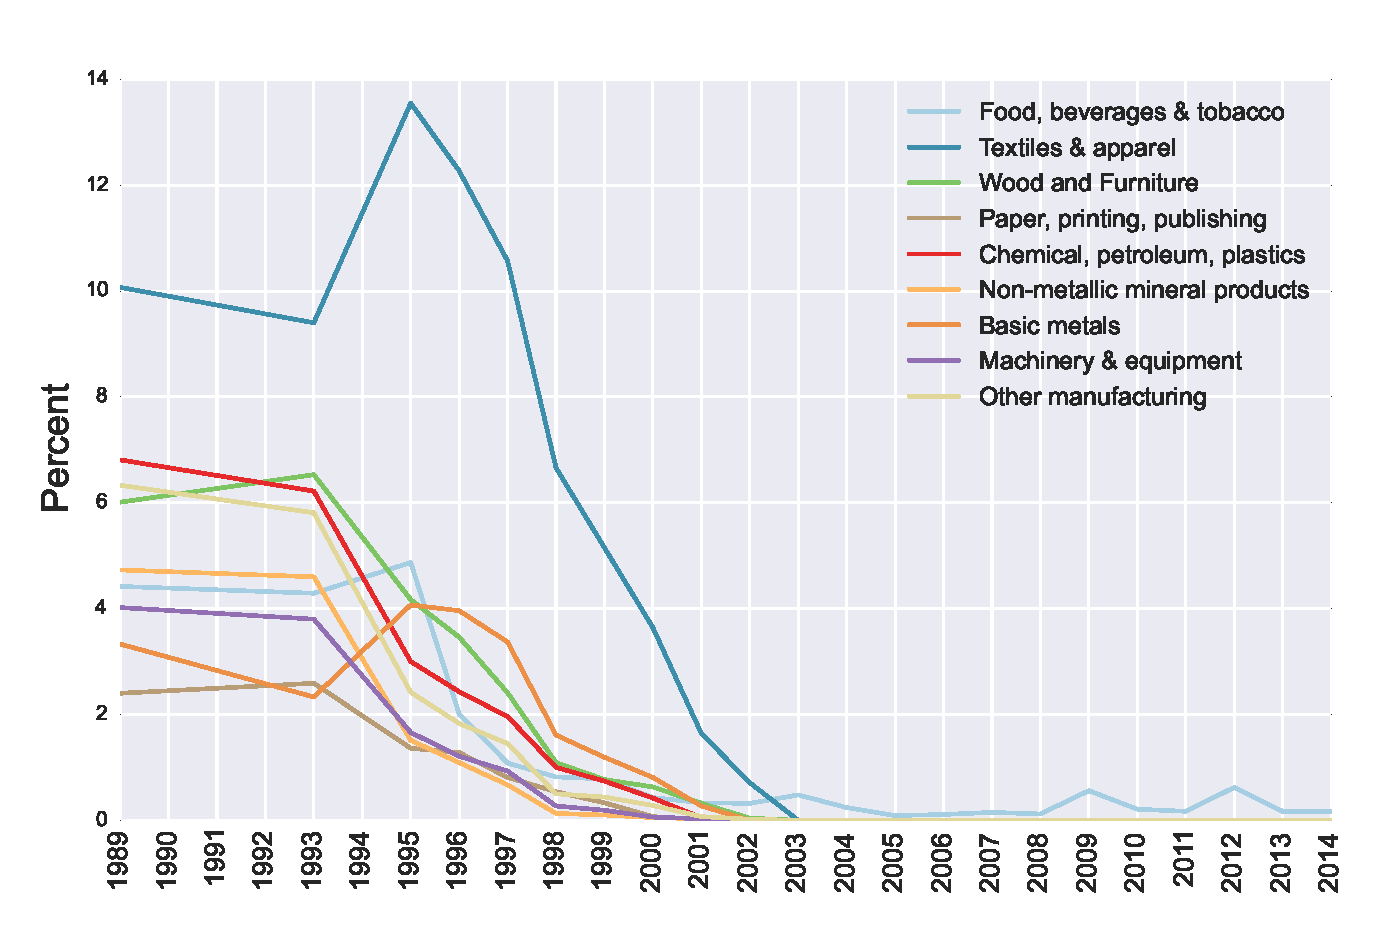
\includegraphics[scale=0.5]{tau_can_mex}
\label{fig:can_mex}
\end{figure} 

\begin{figure}[htpb]\centering
\caption{Canadian Tariff on U.S. Goods}\vspace{0.2cm}
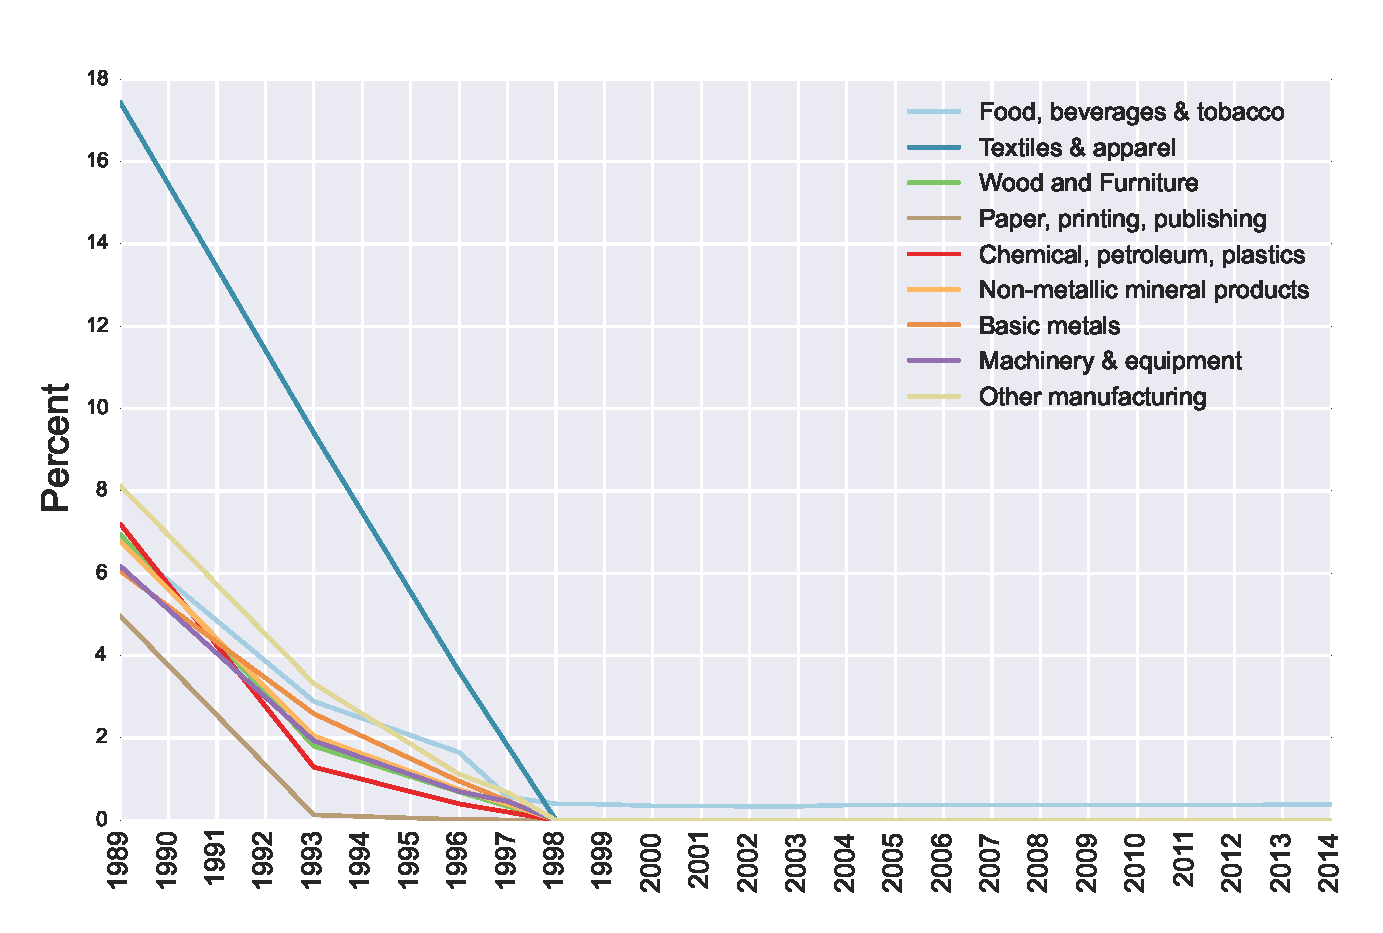
\includegraphics[scale=0.5]{tau_can_usa}
\label{fig:can_usa}
\end{figure}

\newpage

\begin{figure}[htpb]\centering
\caption{\small Mexican Tariff on Canadian Goods}\vspace{0.2cm}
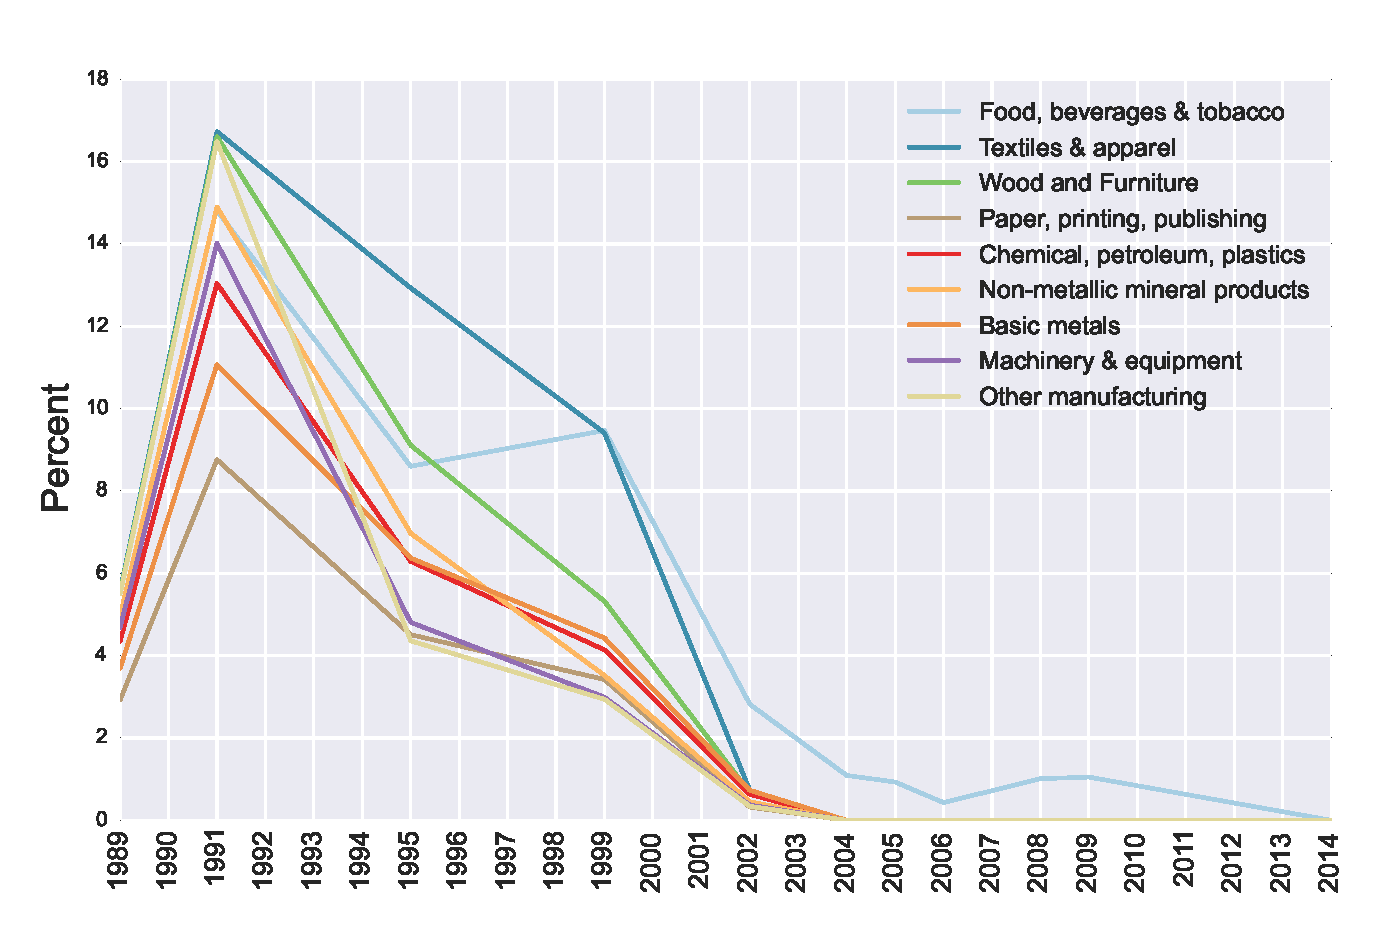
\includegraphics[scale=0.5]{tau_mex_can}
\label{fig:mex_can}
\end{figure}

\begin{figure}[htpb]\centering
\caption{\small Mexican Tariff on U.S. Goods}\vspace{0.2cm}
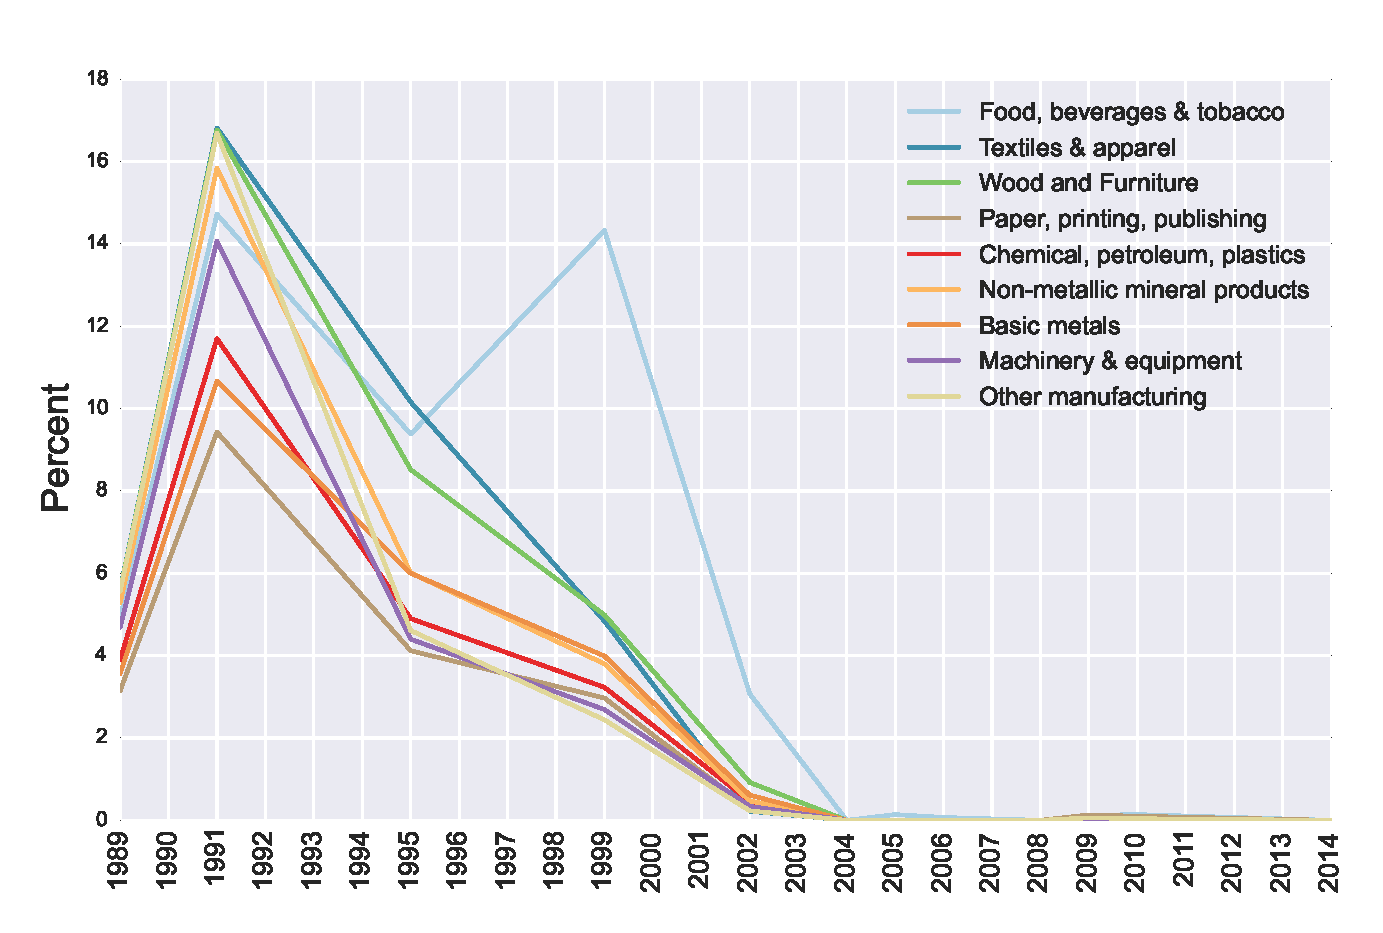
\includegraphics[scale=0.5]{tau_mex_usa}
\label{fig:mex_usa}
\end{figure}

\newpage

\begin{figure}[htpb]\centering
\caption{\small U.S. Tariff on Canadian Goods}\vspace{0.2cm}
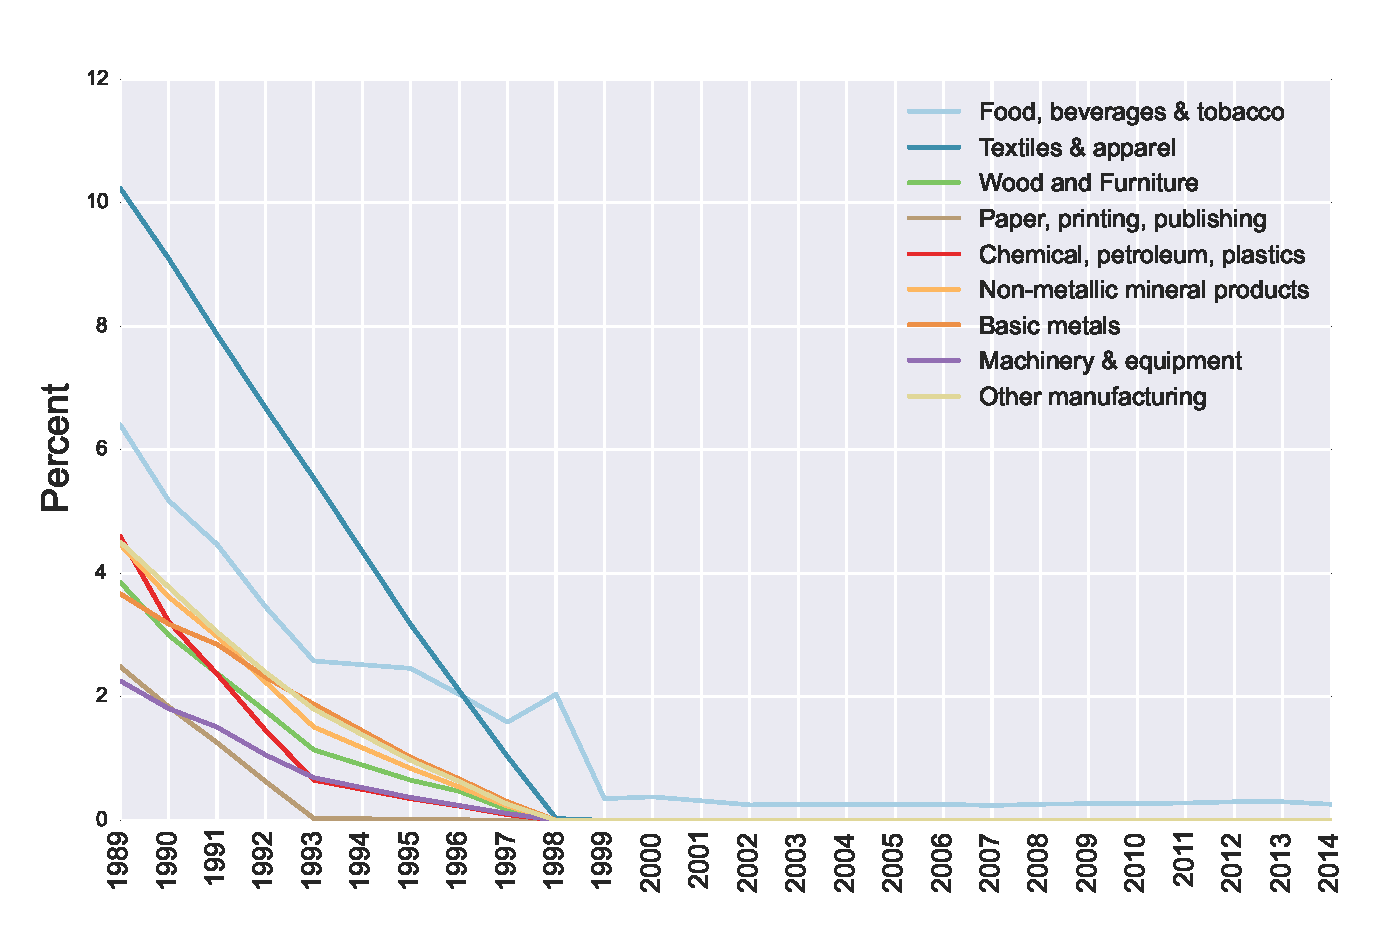
\includegraphics[scale=0.5]{tau_usa_can}
\label{fig:usa_can}
\end{figure}
 
\begin{figure}[htpb]\centering
\caption{\small U.S. Tariff on Mexican Goods}\vspace{0.2cm}
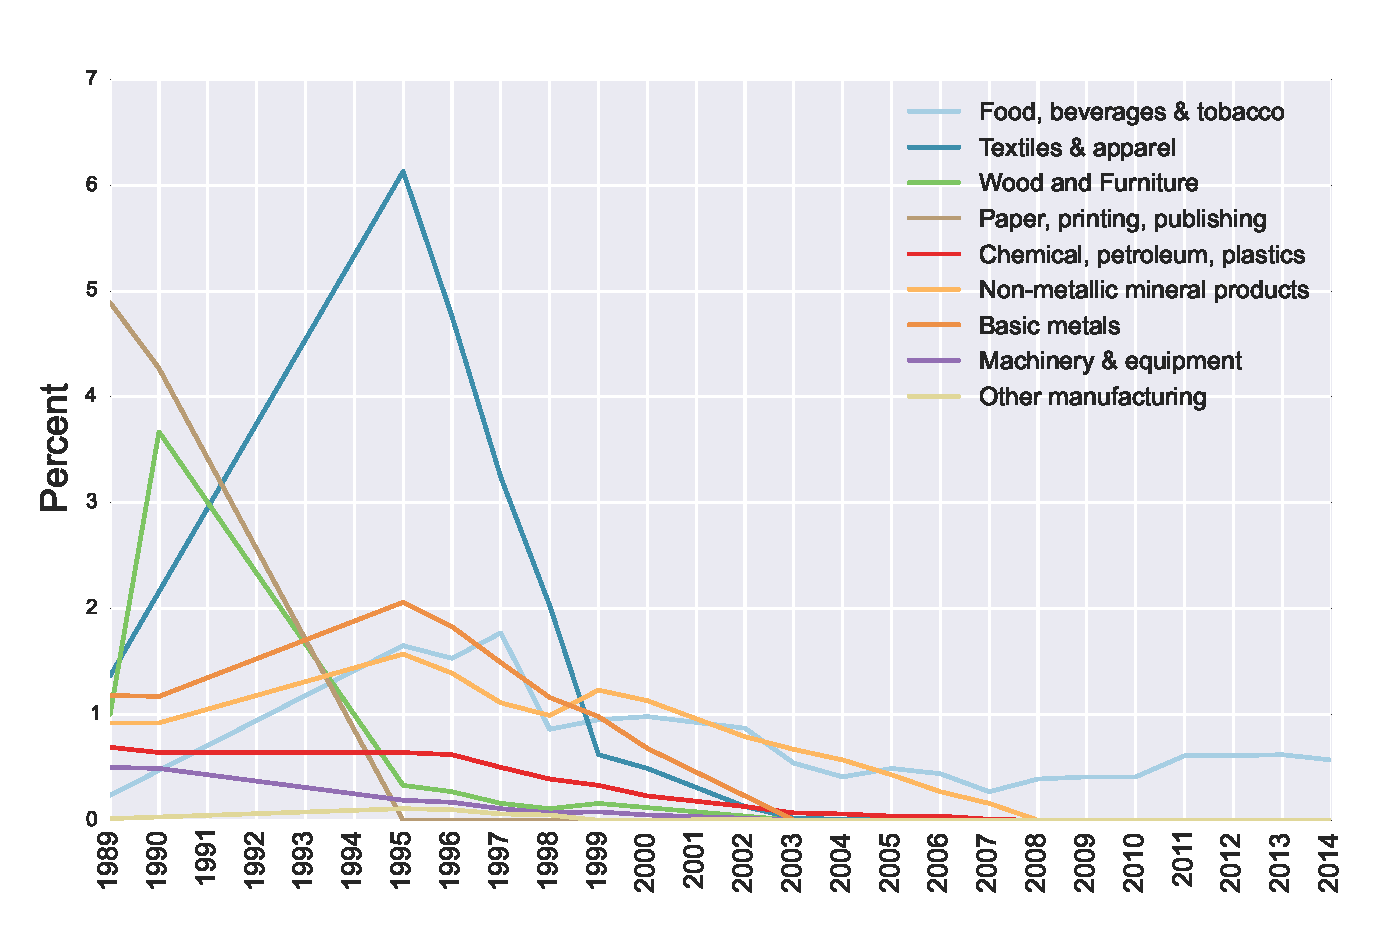
\includegraphics[scale=0.5]{tau_usa_mex}
\label{fig:usa_mex}
\end{figure}


\begin{center}
\begin{sidewaystable}

% Table created by stargazer v.5.0 by Marek Hlavac, Harvard University. E-mail: hlavac at fas.harvard.edu
% Date and time: Mon, Apr 28, 2014 - 18:37:50
% Requires LaTeX packages: rotating 
\begin{tabular}{@{\extracolsep{5pt}}lccccc} 
\\[-1.8ex]\hline 
\hline \\[-1.8ex] 
Statistic & \multicolumn{1}{c}{N} & \multicolumn{1}{c}{Mean} & \multicolumn{1}{c}{St. Dev.} & \multicolumn{1}{c}{Min} & \multicolumn{1}{c}{Max} \\ 
exp\_f & 702 & 76,233,571,691.000 & 198,643,966,085.000 & 399,038,863 & 1,890,000,000,000 \\ 
gdp\_can & 594 & 908.568 & 278.187 & 536.500 & 1,370.640 \\ 
gdp\_mex & 594 & 1,036.795 & 315.456 & 560.660 & 1,566.310 \\ 
gdp\_usa & 594 & 9,807.745 & 2,991.049 & 5,482.130 & 14,498.930 \\ 
cpi\_can & 675 & 79.697 & 12.487 & 56.340 & 100.000 \\ 
cpi\_mex & 675 & 48.219 & 32.559 & 1.560 & 100.000 \\ 
cpi\_usa & 675 & 75.546 & 14.894 & 50.300 & 100.000 \\ 
open\_ind\_can & 810 & 59.378 & 12.446 & 37.550 & 75.580 \\ 
open\_ind\_mex & 810 & 34.822 & 17.307 & 13.210 & 62.320 \\ 
open\_ind\_usa & 810 & 22.673 & 3.691 & 17.190 & 30.970 \\ 
ppi\_mex & 810 & 57.485 & 51.438 & 0.100 & 276.590 \\ 
tau\_s\_can\_mex & 540 & 1.829 & 3.193 & 0.000 & 17.780 \\ 
tau\_s\_can\_usa & 540 & 2.440 & 5.051 & 0.000 & 26.440 \\ 
tau\_s\_mex\_can & 405 & 8.654 & 8.751 & 0.000 & 30.530 \\ 
tau\_s\_mex\_usa & 405 & 7.611 & 8.552 & 0.000 & 28.800 \\ 
tau\_s\_usa\_can & 621 & 0.994 & 1.780 & 0.000 & 10.600 \\ 
tau\_s\_usa\_mex & 621 & 1.717 & 2.654 & 0.000 & 11.810 \\ 
\hline \\[-1.8ex] 
\end{tabular} 

\caption{Summary Statistics}
\label{tab:sumstats}
\end{sidewaystable}
\end{center}
\footnote{The majority of output tables in this paper has been produced using the stargazer package \citep{Hlavac2014}}

\newpage

\section{Appendix B: Conversion Table}

\begin{center}
\begin{table*}[ht] \caption{Manufacturing Sectors: ISIC Rev. 3 to ISIC Rev. 2 Conversion}\label{tb:isic_class}
{\small 
\hfill{}
\begin{tabular}{| p{8cm} | p{8cm} |} 
\hline
\textbf{ISIC Rev. 3}&\textbf{ISIC Rev. 2}\\
\hline
\hline
D15: Foods, products, and beverages &  31: Food, beverages, and tobacco\\
D16: Tobacco products & \\
\hline
D17: Textiles & \\
D18: Wearing apparel, dressing and dyeing of fur & 32: Textile, wearing apparel, and leather industries\\
D19: Tanning and dressing of leather, manufacture of luggage, handbags, saddlery, harness and footwear & \\
\hline
D20: Wood and of products of wood and cork, except furniture; manufacture of articles of straw and plaiting materials & 33:Wood and Wood Products, Including Furniture\\
\hline
D21: Paper and paper products & 34: Paper and paper products, printing and publishing\\ 
D22: Publishing, printing, and reproduction of recorded media & \\
\hline
D23: Coke, refined petroleum products and nuclear fuel & \\
D24: Chemicals and chemical products & 35: Chemical, petroleum, coal, rubber and plastic products\\
D25: Rubber and plastics products & \\
\hline
D26: Other non-metallic mineral products & 36: Non-metallic mineral products, except products of petroleum and coal\\
\hline
D27: Basic metals & 37: Basic Metal Industries\\
\hline
D28: Fabricated metal products, except machinery and equipment & \\
D29: Machinery and equipment n.e.c. & \\
D30: Office, accounting and computing machinery & \\
D31: Electrical machinery and apparatus n.e.c. & 38: Fabricated metal products, machinery and equipment\\
D32: Radio, television and communication equipment and apparatus & \\
D33: Medical, precision and optical instruments, watches and clocks & \\
D34: Motor vehicles, trailers and semi-trailers & \\
D35: Other transport equipment & \\
\hline
D36: Manufacture of furniture; manufacturing n.e.c. & 39: Other Manufacturing Industries\\
D37: Recycling & \\
\hline
\end{tabular}}
\end{table*}
\end{center}

\section{Appendix C: Regression Results}

\begin{table}
\tiny
\begin{center}\caption{Prices (Short Run), all country pairs\label{tb:prices_sr}}

% Table created by stargazer v.5.0 by Marek Hlavac, Harvard University. E-mail: hlavac at fas.harvard.edu
% Date and time: Mon, Apr 28, 2014 - 18:47:21
\begin{tabular}{@{\extracolsep{5pt}}lcc} 
\\[-1.8ex]\hline 
\hline \\[-1.8ex] 
 & \multicolumn{2}{c}{\textit{Dependent variable:}} \\ 
\cline{2-3} 
\\[-1.8ex] & \multicolumn{2}{c}{$\Delta \log \left(\frac{p}{p^*} \right)$} \\ 
\\[-1.8ex] & (1) & (2)\\ 
\hline \\[-1.8ex] 
 $\Delta \log \tau_t$ & 0.002 & 0.002 \\ 
  & (0.002) & (0.002) \\ 
  & & \\ 
 $\Delta \log \tau_t^*$ & $-$0.003$^{*}$ & $-$0.003 \\ 
  & (0.002) & (0.002) \\ 
  & & \\ 
 $\Delta \log \theta_t$ & $-$0.106$^{***}$ & $-$0.104$^{***}$ \\ 
  & (0.014) & (0.015) \\ 
  & & \\ 
 $\Delta \log \theta_t^*$ & 0.247$^{***}$ & 0.248$^{***}$ \\ 
  & (0.023) & (0.024) \\ 
  & & \\ 
 $\Delta \log D_t$ & 0.015 & 0.016 \\ 
  & (0.025) & (0.025) \\ 
  & & \\ 
 $\Delta \log D_t^*$ & $-$0.034 & $-$0.084 \\ 
  & (0.134) & (0.153) \\ 
  & & \\ 
\hline \\[-1.8ex] 
Observations & 320 & 320 \\ 
R$^{2}$ & 0.371 & 0.379 \\ 
\hline 
\hline \\[-1.8ex] 
\textit{Note:}  & \multicolumn{2}{r}{$^{*}$p$<$0.1; $^{**}$p$<$0.05; $^{***}$p$<$0.01} \\ 
 & \multicolumn{2}{r}{Fixed effects for country pair} \\ 
\end{tabular} 

\end{center}
\end{table}

\begin{table}
\tiny
\begin{center}\caption{Markups (Short Run), all country pairs\label{tb:markup_sr}}

% Table created by stargazer v.5.0 by Marek Hlavac, Harvard University. E-mail: hlavac at fas.harvard.edu
% Date and time: Thu, Apr 24, 2014 - 19:57:37
\begin{tabular}{@{\extracolsep{5pt}}lcccc} 
\\[-1.8ex]\hline 
\hline \\[-1.8ex] 
 & \multicolumn{4}{c}{\textit{Dependent variable:}} \\ 
\cline{2-5} 
\\[-1.8ex] & \multicolumn{4}{c}{$\Delta \log \left(\frac{\mu}{\mu^*} \right)$} \\ 
\\[-1.8ex] & (1) & (2) & (3) & (4)\\ 
\hline \\[-1.8ex] 
 $\Delta \log \tau_t$ & 0.001 & 0.001 & 0.001 & 0.001 \\ 
  & (0.001) & (0.001) & (0.001) & (0.001) \\ 
  & & & & \\ 
 $\Delta \log \tau_t^*$ & 0.00003 & 0.00003 & 0.0002 & 0.0002 \\ 
  & (0.001) & (0.001) & (0.001) & (0.001) \\ 
  & & & & \\ 
 $\Delta \log \theta$ &  &  & $-$0.024$^{***}$ & $-$0.024$^{***}$ \\ 
  &  &  & (0.005) & (0.006) \\ 
  & & & & \\ 
 $\Delta \log \theta^*$ &  &  & 0.028$^{***}$ & 0.028$^{***}$ \\ 
  &  &  & (0.009) & (0.009) \\ 
  & & & & \\ 
 $\Delta \log D_{t}$ & $-$0.003 & $-$0.002 & $-$0.005 & $-$0.003 \\ 
  & (0.009) & (0.009) & (0.009) & (0.009) \\ 
  & & & & \\ 
 $\Delta \log D_{t-1}$ & 0.049 & 0.006 & 0.037 & $-$0.008 \\ 
  & (0.050) & (0.056) & (0.049) & (0.055) \\ 
  & & & & \\ 
\hline \\[-1.8ex] 
Observations & 306 & 306 & 302 & 302 \\ 
R$^{2}$ & 0.009 & 0.006 & 0.109 & 0.107 \\ 
\hline 
\hline \\[-1.8ex] 
\textit{Note:}  & \multicolumn{4}{r}{$^{*}$p$<$0.1; $^{**}$p$<$0.05; $^{***}$p$<$0.01} \\ 
 & \multicolumn{4}{r}{Fixed effects for country pair} \\ 
\end{tabular} 

\end{center}
\end{table}

\begin{table}
\tiny
\begin{center} \caption{Productivity (Short Run), all country pairs\label{tb:productivity_sr}}

% Table created by stargazer v.5.1 by Marek Hlavac, Harvard University. E-mail: hlavac at fas.harvard.edu
% Date and time: Fri, Oct 02, 2015 - 13:51:58
\begin{tabular}{@{\extracolsep{5pt}}lcccccc} 
\\[-1.8ex]\hline 
\hline \\[-1.8ex] 
 & \multicolumn{6}{c}{\textit{Dependent variable:}} \\ 
\cline{2-7} 
\\[-1.8ex] & \multicolumn{6}{c}{$\Delta \log \left(\frac{z}{z^*} \right)$} \\ 
\\[-1.8ex] & (1) & (2) & (3) & (4) & (5) & (6)\\ 
\hline \\[-1.8ex] 
 $\Delta \log \tau_t$ & $-$0.009$^{***}$ & $-$0.009$^{***}$ & $-$0.018$^{***}$ & $-$0.002 & $-$0.018$^{***}$ & $-$0.002 \\ 
  & (0.003) & (0.003) & (0.005) & (0.006) & (0.005) & (0.006) \\ 
  & & & & & & \\ 
 $\Delta \log \tau_t^*$ & 0.006$^{*}$ & 0.006$^{*}$ & 0.010$^{**}$ & 0.011$^{*}$ & 0.010$^{**}$ & 0.011$^{*}$ \\ 
  & (0.003) & (0.003) & (0.004) & (0.006) & (0.004) & (0.006) \\ 
  & & & & & & \\ 
 $\Delta \log D_t$ & 0.146$^{***}$ & 0.145$^{***}$ & 0.200$^{***}$ & 0.056 & 0.201$^{***}$ & 0.051 \\ 
  & (0.056) & (0.054) & (0.072) & (0.118) & (0.070) & (0.114) \\ 
  & & & & & & \\ 
 $\Delta \log D_t^*$ & 0.015 & 0.035 & $-$0.097 & 0.541 & $-$0.095 & 0.716$^{*}$ \\ 
  & (0.089) & (0.083) & (0.091) & (0.484) & (0.088) & (0.399) \\ 
  & & & & & & \\ 
\hline \\[-1.8ex] 
Observations & 2,695 & 2,695 & 990 & 860 & 990 & 860 \\ 
R$^{2}$ & 0.007 & 0.006 & 0.022 & 0.006 & 0.021 & 0.008 \\ 
\hline 
\hline \\[-1.8ex] 
\textit{Note:}  & \multicolumn{6}{r}{$^{*}$p$<$0.1; $^{**}$p$<$0.05; $^{***}$p$<$0.01} \\ 
 & \multicolumn{6}{r}{(1),(3),(4): Fixed effects country-industry; (2),(5),(6): Fixed effect country pair} \\ 
\end{tabular} 

\end{center}
\end{table}

\begin{table}
\tiny
\begin{center}\caption{Prices (Long Run), all country pairs\label{tb:prices_lr}}

% Table created by stargazer v.5.1 by Marek Hlavac, Harvard University. E-mail: hlavac at fas.harvard.edu
% Date and time: Fri, Oct 02, 2015 - 13:14:33
\begin{tabular}{@{\extracolsep{5pt}}lcccccc} 
\\[-1.8ex]\hline 
\hline \\[-1.8ex] 
 & \multicolumn{6}{c}{\textit{Dependent variable:}} \\ 
\cline{2-7} 
\\[-1.8ex] & \multicolumn{6}{c}{$\Delta \log \left(\frac{p_t}{p_t^*} \right)$} \\ 
\\[-1.8ex] & (1) & (2) & (3) & (4) & (5) & (6)\\ 
\hline \\[-1.8ex] 
 $\Delta \log \tau_t$ & 0.001 & 0.001 & $-$0.001 & 0.005$^{**}$ & $-$0.001 & 0.004$^{**}$ \\ 
  & (0.001) & (0.001) & (0.002) & (0.002) & (0.002) & (0.002) \\ 
  & & & & & & \\ 
 $\Delta \log \tau_t^*$ & $-$0.001 & 0.00004 & $-$0.00004 & $-$0.002 & 0.0002 & 0.0004 \\ 
  & (0.001) & (0.001) & (0.002) & (0.002) & (0.002) & (0.002) \\ 
  & & & & & & \\ 
 $\Delta \log D_t$ & $-$0.031 & $-$0.025 & $-$0.063$^{**}$ & 0.008 & $-$0.061$^{**}$ & 0.023 \\ 
  & (0.023) & (0.021) & (0.031) & (0.041) & (0.030) & (0.040) \\ 
  & & & & & & \\ 
 $\Delta \log D_t^*$ & 0.038 & 0.028 & 0.038 & 0.366$^{**}$ & 0.036 & 0.132 \\ 
  & (0.036) & (0.033) & (0.039) & (0.174) & (0.037) & (0.141) \\ 
  & & & & & & \\ 
 $\log \left(\frac{p_{t-1}}{p_{t-1}^*} \right)$ & $-$0.123$^{***}$ & $-$0.118$^{***}$ & $-$0.121$^{***}$ & $-$0.149$^{***}$ & $-$0.118$^{***}$ & $-$0.137$^{***}$ \\ 
  & (0.006) & (0.005) & (0.010) & (0.010) & (0.009) & (0.009) \\ 
  & & & & & & \\ 
 $\log \tau_{t-1}$ & $-$0.001 & $-$0.001 & $-$0.001 & $-$0.0003 & $-$0.001 & $-$0.001 \\ 
  & (0.001) & (0.001) & (0.002) & (0.002) & (0.002) & (0.002) \\ 
  & & & & & & \\ 
 $\log \tau_{t-1}^*$ & $-$0.002 & $-$0.00002 & $-$0.0003 & $-$0.006$^{***}$ & 0.0004 & $-$0.002 \\ 
  & (0.001) & (0.001) & (0.002) & (0.002) & (0.002) & (0.001) \\ 
  & & & & & & \\ 
 $\log L_{t-1}$ & $-$0.570$^{***}$ & $-$0.541$^{***}$ & $-$0.497$^{***}$ & $-$0.775$^{***}$ & $-$0.480$^{***}$ & $-$0.734$^{***}$ \\ 
  & (0.082) & (0.077) & (0.136) & (0.139) & (0.131) & (0.135) \\ 
  & & & & & & \\ 
 $\log L_{t-1}^*$ & 0.466$^{***}$ & 0.458$^{***}$ & 0.400$^{***}$ & 0.611$^{***}$ & 0.396$^{***}$ & 0.616$^{***}$ \\ 
  & (0.080) & (0.076) & (0.132) & (0.138) & (0.126) & (0.133) \\ 
  & & & & & & \\ 
\hline \\[-1.8ex] 
Observations & 2,769 & 2,769 & 1,021 & 881 & 1,021 & 881 \\ 
R$^{2}$ & 0.184 & 0.181 & 0.192 & 0.246 & 0.187 & 0.224 \\ 
\hline 
\hline \\[-1.8ex] 
\textit{Note:}  & \multicolumn{6}{r}{$^{*}$p$<$0.1; $^{**}$p$<$0.05; $^{***}$p$<$0.01} \\ 
 & \multicolumn{6}{r}{Fixed effects for country pair} \\ 
\end{tabular} 

\end{center}
\end{table}


\begin{table}
\tiny
\begin{center}\caption{Markups (Long Run), all country pairs\label{tb:markup_lr}}

% Table created by stargazer v.5.0 by Marek Hlavac, Harvard University. E-mail: hlavac at fas.harvard.edu
% Date and time: Thu, Apr 24, 2014 - 19:57:52
\begin{tabular}{@{\extracolsep{5pt}}lcccc} 
\\[-1.8ex]\hline 
\hline \\[-1.8ex] 
 & \multicolumn{4}{c}{\textit{Dependent variable:}} \\ 
\cline{2-5} 
\\[-1.8ex] & \multicolumn{4}{c}{$\Delta \log \left(\frac{\mu}{\mu^*} \right)$} \\ 
\\[-1.8ex] & (1) & (2) & (3) & (4)\\ 
\hline \\[-1.8ex] 
 $\Delta \log \tau$ & 0.001 & 0.0004 & 0.001 & 0.0005 \\ 
  & (0.001) & (0.001) & (0.001) & (0.001) \\ 
  & & & & \\ 
 $\Delta \log \tau^*$ & 0.001 & 0.001 & 0.00002 & 0.0003 \\ 
  & (0.001) & (0.001) & (0.001) & (0.001) \\ 
  & & & & \\ 
 $\Delta \log \theta$ &  &  & $-$0.032$^{***}$ & $-$0.027$^{***}$ \\ 
  &  &  & (0.006) & (0.006) \\ 
  & & & & \\ 
 $\Delta \log \theta^*$ &  &  & 0.048$^{***}$ & 0.095$^{***}$ \\ 
  &  &  & (0.010) & (0.016) \\ 
  & & & & \\ 
 $\Delta \log D_t$ & $-$0.0004 & 0.012 & $-$0.004 & 0.006 \\ 
  & (0.009) & (0.008) & (0.009) & (0.007) \\ 
  & & & & \\ 
 $\Delta \log D_t^*$ & 0.027 & $-$0.055 & 0.034 & $-$0.063 \\ 
  & (0.053) & (0.050) & (0.051) & (0.047) \\ 
  & & & & \\ 
 $\log \left(\frac{\mu_{t-1}}{\mu_{t-1}^*} \right)$ & 0.010 & $-$0.460$^{***}$ & 0.003 & $-$0.454$^{***}$ \\ 
  & (0.007) & (0.042) & (0.007) & (0.039) \\ 
  & & & & \\ 
 $\tau_{t-1}$ & $-$0.001 & $-$0.002$^{**}$ & $-$0.001 & $-$0.002$^{**}$ \\ 
  & (0.001) & (0.001) & (0.001) & (0.001) \\ 
  & & & & \\ 
 $\tau_{t-1}^*$ & 0.001 & 0.001$^{*}$ & $-$0.0001 & 0.001 \\ 
  & (0.001) & (0.001) & (0.001) & (0.001) \\ 
  & & & & \\ 
 $\log \theta_{t-1}$ &  &  & $-$0.010$^{***}$ & $-$0.010$^{*}$ \\ 
  &  &  & (0.003) & (0.005) \\ 
  & & & & \\ 
 $\log \theta_{t-1}^*$ &  &  & 0.008$^{**}$ & 0.037$^{***}$ \\ 
  &  &  & (0.003) & (0.010) \\ 
  & & & & \\ 
 $L_{t-1}$ & $-$0.156$^{*}$ & $-$0.128$^{*}$ & $-$0.255$^{***}$ & $-$0.185$^{***}$ \\ 
  & (0.080) & (0.068) & (0.080) & (0.066) \\ 
  & & & & \\ 
 $L_{t-1}^*$ & 0.139$^{*}$ & 0.104 & 0.230$^{***}$ & 0.138$^{**}$ \\ 
  & (0.081) & (0.068) & (0.081) & (0.068) \\ 
  & & & & \\ 
\hline \\[-1.8ex] 
Observations & 306 & 306 & 302 & 302 \\ 
R$^{2}$ & 0.040 & 0.332 & 0.183 & 0.491 \\ 
\hline 
\hline \\[-1.8ex] 
\textit{Note:}  & \multicolumn{4}{r}{$^{*}$p$<$0.1; $^{**}$p$<$0.05; $^{***}$p$<$0.01} \\ 
 & \multicolumn{4}{r}{Fixed effects for country pair} \\ 
\end{tabular} 

\end{center}
\end{table}

\begin{table}
\tiny
\begin{center}\caption{Productivity (Long Run), all country pairs\label{tb:productivity_lr}}

% Table created by stargazer v.5.0 by Marek Hlavac, Harvard University. E-mail: hlavac at fas.harvard.edu
% Date and time: Thu, Apr 24, 2014 - 19:57:58
\begin{tabular}{@{\extracolsep{5pt}}lcccc} 
\\[-1.8ex]\hline 
\hline \\[-1.8ex] 
 & \multicolumn{4}{c}{\textit{Dependent variable:}} \\ 
\cline{2-5} 
\\[-1.8ex] & \multicolumn{4}{c}{$\Delta \log \left(\frac{z}{z^*} \right)$} \\ 
\\[-1.8ex] & (1) & (2) & (3) & (4)\\ 
\hline \\[-1.8ex] 
 $\Delta \log \tau_t$ & 0.0002 & $-$0.001 & 0.004 & 0.003 \\ 
  & (0.005) & (0.004) & (0.004) & (0.004) \\ 
  & & & & \\ 
 $\Delta \log \tau_t^*$ & 0.001 & 0.004 & $-$0.001 & 0.002 \\ 
  & (0.005) & (0.005) & (0.005) & (0.005) \\ 
  & & & & \\ 
 $\Delta \log \theta$ &  &  & $-$0.245$^{***}$ & $-$0.214$^{***}$ \\ 
  &  &  & (0.040) & (0.042) \\ 
  & & & & \\ 
 $\Delta \log \theta^*$ &  &  & 0.574$^{***}$ & 0.451$^{***}$ \\ 
  &  &  & (0.070) & (0.131) \\ 
  & & & & \\ 
 $\Delta \log D_t$ & $-$0.428$^{*}$ & 0.409$^{*}$ & $-$0.179 & 0.262 \\ 
  & (0.246) & (0.221) & (0.210) & (0.208) \\ 
  & & & & \\ 
 $\Delta \log D_t^*$ & 0.336 & $-$0.427 & 0.167 & $-$0.175 \\ 
  & (0.393) & (0.358) & (0.345) & (0.353) \\ 
  & & & & \\ 
 $\log \left(\frac{z_{t-1}}{z_{t-1}^*} \right)$ & $-$0.145$^{***}$ & $-$0.348$^{***}$ & $-$0.089$^{***}$ & $-$0.308$^{***}$ \\ 
  & (0.016) & (0.022) & (0.015) & (0.033) \\ 
  & & & & \\ 
 $\log \tau_{t-1}$ & $-$0.008 & $-$0.009$^{*}$ & $-$0.007 & $-$0.006 \\ 
  & (0.006) & (0.005) & (0.005) & (0.005) \\ 
  & & & & \\ 
 $\log \tau_{t-1}^*$ & 0.006 & 0.013$^{**}$ & 0.0004 & 0.006 \\ 
  & (0.005) & (0.005) & (0.005) & (0.005) \\ 
  & & & & \\ 
 $\log \theta_{t-1}$ &  &  & $-$0.012 & $-$0.092$^{**}$ \\ 
  &  &  & (0.021) & (0.043) \\ 
  & & & & \\ 
 $\log \theta_{t-1}^*$ &  &  & $-$0.010 & 0.119 \\ 
  &  &  & (0.021) & (0.078) \\ 
  & & & & \\ 
 $\log L_{t-1}$ & 0.569 & $-$1.531$^{***}$ & $-$0.523 & $-$1.625$^{***}$ \\ 
  & (0.623) & (0.559) & (0.539) & (0.538) \\ 
  & & & & \\ 
 $\log L_{t-1}^*$ & $-$0.777 & 1.740$^{***}$ & 0.198 & 1.416$^{***}$ \\ 
  & (0.636) & (0.568) & (0.547) & (0.543) \\ 
  & & & & \\ 
 $\log w_{t-1}$ & 0.160$^{**}$ & 0.181$^{**}$ & 0.068 & 0.216$^{**}$ \\ 
  & (0.063) & (0.090) & (0.058) & (0.100) \\ 
  & & & & \\ 
 $\log w_{t-1}^*$ & $-$0.230$^{***}$ & $-$0.584$^{***}$ & $-$0.063 & $-$0.129 \\ 
  & (0.069) & (0.117) & (0.062) & (0.142) \\ 
  & & & & \\ 
\hline \\[-1.8ex] 
Observations & 324 & 324 & 320 & 320 \\ 
R$^{2}$ & 0.290 & 0.543 & 0.510 & 0.613 \\ 
\hline 
\hline \\[-1.8ex] 
\textit{Note:}  & \multicolumn{4}{r}{$^{*}$p$<$0.1; $^{**}$p$<$0.05; $^{***}$p$<$0.01} \\ 
 & \multicolumn{4}{r}{Fixed effects for country pair or industry/country pair} \\ 
\end{tabular} 

\end{center}
\end{table} 

\chapter{Conclusion} %preface is not numbered
\markboth{\MakeUppercase{\thechapter. CONCLUSION }}{CONCLUSION}
Throughout this thesis, an outline of affine term structure models is provided. This particular class of term structure models has been made very popular in recent years due to its ability to capture the dynamics of yields both across their time series and cross-section and its ease in imposing the absence of arbitrage, allowing in turn the obtention of adaptable risk premia specifications. Affine term structure models have the advantage of allowing various extensions, in a wide range, to their basic primary setup, asserting their importance in the literature. However, difficulties do arise in their estimation and in the interpretation of the latent factors used. This thesis addresses both problems by utilizing a specific structure to the factor loadings, known as the Nelson-Siegel method. The estimation of this term structure model not only circumvents the global optimum issues but further provides some interpretation to the factors, given the level, slope and curvature factors of the Nelson-Siegel interpolation are not only intuitive in their nature, but also have reliable macroeconomic links.  % level with inflation and slope with economic activity

The present thesis introduces and employs dynamic term structure models to macroeconomic and financial research questions. More precisely, this study initially pertains to financial markets by establishing a tie between interest rates and exchange rates. The study follows by concerning itself with macroeconomic objectives, by exploiting the relationship between yields and inflation.

In a first instance, this study exploits a theoretical relationship between interest rates and exchange rates, namely the uncovered interest rate parity, with the aim to extract currency risk premia through a bilateral affine term structure model with stochastic volatility. The method proposed consists of developing an affine Arbitrage-Free class of dynamic Nelson-Siegel term structure models (AFNS) with stochastic volatility to obtain the domestic and foreign discount rate variations, which in turn are used to derive a representation of exchange rate depreciations. The manipulation of no-arbitrage restrictions allows to endogenously capture currency risk premia. The estimation exercise comprises of a state-space analysis using the Kalman filter. The imposition of the Dynamic Nelson-Siegel (DNS) structure allows for a tractable and robust estimation, offering significant computational benefits, whilst no-arbitrage restrictions enforce the model with theoretically appealing properties. Empirical findings suggest that estimated currency risk premia are able to account for the forward premium puzzle. 

In a second instance, inflation expectations and inflation risk premia are derived using a shadow rate class of term structure models. In response to the recent financial crisis, the Bank of England reduced short term interest rates to 0.5\%. With such low short term rates, traditional term structure models are likely to be inappropriate for estimating inflation expectations and risk premia, because expectations based on such models might implicitly violate the zero lower bound condition. In this segment both the nominal and real UK term structure of interest rates are studied, using the dynamic term structure model introduced by \cite{christensen_2013}, which imposes the non-negativity of nominal short maturity rates. Estimates of the term premia, inflation risk premia and market-implied inflation expectations are provided. Findings indicate that the zero lower bound specification is necessary to reflect countercyclicality in nominal term premia projections and that medium and long term inflation expectations have been contained within narrower bounds since the early 1990s, suggesting monetary policy credibility after the introduction of inflation targeting.

For my future research projects, I wish to draw from the analysis and discussion of this thesis and elaborate further on this strand of the literature, this time emphasizing on the joint effect of monetary economics and finance on asset prices, financial markets and monetary policy. Two main perspectives emerge within my research agenda. A potential project, that inclines more towards macroeconomic concepts, consists in building an extension of the two above-mentioned models by constructing a Taylor rule type of model which would further extend to include growth. Furthermore, an alternative suggests to further exploit the interaction between macroeconomic and financial data to explore a gap in the literature. Specifically, the study includes providing an economic interpretation to the latent factors, used in the state-space representation, by venturing towards macro-finance models and high frequency data. This analysis is built on the prior belief that assets are affected by macroeconomic conditions but simultaneously suffer from microstructure phenomena. %This analysis has the potential of being conducted in a Bayesian setting, due to the large dimensionality of the data. 

Notwithstanding the extensions listed above, it is crucial to note that the most important message to draw from this thesis is that the literature on risk premia is still at its infancy due to the striking complexity involved in estimating an unobservable variable which nonetheless contains a very rich informational content. In turn, in future research, I wish to investigate the sensitivity of the price of risk, and consequently of risk premia, to different specifications in the mean reversion matrix of the states' dynamics. The aim is to determine a preferred specification for dynamic term structure models using a Bayesian shrinkage estimation approach.

To conclude, this thesis builds a spherical account of the versatility of affine models by implementing them to distinct monetary finance applications. Several of the pending issues in the literature are addressed and the grounds for future interesting questions are paved. 
%In my fourth paper, the UK yield curve is modeled and forecasted in a data-rich environment, which includes the entire yield curve as well as macroeconomic variables. The estimation uses a Bayesian vector autoregression, whilst different priors and tightness levels are examined.
 
%Further, I elaborate on the incapacity of term structure models, so far, to capture the two first moments simultaneously. To this end, I consider using unspanned stochastic volatility to jointly capture the cross-section of conditional yields and the volatility of yields.

%I also consider including unspanned stochastic volatility to jointly capture the cross-section of conditional yields and their volatility.


\begin{spacing}{1.5}
\bibliographystyle{aer}
\bibliography{thesis_bibliography}
\newpage
\end{spacing}

\end{document}
